
\chapter{Complex Variables}
\section*{Introduction}
Our journey through calculus has taken us from single-variable functions to multivariable calculus in $\mathbb{R}^2$ and $\mathbb{R}^3$. Now, we turn to complex variables—not an esoteric detour but a natural extension of multidimensional calculus. The complex plane provides a fresh perspective on two-dimensional space, reshaping our understanding of functions, derivatives, and integrals.\\

\noindent The complex plane is isomorphic to $\mathbb{R}^2$ -- a fancy way of saying there is a one-to-one correspondence preserving mathematical operations. Writing $z = x + iy$ simply recasts $(x,y)$ in a new framework. Yet, with complex multiplication and division, stunning geometric patterns emerge—multiplying by $i$ corresponds to a 90-degree rotation, blending algebra and geometry in ways real analysis only hints at.\\

\noindent Concepts from vector calculus, such as line integrals and Green’s theorem, reappear in unexpected ways. Complex line integrals, though syntactically similar to real ones, exhibit striking properties—paths can often be deformed without altering the integral, mirroring conservative vector fields. The complex derivative, when it exists, ensures not just differentiability but analyticity, a property far stronger than in real analysis.\\

\noindent This journey promises both challenges and insights. Though the ideas may seem abstract at first, they build naturally on your knowledge, unifying and transforming familiar calculus concepts. Complex analysis reveals profound symmetries and patterns, making it a cornerstone of modern mathematics.



\newpage 



\lecture{The Complex Number System} \index{Complex Numbers}

\noindent Our journey through multivariable calculus has equipped us with tools to analyze functions of multiple real variables. However, there exists another number system—one that extends our familiar real numbers in profound and beautiful ways. This system of complex numbers not only helps us solve seemingly impossible equations but also provides deep insights into geometry, physics, and the very nature of mathematical structure itself.

\subsection*{Historical Development and Motivation}

\noindent The story of complex numbers begins with a mathematical impossibility—or what seemed impossible at the time. Consider the equation:
\[
x^2 + 1 = 0
\]

\noindent In the real number system, this equation has no solution. After all, any real number squared must be non-negative, so adding 1 can never yield zero. Yet mathematicians of the 16th century, particularly in their work on cubic equations, found themselves forced to work with expressions involving square roots of negative numbers. \\
%https://commons.wikimedia.org/wiki/File:Girolamo_Cardano._Stipple_engraving_by_R._Cooper._Wellcome_V0001004.jpg
\begin{figure}[H]
\centering
\includegraphics[width=0.3\textwidth]{chapters/chp7_pics/girolamo.jpg}
\caption{\textit{Girolamo Cardano, engraving by R. Cooper Wellcome}}
\label{girolamo}
\end{figure}

\noindent The Italian mathematician Girolamo Cardano, in his 1545 work \textit{Ars Magna}, presented a method for solving cubic equations that inevitably led to these ``impossible" quantities. Even more remarkably, by manipulating these supposedly impossible numbers according to normal algebraic rules, he obtained correct real number solutions. This suggested something profound: these ``imaginary" quantities, while seemingly nonsensical, somehow encoded real mathematical truth. \\

\noindent The modern understanding of complex numbers emerged gradually through the work of mathematicians like Euler, Gauss, and Cauchy, who showed that far from being mere computational tools, complex numbers form a coherent and beautiful mathematical system with deep connections to geometry, analysis, and physics. The term ``imaginary" is somewhat misleading, as complex analysis has tangible physical applications. In my view, it was a missed opportunity not to adopt Gauss's term ``lateral numbers" instead, which more aptly reflects their geometric nature and maintains their tangibility.

\subsection*{Algebraic Form and Fundamental Properties} \index{Properties of Complex Numbers}

\noindent Let's begin our formal development. We define the \textbf{imaginary unit} $i$ as a quantity satisfying:
\[
i^2 = -1
\]

\noindent This single definition opens up an entirely new number system. A \textbf{complex number} is an expression of the form:
\[
z = a + bi
\]
where $a$ and $b$ are real numbers. We call $a$ the \textbf{real part} and $b$ the \textbf{imaginary part} of $z$, denoted:
\[
\Re(z) = a \quad \text{and} \quad \Im(z) = b
\]

\noindent Sometimes you might see $\mathfrak{R}(z)$ and $\mathfrak{I}(z)$ in other texts to represent real and imaginary parts respectively. The set of all complex numbers, denoted $\mathbb{C}$, forms a field—it satisfies all the familiar properties of arithmetic (commutativity, associativity, distributivity, etc.) and every non-zero complex number has a multiplicative inverse. This makes $\mathbb{C}$ a natural extension of $\mathbb{R}$, the real numbers. However, you may notice that one fundamental arithmetic property is absent: order. Unlike real numbers, complex numbers cannot be meaningfully compared using inequalities, as there is no natural way to define \( a < b \) when \( a, b \in \mathbb{C} \). We will explore this limitation in more detail later. \\


\noindent Indeed, we can view $\mathbb{R}$ as a subset of $\mathbb{C}$ by identifying each real number $r$ with the complex number $r + 0i$. This embedding preserves all algebraic operations, meaning complex arithmetic agrees with real arithmetic when applied to real numbers.

\subsection*{The Complex Plane and Geometric Interpretation} \index{Argand Plane}

\noindent One of the most powerful aspects of complex numbers is their geometric interpretation. Just as real numbers correspond to points on a line, complex numbers naturally correspond to points in a plane. This \textbf{complex plane} (also called the \textbf{Argand plane} after Jean-Robert Argand) represents the complex number $a + bi$ as the point with coordinates $(a,b)$. \\

\noindent This geometric view transforms algebraic operations into geometric ones:
\begin{itemize}
    \item Addition of complex numbers corresponds to vector addition in the plane
    \item Multiplication by a real number corresponds to scaling
    \item Multiplication by $i$ corresponds to a 90-degree counterclockwise rotation
\end{itemize}

\noindent To see why multiplication by $i$ represents rotation, consider its effect:
\[
i(a + bi) = ai + bi^2 = ai + b(-1) = -b + ai
\]

\noindent This transforms the point $(a,b)$ to the point $(-b,a)$, which is exactly what a 90-degree counterclockwise rotation does! \\

\begin{figure}[H]
\centering
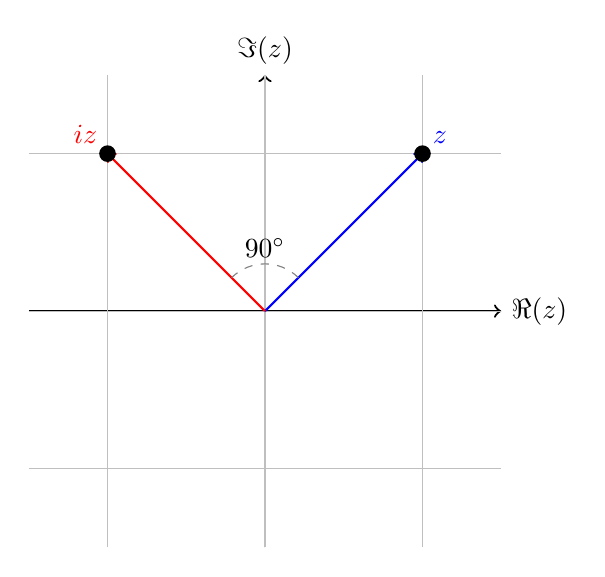
\begin{tikzpicture}[scale=2]
  % Draw axes with thicker lines
  \draw[->, thick] (-1.5,0) -- (1.5,0) node[right] {$\Re(z)$};
  \draw[->, thick] (0,-1.5) -- (0,1.5) node[above] {$\Im(z)$};

  % Draw grid lines
  \draw[lightgray,thin] (-1.5,-1.5) grid (1.5,1.5);

  % Define points
  \coordinate (P) at (1,1);
  \coordinate (Q) at (-1,1);

  % Draw original vector and its rotation
  \draw[blue,thick,->] (0,0) -- (P) node[above right] {$z$};
  \draw[red,thick,->] (0,0) -- (Q) node[above left] {$iz$};

  % Draw rotation arc from 45° to 135° (i.e., a 90° rotation)
  \draw[gray,dashed] ({0.3*cos(45)},{0.3*sin(45)}) arc (45:135:0.3);
  \node at (0,0.4) {$90^\circ$};

  % Mark points
  \fill (P) circle (1.5pt);
  \fill (Q) circle (1.5pt);

\end{tikzpicture}
\caption{\textit{Multiplication by $i$ rotates a complex number $90^\circ$ counterclockwise about the origin on the Argand plane.}}
\label{fig:complex-rotation}
\end{figure}


\subsection*{Basic Operations and Their Geometric Meaning}

\noindent Let's examine how the basic operations on complex numbers manifest geometrically. For two complex numbers $z_1 = a + bi$ and $z_2 = c + di$:

\begin{enumerate}
    \item \textbf{Addition:} 
    \[
    z_1 + z_2 = (a + c) + (b + d)i
    \]
    This corresponds to vector addition in the plane, following the parallelogram law.
    
    \item \textbf{Subtraction:}
    \[
    z_1 - z_2 = (a - c) + (b - d)i
    \]
    This corresponds to vector subtraction.
    
    \item \textbf{Multiplication:}
    \[
    z_1z_2 = (ac - bd) + (ad + bc)i
    \]
    This formula, while algebraically straightforward, hides a beautiful geometric interpretation we'll uncover when we study polar form.
\end{enumerate}

\subsection*{Complex Conjugates and Absolute Values} \index{Complex Conjugate} \index{Modulus}
\noindent For any complex number $z = a + bi$, its \textbf{complex conjugate}, denoted $\overline{z}$ or $z^*$, is defined as:
\[
\overline{z} = a - bi
\]
\noindent Geometrically, the conjugate reflects $z$ across the real axis. This operation has several crucial properties:
\begin{itemize}
\item $\overline{(\overline{z})} = z$
\item $\overline{z_1 + z_2} = \overline{z_1} + \overline{z_2}$
\item $\overline{z_1z_2} = \overline{z_1}\cdot\overline{z_2}$
\item $z\cdot\overline{z} = a^2 + b^2$ (always a non-negative real number)
\end{itemize}
\noindent The last property leads us to define the \textbf{absolute value} or \textbf{modulus} of a complex number:
\[
|z| = \sqrt{z\cdot\overline{z}} = \sqrt{a^2 + b^2}
\]
\noindent This definition generalizes the absolute value of real numbers and has a clear geometric interpretation: $|z|$ is the distance from $z$ to the origin in the complex plane. Now because the complex plane loses the property of number ordering, the modulus will be our primary tool in order to express distance and inequality between values and functions. \\

\noindent A fundamental concept in complex analysis is that an equation of the form $|z - z_0| = r$ describes a circle in the complex plane centered at $z_0$ with radius $r$. To understand why, let $z = x + yi$ and $z_0 = a + bi$. Then:
\begin{align*}
|z - z_0| &= r \
|(x + yi) - (a + bi)| &= r \
|(x-a) + (y-b)i| &= r \
\sqrt{(x-a)^2 + (y-b)^2} &= r
\end{align*}
\noindent This geometric interpretation makes the modulus an essential tool for describing regions in the complex plane. For instance, $|z| < r$ describes the interior of a circle centered at the origin with radius $r$, while $|z-z_1| < |z-z_2|$ describes all points closer to $z_1$ than to $z_2$.


\begin{figure}[H]
\centering
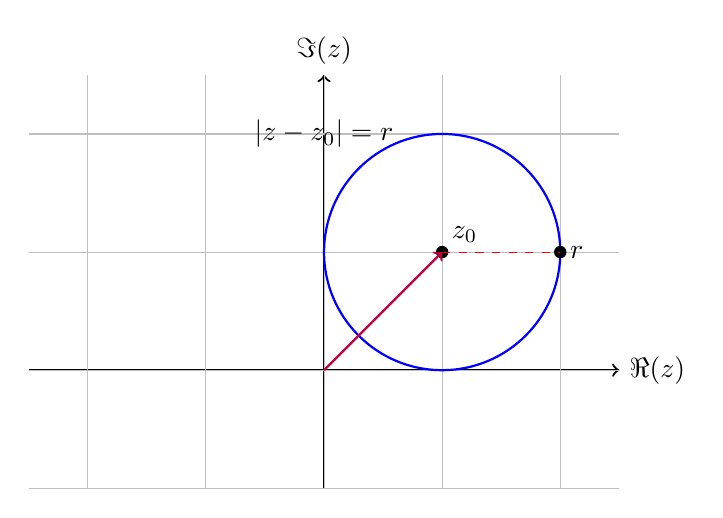
\begin{tikzpicture}[scale=1.5]
% Draw axes with thicker lines
\draw[->, thick] (-2.5,0) -- (2.5,0) node[right] {$\Re(z)$};
\draw[->, thick] (0,-1) -- (0,2.5) node[above] {$\Im(z)$};

% Extend grid beyond the circle for better spacing
\draw[lightgray,thin] (-2.5,-1) grid (2.5,2.5);

% Draw the circle |z - (1+i)| = 1 with more spacing
\draw[blue, thick] (1,1) circle (1);

% Draw center point
\fill (1,1) circle (1.5pt) node[above right] {$z_0$};

% Draw a point on the circle
\fill (2,1) circle (1.5pt) node[right] {$r$};

% Draw radius
\draw[red, dashed] (1,1) -- (2,1) node[midway,above] {};

% Draw arrow from origin to center of the circle
\draw[->, thick, purple] (0,0) -- (1,1) node[midway,below left] { };

% Label the circle
\node at (0,2) {$|z-z_0| = r$};
\end{tikzpicture}
\caption{\textit{The equation $|z-z_0| = r$ describes all points $z$ that are exactly distance $r$ from the point $z_0$, forming a circle.}}
\label{fig:modulus-circle}
\end{figure}

\exampleline
\begin{example}
Express the complex fraction $\frac{2-3i}{4+i}$ in the form $a + bi$ where $a$ and $b$ are real numbers.

\begin{solution}
We'll solve this by multiplying both numerator and denominator by the complex conjugate of the denominator.

\begin{enumerate}
\item Multiply numerator and denominator by $4-i$:
   \begin{align*}
   \frac{2-3i}{4+i} &= \frac{2-3i}{4+i} \cdot \frac{4-i}{4-i}
   \end{align*}

\item Multiply terms in numerator:
   \begin{align*}
   &= \frac{(2-3i)(4-i)}{(4+i)(4-i)} \\
   &= \frac{8-2i-12i+3i^2}{16-i^2}
   \end{align*}

\item Simplify numerator using $i^2=-1$:
   \begin{align*}
   &= \frac{8-14i-3}{16+1} \\
   &= \frac{5-14i}{17}
   \end{align*}

\item Separate real and imaginary parts:
   \begin{align*}
   &= \frac{5}{17} - \frac{14}{17}i
   \end{align*}

Therefore, $\frac{2-3i}{4+i} = \frac{5}{17} - \frac{14}{17}i$
\end{enumerate}
\end{solution}
\end{example}
\exampleline
\begin{example}
Find all complex numbers $z$ that satisfy $|z-1-i| = 2$ and $|z+1-i| = 2$. Explain the geometric meaning of your answer.

\begin{solution}
Let's solve this systematically by interpreting the geometric meaning and then finding the algebraic solution.

\begin{enumerate}
\item First, interpret each equation geometrically:
   \begin{align*}
   |z-1-i| &= 2 \text{ describes a circle centered at } 1+i \text{ with radius 2} \\
   |z+1-i| &= 2 \text{ describes a circle centered at } -1+i \text{ with radius 2}
   \end{align*}

\item Let $z = x + yi$ and expand the first equation:
   \begin{align*}
   |z-1-i| &= 2 \\
   \sqrt{(x-1)^2 + (y-1)^2} &= 2 \\
   (x-1)^2 + (y-1)^2 &= 4
   \end{align*}

\item Expand the second equation:
   \begin{align*}
   |z+1-i| &= 2 \\
   \sqrt{(x+1)^2 + (y-1)^2} &= 2 \\
   (x+1)^2 + (y-1)^2 &= 4
   \end{align*}

\item Subtract these equations to eliminate the quadratic term in $y$:
   \begin{align*}
   (x-1)^2 - (x+1)^2 &= 0 \\
   (x^2-2x+1) - (x^2+2x+1) &= 0 \\
   -4x &= 0 \\
   x &= 0
   \end{align*}

\item Substitute $x=0$ back into either equation:
   \begin{align*}
   (0-1)^2 + (y-1)^2 &= 4 \\
   1 + (y-1)^2 &= 4 \\
   (y-1)^2 &= 3 \\
   y &= 1 \pm \sqrt{3}
   \end{align*}

\item Therefore, the two solutions are:
   \[
   z = \sqrt{3}i \text{ and } z = (2-\sqrt{3})i
   \]

\item Verify these points by checking that each is equidistant from $1+i$ and $-1+i$, forming an isosceles triangle with these points as the base vertices.
\end{enumerate}
\end{solution}
\end{example}
\exampleline

\subsection*{Polar Form and Euler's Formula} \index{Euler's Formula}

\noindent While the algebraic form $z = a + bi$ is convenient for addition and subtraction, many properties of complex numbers become clearer in polar form. Given a complex number $z = a + bi$, we can write:
\[
z = r(\cos\theta + i\sin\theta)
\]
where:
\begin{itemize}
   \item $r = |z| = \sqrt{a^2 + b^2}$ is the \textbf{modulus}
   \item $\theta = \arg(z) = \arctan(\frac{b}{a})$ (with appropriate quadrant adjustments) is the \textbf{argument}
\end{itemize}

\noindent The connection between exponentials and trigonometric functions emerges naturally from the Taylor series expansions. Consider the series for $e^x$:
\[
e^x = 1 + x + \frac{x^2}{2!} + \frac{x^3}{3!} + \frac{x^4}{4!} + \cdots
\]

\noindent Now substitute $x = i\theta$:
\begin{align*}
e^{i\theta} &= 1 + i\theta + \frac{(i\theta)^2}{2!} + \frac{(i\theta)^3}{3!} + \frac{(i\theta)^4}{4!} + \cdots \\
&= 1 + i\theta - \frac{\theta^2}{2!} - i\frac{\theta^3}{3!} + \frac{\theta^4}{4!} + \cdots \\
&= (1 - \frac{\theta^2}{2!} + \frac{\theta^4}{4!} - \cdots) + i(\theta - \frac{\theta^3}{3!} + \frac{\theta^5}{5!} - \cdots) \\
&= \cos\theta + i\sin\theta
\end{align*}

\noindent This remarkable derivation leads to \textbf{Euler's formula}:
\[
e^{i\theta} = \cos\theta + i\sin\theta
\]

\noindent This formula gives birth to what is often called the most beautiful equation in mathematics. Setting $\theta = \pi$:
\[
e^{i\pi} + 1 = 0
\]

\noindent This single equation unites five fundamental mathematical constants:
\begin{itemize}
   \item $e$: The base of natural logarithms
   \item $i$: The imaginary unit
   \item $\pi$: The ratio of a circle's circumference to its diameter
   \item 1: The multiplicative identity
   \item 0: The additive identity
\end{itemize}

\noindent Euler's formula allows us to write any complex number in the elegant form:
\[
z = re^{i\theta}
\]

\noindent This representation transforms complex arithmetic into a more intuitive form:
\begin{itemize}
   \item Multiplication becomes: $z_1z_2 = r_1r_2e^{i(\theta_1 + \theta_2)}$
   \item Division becomes: $\frac{z_1}{z_2} = \frac{r_1}{r_2}e^{i(\theta_1 - \theta_2)}$
   \item Powers become: $(re^{i\theta})^n = r^ne^{in\theta}$
\end{itemize}

\noindent The genius of this representation is that it reveals the geometric nature of complex multiplication: multiplying by $e^{i\theta}$ rotates a complex number by angle $\theta$, while multiplying by $r$ scales its distance from the origin.

\begin{figure}[H]
\centering
\begin{tikzpicture}[scale=2]
% Draw axes with thicker lines
\draw[->, thick] (-1.5,0) -- (1.5,0) node[right] {$\Re(z)$};
\draw[->, thick] (0,-1.5) -- (0,1.5) node[above] {$\Im(z)$};

% Define the point and radius
\coordinate (P) at (1.2,0.8);
\draw[blue,thick,->] (0,0) -- (P) node[above right] {$z = re^{i\theta}$};

% Draw reference line along real axis
\draw[gray, dashed] (0,0) -- (1.2,0);

% Draw angle arc
\draw[gray] (0.4,0) arc (0:33.7:0.4);
\node at (1,0.15) {$\operatorname{arg}(z) = \theta$};

% Add grid with adjusted limits
\draw[lightgray,thin] (-1.5,-1.5) grid (1.5,1.5);

\end{tikzpicture}
\caption{\textit{The polar form $z = re^{i\theta}$ represents a complex number using its distance from the origin ($r$) and angle from the positive real axis ($\theta$).}}
\label{fig:polar-form}
\end{figure}

\exampleline
\begin{example}
Find all possible values of $i^i$ and express them in the form $a + bi$ where $a$ and $b$ are real numbers.

\begin{solution}
Let's solve this step by step using the polar form of complex numbers.

\begin{enumerate}
\item First, write $i$ in polar form. Since $i$ is located at $(0,1)$:
  \begin{align*}
  i &= 1\cdot e^{i\pi/2}
  \end{align*}

\item To compute $i^i$, we use the complex exponential form:
  \begin{align*}
  i^i &= (e^{i\pi/2})^i \\
  &= e^{i^2\pi/2} \\
  &= e^{-\pi/2}
  \end{align*}

\item However, this is only one value. Since $i = e^{i\pi/2 + 2\pi i n}$ for any integer $n$, we have:
  \begin{align*}
  i^i &= (e^{i\pi/2 + 2\pi i n})^i \\
  &= e^{i^2(\pi/2 + 2\pi n)} \\
  &= e^{-\pi/2 - 2\pi n}
  \end{align*}

\item The principal value (when $n = 0$) is:
  \begin{align*}
  i^i &= e^{-\pi/2} \\
  &\approx 0.2079
  \end{align*}

\item Therefore, all values of $i^i$ are real numbers of the form:
  \[
  i^i = e^{-\pi/2 - 2\pi n}, \quad n \in \mathbb{Z}
  \]
\end{enumerate}

\noindent This surprising result shows that raising an imaginary number to an imaginary power can yield a real number! The result having infinitely many values demonstrates the multi-valued nature of complex exponentiation.
\end{solution}
\end{example}
\exampleline

\subsection*{De Moivre's Theorem and Complex Roots} \index{De Moivre's Theorem} \index{Roots of Unity}

\noindent One of the most powerful applications of polar form is \textbf{De Moivre's theorem}, which states that for any real number $n$:
\[
(re^{i\theta})^n = r^n e^{in\theta} = r^n(\cos(n\theta) + i\sin(n\theta))
\]

\noindent This theorem provides a beautiful connection between complex exponentiation and geometric rotation. When $r=1$, raising $e^{i\theta}$ to the $n$th power rotates through angle $n\theta$. For example:
\begin{itemize}
   \item $(e^{i\theta})^2 = e^{2i\theta}$ rotates twice as far
   \item $(e^{i\theta})^{1/2} = e^{i\theta/2}$ rotates half as far
   \item $(e^{i\theta})^{-1} = e^{-i\theta}$ rotates in the opposite direction
\end{itemize}

\noindent One of the most fascinating aspects of complex numbers emerges when we study their roots—particularly the \textbf{Roots of Unity}. Consider what happens when we try to solve the equation $z^n = 1$. In the real number system, this equation would have at most two solutions (depending on whether $n$ is even or odd). However, in the complex plane, this equation always has exactly $n$ distinct solutions. \\

\noindent To find these solutions, we need to understand why $z^n = 1$ has multiple answers in the first place. When we write a complex number in polar form $z = re^{i\theta}$, we're saying this number lies $r$ units from the origin at angle $\theta$. If we raise this to the $n$th power using De Moivre's theorem:
\[
z^n = (re^{i\theta})^n = r^ne^{in\theta}
\]

\noindent For this to equal 1, two things must happen:
\begin{itemize}
    \item $r^n$ must equal 1, which means $r = 1$ (since $r$ is a positive real number)
    \item $e^{in\theta}$ must equal 1
\end{itemize}

\noindent Now, Euler's formula tells us that $e^{2\pi i} = 1$, and more generally, $e^{2\pi i k} = 1$ for any integer $k$. Therefore:
\[
e^{in\theta} = 1 \quad \text{if and only if} \quad n\theta = 2\pi k \quad \text{for some integer } k
\]

\noindent Solving for $\theta$:
\[
\theta = \frac{2\pi k}{n}
\]

\noindent This leads us to the $n$th roots of unity, given by:
\[
\zeta_k = e^{2\pi i k/n}, \quad k = 0,1,\ldots,n-1
\]
\noindent For example, the fourth roots of unity are:
\begin{align*}
\zeta_0 &= 1 = e^{2\pi i \cdot 0/4} = 1 + 0i \\
\zeta_1 &= i = e^{2\pi i \cdot 1/4} = \cos(\pi/2) + i\sin(\pi/2) \\
\zeta_2 &= -1 = e^{2\pi i \cdot 2/4} = \cos(\pi) + i\sin(\pi) \\
\zeta_3 &= -i = e^{2\pi i \cdot 3/4} = \cos(3\pi/2) + i\sin(3\pi/2)
\end{align*}

\begin{figure}[H]
\centering
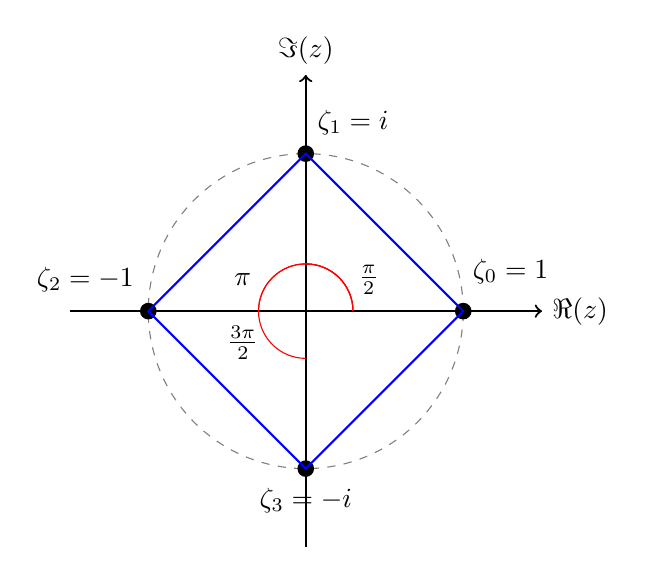
\begin{tikzpicture}[scale=2]
% Draw axes
\draw[->, thick] (-1.5,0) -- (1.5,0) node[right] {$\Re(z)$};
\draw[->, thick] (0,-1.5) -- (0,1.5) node[above] {$\Im(z)$};

% Draw unit circle
\draw[gray,dashed] (0,0) circle (1);

% Draw fourth roots of unity
\fill (1,0) circle (1.5pt);
\fill (0,1) circle (1.5pt);
\fill (-1,0) circle (1.5pt);
\fill (0,-1) circle (1.5pt);

% Connect points to form square
\draw[blue, thick] (1,0) -- (0,1) -- (-1,0) -- (0,-1) -- cycle;

% Add angles
\draw[red] (0.3,0) arc (0:90:0.3);
\draw[red] (0.3,0) arc (0:180:0.3);
\draw[red] (0.3,0) arc (0:270:0.3);

% Label angles
\node at (0.4,0.2) {$\frac{\pi}{2}$};
\node at (-0.4,0.2) {$\pi$};
\node at (-0.4,-0.2) {$\frac{3\pi}{2}$};

% Movable labels for roots of unity (adjust coordinates as needed)
\node at (1.3,0.25) {$\zeta_0 = 1$};
\node at (0.3,1.2) {$\zeta_1 = i$};
\node at (-1.4,0.2) {$\zeta_2 = -1$};
\node at (0,-1.2) {$\zeta_3 = -i$};

\end{tikzpicture}
\caption{\textit{The fourth roots of unity form a square in the complex plane, with vertices equally spaced around the unit circle.}}
\label{fig:fourth-roots}
\end{figure}



\noindent More generally, for any complex number $z = re^{i\theta}$, its $n$th roots are given by:
\[
w_k = \sqrt[n]{r}e^{i(\theta + 2\pi k)/n}, \quad k = 0,1,\ldots,n-1
\]

\noindent This formula has a beautiful geometric interpretation:
\begin{itemize}
   \item $\sqrt[n]{r}$ determines the distance of all roots from the origin
   \item The angles $\frac{\theta + 2\pi k}{n}$ space the roots evenly around a circle
   \item The roots form a regular $n$-gon in the complex plane
\end{itemize}

\begin{figure}[H]
\centering
\begin{tikzpicture}[scale=2]
% Draw axes
\draw[->] (-1.5,0) -- (1.5,0) node[right] {$\Re(z)$};
\draw[->] (0,-1.5) -- (0,1.5) node[above] {$\Im(z)$};

% Draw unit circle
\draw[gray,dashed] (0,0) circle (1);

% Draw sixth roots of unity
\foreach \k in {0,1,2,3,4,5} {
   \pgfmathsetmacro{\angle}{60*\k}
   \pgfmathsetmacro{\x}{cos(\angle)}
   \pgfmathsetmacro{\y}{sin(\angle)}
   \fill (\x,\y) circle (1pt);
   \draw[blue] (\x,\y) -- ({\x+0.2*cos(\angle+120)},{\y+0.2*sin(\angle+120)});
}

% Connect points to form hexagon
\draw[blue] (1,0) -- ({cos(60)},{sin(60)}) -- ({cos(120)},{sin(120)}) --
   ({cos(180)},{sin(180)}) -- ({cos(240)},{sin(240)}) -- ({cos(300)},{sin(300)}) -- cycle;

% Label some points
\node[right] at (1,0) {$1$};
\node[above] at ({cos(60)},{sin(60)}) {$\omega$};
\node[left] at (-1,0) {$\omega^3$};
\end{tikzpicture}
\caption{\textit{The sixth roots of unity form a regular hexagon in the complex plane. Here $\omega = e^{2\pi i/6}$ is a primitive sixth root of unity.}}
\label{fig:sixth-roots}
\end{figure}

\noindent The roots of unity play a crucial role in many areas of mathematics:
\begin{itemize}
   \item They are key to understanding cyclotomic polynomials
   \item They appear in the Fast Fourier Transform algorithm
   \item They help solve equations like $x^n = 1$
   \item They provide symmetries for geometric constructions
\end{itemize}
\index{Primitive Root}
\noindent A particularly important concept is that of a \textbf{primitive root of unity}. A complex number $\omega$ is called a primitive $n$th root of unity if:
\begin{itemize}
   \item $\omega^n = 1$
   \item $\omega^k \neq 1$ for all $1 \leq k < n$
\end{itemize}

\noindent For example, if $\omega = e^{2\pi i/6}$, then $\{\omega, \omega^5\}$ are the primitive sixth roots of unity, while $\{1, \omega^2, \omega^3, \omega^4\}$ are not primitive (they are also roots of unity of smaller orders).

\begin{figure}[H]
\centering
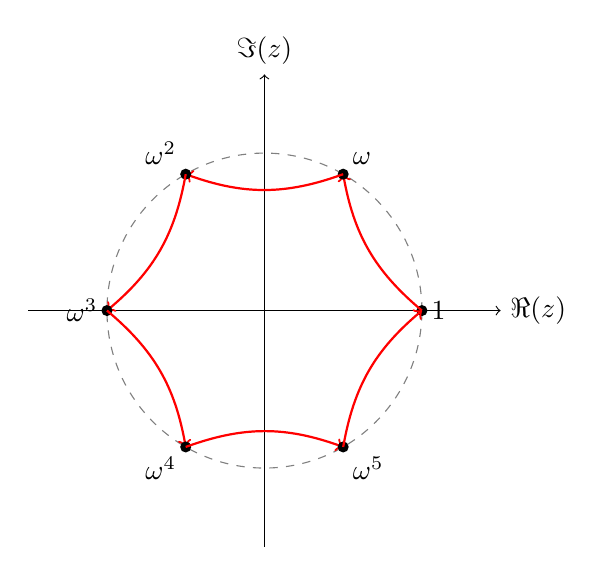
\begin{tikzpicture}[scale=2]
% Draw axes
\draw[->] (-1.5,0) -- (1.5,0) node[right] {$\Re(z)$};
\draw[->] (0,-1.5) -- (0,1.5) node[above] {$\Im(z)$};

% Draw unit circle
\draw[gray,dashed] (0,0) circle (1);

% Draw powers of a primitive sixth root
\foreach \k in {0,1,2,3,4,5} {
   \pgfmathsetmacro{\angle}{60*\k}
   \pgfmathsetmacro{\x}{cos(\angle)}
   \pgfmathsetmacro{\y}{sin(\angle)}
   
   % Draw points
   \fill (\x,\y) circle (1pt);
   
   % Draw arrows connecting consecutive powers
   \pgfmathsetmacro{\nextangle}{60*mod(\k+1,6)}
   \pgfmathsetmacro{\nextx}{cos(\nextangle)}
   \pgfmathsetmacro{\nexty}{sin(\nextangle)}
   \draw[->, red, thick] (\x,\y) to[bend left=20] (\nextx,\nexty);
}

% Label points
\node[right] at (1,0) {$1$};
\node[above right] at ({cos(60)},{sin(60)}) {$\omega$};
\node[above left] at ({cos(120)},{sin(120)}) {$\omega^2$};
\node[left] at (-1,0) {$\omega^3$};
\node[below left] at ({cos(240)},{sin(240)}) {$\omega^4$};
\node[below right] at ({cos(300)},{sin(300)}) {$\omega^5$};

\end{tikzpicture}
\caption{\textit{Powers of a primitive sixth root of unity $\omega = e^{2\pi i/6}$. The arrows show how multiplication by $\omega$ cycles through all sixth roots before returning to 1.}}
\label{fig:primitive-roots}
\end{figure}

\noindent De Moivre's theorem and roots of unity demonstrate how deeply intertwined complex numbers are with both algebra and geometry. The regular polygons formed by roots of unity reveal symmetries that would be hidden in purely algebraic manipulations, while the polar form makes clear why these symmetries exist in the first place.


\exampleline
\begin{example}
Find all values of $(-8)^{1/3}$ in the complex plane, expressing them both in polar and rectangular form. Which of these is the principal cube root?

\begin{solution}
Let's solve this step by step using the polar representation of complex numbers.

\begin{enumerate}
\item First, write -8 in polar form:
  \begin{align*}
  -8 &= 8e^{i\pi} \quad \text{(since -8 lies on the negative real axis)}
  \end{align*}

\item To find the cube roots, we use the formula:
  \[
  w_k = \sqrt[3]{r}e^{i(\theta + 2\pi k)/3}, \quad k = 0,1,2
  \]
  where $r = 8$ and $\theta = \pi$

\item Calculate $\sqrt[3]{r} = 2$ and substitute:
  \begin{align*}
  w_k &= 2e^{i(\pi + 2\pi k)/3} \quad k = 0,1,2 \\
  &= 2e^{i\pi(1 + 2k)/3}
  \end{align*}

\item Calculate each root for $k = 0,1,2$:
  \begin{align*}
  w_0 &= 2e^{i\pi/3} = 2(\cos(\pi/3) + i\sin(\pi/3)) = 1 + i\sqrt{3} \\
  w_1 &= 2e^{i\pi} = -2 \\
  w_2 &= 2e^{5i\pi/3} = 2(\cos(5\pi/3) + i\sin(5\pi/3)) = 1 - i\sqrt{3}
  \end{align*}

\item The principal cube root is the one with argument in $[-\pi/3, \pi/3)$. Here, that's $w_1 = -2$.
\end{enumerate}

\begin{figure}[H]
\centering
\begin{tikzpicture}[scale=1]
% Draw axes
\draw[->] (-3,0) -- (3,0) node[right] {$\Re(z)$};
\draw[->] (0,-3) -- (0,3) node[above] {$\Im(z)$};

% Draw points
\fill (1,1.732) circle (2pt) node[above right] {$1+i\sqrt{3}$};
\fill (-2,0) circle (2pt) node[left] {$-2$};
\fill (1,-1.732) circle (2pt) node[below right] {$1-i\sqrt{3}$};

% Draw rays from origin
\draw[blue,dashed] (0,0) -- (1,1.732);
\draw[blue,dashed] (0,0) -- (-2,0);
\draw[blue,dashed] (0,0) -- (1,-1.732);

% Add angles
\draw[red] (0.7,0) arc (0:60:0.7);
\draw[red] (0.7,0) arc (0:180:0.7);
\draw[red] (0.7,0) arc (0:300:0.7);

% Label angles
\node at (0.8,0.4) {$\frac{\pi}{3}$};
\node at (-0.8,0.4) {$\pi$};
\node at (0.8,-0.4) {$\frac{5\pi}{3}$};
\end{tikzpicture}
\caption{\textit{The three cube roots of -8 form an equilateral triangle when scaled to show their relative positions.}}
\end{figure}
\end{solution}
\end{example}
\exampleline
\begin{example}
Find all primitive roots of $z^4 - 1 = 0$, explaining why each root is or is not primitive.

\begin{solution}
Let's solve this systematically.

\begin{enumerate}
\item First, find all fourth roots of unity. Using $\zeta_k = e^{2\pi i k/4}$ for $k = 0,1,2,3$:
  \begin{align*}
  \zeta_0 &= 1 = 1 + 0i \\
  \zeta_1 &= i = 0 + i \\
  \zeta_2 &= -1 = -1 + 0i \\
  \zeta_3 &= -i = 0 - i
  \end{align*}

\item To determine which roots are primitive, we must check the powers of each root:
  
\item For $\zeta_1 = i$:
  \begin{align*}
  i^1 &= i \\
  i^2 &= -1 \\
  i^3 &= -i \\
  i^4 &= 1
  \end{align*}
  Since no smaller power equals 1, $i$ is primitive.

\item For $\zeta_2 = -1$:
  \begin{align*}
  (-1)^1 &= -1 \\
  (-1)^2 &= 1
  \end{align*}
  Not primitive as it's a solution to $z^2 = 1$.

\item For $\zeta_3 = -i$:
  \begin{align*}
  (-i)^1 &= -i \\
  (-i)^2 &= -1 \\
  (-i)^3 &= i \\
  (-i)^4 &= 1
  \end{align*}
  Since no smaller power equals 1, $-i$ is primitive.

\item Therefore, the primitive fourth roots of unity are $i$ and $-i$.

\end{enumerate}

\begin{figure}[H]
\centering
\begin{tikzpicture}[scale=2]
  % Macro: #1 = point coordinate, #2 = label offset, #3 = label text.
  \newcommand{\drawLabeledPoint}[3]{%
    \fill (#1) circle (1pt);
    \node at ($ (#1) + (#2) $) {#3};
  }

% Draw axes
\draw[->] (-1.5,0) -- (1.5,0) node[right] {$\Re(z)$};
\draw[->] (0,-1.5) -- (0,1.5) node[above] {$\Im(z)$};

% Draw unit circle
\draw[gray,dashed] (0,0) circle (1);

% Draw points
  \drawLabeledPoint{1,0}{0.2,0.1}   {$1$}
  \drawLabeledPoint{0,1}{0.1,0.3}   {$i$}
  \drawLabeledPoint{-1,0}{-0.3,0.1} {$-1$}
  \drawLabeledPoint{0,-1}{0.1,-0.3} {$-i$}

% Mark primitive roots in different color
\draw[red,thick] (0,1) circle (2pt);
\draw[red,thick] (0,-1) circle (2pt);

% Add labels for cyclic subgroups
\draw[blue,->] (0.3,0.3) arc (45:135:0.4) node[above] {$\times i$};
\draw[blue,->] (-0.3,0.3) arc (135:225:0.4) node[left] {$\times i$};
\draw[blue,->] (-0.3,-0.3) arc (225:315:0.4) node[below] {$\times i$};
\draw[blue,->] (0.3,-0.3) arc (-45:45:0.4) node[right] {$\times i$};

\end{tikzpicture}
\caption{\textit{The fourth roots of unity. The primitive roots (circled in red) generate all other roots through repeated multiplication.}}
\end{figure}

\noindent As shown in the diagram, multiplying by a primitive root ($i$ or $-i$) cycles through all four roots before returning to 1, while multiplying by the non-primitive root $-1$ only cycles through two values.
\end{solution}
\end{example}
\exampleline

\subsection*{Fundamental Theorem of Algebra} \index{Fundamental Theorem of Algebra}

\noindent Our journey through complex roots and De Moivre's theorem leads us naturally to one of the most profound results in mathematics: the \textbf{Fundamental Theorem of Algebra}. This theorem states that every non-constant polynomial with complex coefficients has at least one complex root. While its statement is remarkably simple, its implications are far-reaching. \\

\noindent To appreciate the power of this theorem, let's consider what it tells us. Given any polynomial:
\[
p(z) = a_nz^n + a_{n-1}z^{n-1} + \cdots + a_1z + a_0
\]
where $a_n \neq 0$ and the coefficients $a_k$ are complex numbers, there exists at least one complex number $c$ such that $p(c) = 0$. \\

\noindent But the theorem tells us much more. Once we find one root $c_1$, we can factor out $(z-c_1)$:
\[
p(z) = (z-c_1)(a_nz^{n-1} + b_{n-2}z^{n-2} + \cdots + b_1z + b_0)
\]

\noindent The remaining factor is still a polynomial with complex coefficients, so the theorem applies again. This process continues until we have found all $n$ roots (counting multiplicity):
\[
p(z) = a_n(z-c_1)(z-c_2)\cdots(z-c_n)
\]

\noindent This complete factorization has several profound implications:
\begin{itemize}
   \item Every polynomial of degree $n$ has exactly $n$ complex roots (counting multiplicity)
   \item There's no need to invent new kinds of numbers to solve polynomial equations
   \item The complex numbers form an algebraically closed field
\end{itemize}

\noindent The connection to our previous study of roots of unity becomes clear when we consider the equation $z^n - 1 = 0$. The Fundamental Theorem guarantees that this equation has exactly $n$ solutions, and De Moivre's theorem shows us they are:
\[
\zeta_k = e^{2\pi i k/n}, \quad k = 0,1,\ldots,n-1
\]

\noindent More generally, for any complex number $w$, the equation $z^n = w$ has exactly $n$ solutions:
\[
z_k = \sqrt[n]{|w|}e^{i(\arg(w) + 2\pi k)/n}, \quad k = 0,1,\ldots,n-1
\]

\noindent The completeness of complex numbers stands in stark contrast to the real numbers $\mathbb{R}$. Consider these examples:
\begin{itemize}
   \item In $\mathbb{R}$: $x^2 + 1 = 0$ has no solutions
   \item In $\mathbb{C}$: $z^2 + 1 = 0$ has two solutions: $i$ and $-i$
   \item In $\mathbb{R}$: $x^4 - 2x^2 + 2 = 0$ has no solutions
   \item In $\mathbb{C}$: $z^4 - 2z^2 + 2 = (z^2-1+i)(z^2-1-i)$ has four solutions
\end{itemize}

\noindent While there are larger number systems that contain $\mathbb{C}$ (such as the quaternions $\mathbb{H}$ or the octonions $\mathbb{O}$), they necessarily sacrifice some of the nice properties of complex arithmetic:
\begin{itemize}
   \item Quaternions lose commutativity of multiplication ($ij \neq ji$)
   \item Octonions lose both commutativity and associativity
   \item Neither system admits an ordering compatible with their operations
\end{itemize}

\noindent This makes $\mathbb{C}$ a sort of ``sweet spot" in mathematics—large enough to solve all polynomial equations, yet well-behaved enough to maintain the familiar rules of arithmetic. The Fundamental Theorem of Algebra thus marks complex numbers as both complete and minimal: they are exactly what we need to do algebra, no more and no less.

\newpage












\lecture{Complex Functions} \index{Complex Functions}

\noindent Complex functions extend the ideas of real-valued functions into the complex plane, revealing deep connections between algebra and geometry. Unlike real functions, which map points on a line to other points on a line, complex functions transform entire regions of the plane, often producing intricate and elegant geometric structures. These functions play a crucial role in various mathematical fields, offering insights into both theoretical and applied problems.

\subsection*{The Nature of Complex Functions} \index{Complex Function Definition}

\noindent A complex function $f$ is a rule that assigns to each complex number $z$ in some domain $D \subseteq \mathbb{C}$ another complex number $w = f(z)$. Since both input and output are complex numbers, we can write:
\[
f: D \rightarrow \mathbb{C}, \quad z \mapsto w = f(z)
\]

\noindent Because complex numbers can be written in the form $z = x + yi$, every complex function can be expressed in terms of two real-valued functions $u(x,y)$ and $v(x,y)$:
\[
f(z) = f(x + yi) = u(x,y) + iv(x,y)
\]

\noindent This representation, splitting a complex function into its real and imaginary parts, provides a bridge between complex analysis and multivariable calculus. The functions $u$ and $v$ are called the \textbf{component functions} of $f$. \\

\noindent The behavior of complex functions differs fundamentally from real functions in several ways. When we extend a real function to the complex plane, new phenomena emerge. Consider these key differences:

\begin{itemize}
    \item A complex function $f(z)$ actually maps points from a plane to another plane, making it inherently two-dimensional in both its domain and range
    \item The presence of $i$ introduces a rotational aspect to function behavior that has no real-valued analog
    \item Even simple functions like $f(z) = z^2$ exhibit richer geometric properties than their real counterparts
\end{itemize}

\noindent For example, consider the function $f(z) = z^2$. Writing $z = x + yi$:
\begin{align*}
f(z) &= (x + yi)^2 \\
&= x^2 - y^2 + (2xy)i
\end{align*}
Here, $u(x,y) = x^2 - y^2$ and $v(x,y) = 2xy$. \\

\noindent The interaction between the real and imaginary parts creates interesting geometric effects. When we square a complex number:
\begin{itemize}
    \item The function doubles the argument (angle) of the input: $\arg(z^2) = 2\arg(z)$
    \item The magnitude is squared: $|z^2| = |z|^2$
    \item Points on the unit circle $|z| = 1$ map to points on the unit circle, but they travel twice as far around it
\end{itemize}

\noindent This geometric behavior contrasts sharply with real functions. When we square a real number, we only see magnitude changes—the geometric aspect of angle doubling is completely hidden in the real case. \\

\noindent Even familiar operations take on new meaning. Consider multiplication by $i$:
\begin{align*}
i(x + yi) &= ix - y \\
&= -y + xi
\end{align*}

\noindent This simple operation rotates every point in the complex plane by 90 degrees counterclockwise about the origin. No real-valued function can capture this rotational behavior, highlighting how complex functions incorporate both algebraic and geometric transformations simultaneously. \\

\noindent The real and imaginary component functions $u$ and $v$ are not independent—they are intimately connected through the properties of complex differentiation, as we'll discover when we study the Cauchy-Riemann equations. This interplay between components gives complex functions their distinctive properties and leads to powerful theorems with no real-valued analogues.

\subsection*{Domain and Range Considerations} \index{Complex Domain}

\noindent The domain of a complex function requires careful consideration. While real functions might be restricted by operations like division by zero or taking square roots of negative numbers, complex functions often have broader domains. However, certain functions exhibit multi-valued behavior in the complex plane, necessitating special handling. For instance:

\begin{itemize}
\item $\sqrt{z}$ is defined for all complex numbers except $z = 0$, though it requires a branch cut to make it single-valued.
\item $\ln(z)$ is defined for all nonzero complex numbers, but since logarithms of complex numbers involve arguments that can wrap around $2\pi$, a branch cut is needed to maintain consistency.
\item $\frac{1}{z}$ is defined for all complex numbers except $z = 0$, with no need for a branch cut since it does not exhibit multi-valued behavior.
\end{itemize}

\noindent In cases where a function is naturally multi-valued, a \textbf{branch cut} is introduced to restrict its domain to a single-valued region. A branch cut is a deliberate discontinuity in the complex plane that defines a consistent way to evaluate the function. We will discuss this concept in more detail in the following paragraphs. \\

\noindent The concept of \textbf{natural domain} extends to complex functions: it's the largest subset of $\mathbb{C}$ where the function can be meaningfully defined. However, we often restrict the domain further to ensure nice properties like continuity or differentiability.


\subsection*{Elementary Complex Functions} \index{Elementary Complex Functions}

\noindent The extension of elementary functions to the complex domain reveals surprising depth and beauty. Let's examine each class:

\subsubsection*{Polynomial and Rational Functions}

\noindent Complex polynomials greet us as the most approachable extension from real calculus into the vast plane of $\mathbb{C}$, offering a smooth transition from the multivariable mappings we’ve explored to the intricate world of complex numbers. They take the familiar form:
\[
P(z) = a_n z^n + a_{n-1} z^{n-1} + \cdots + a_1 z + a_0,
\]
where the coefficients $a_k$ are complex numbers, and $a_n \neq 0$ sets the degree $n$. These functions are defined everywhere in $\mathbb{C}$, a testament to their well-mannered nature. With no division or roots to restrict them, polynomials operate seamlessly across the plane, free of the gaps or breaks that other functions might encounter. This universality comes from their reliance on addition and multiplication—operations that never falter in the complex realm—making them a steady foundation as we venture deeper. \\

\noindent Their simplicity hides a profound truth: every non-constant polynomial has roots in $\mathbb{C}$, a fact we’ll call upon often. For instance, take $P(z) = z^2 - 2z + 2$. Factoring yields:
\[
P(z) = (z - 1 - i)(z - 1 + i),
\]
with roots at $z = 1 + i$ and $z = 1 - i$, ensuring the degree (2) matches the number of roots when counted appropriately. As $z$ roams far from the origin, the leading term $a_n z^n$ takes charge; for $P(z) = z^2 - 2z + 2$, as $|z| \to \infty$, $|P(z)| \approx |z|^2 \to \infty$, stretching magnitudes skyward while angles twist twice around the plane—a geometric flair we’ll visualize later. \\

\noindent Rational functions, born from the quotient of polynomials:
\[
R(z) = \frac{P(z)}{Q(z)},
\]
shift the narrative by introducing points of drama—places where $Q(z) = 0$. These are the \textbf{poles}, spots where the function surges to infinity, breaking the calm expanse of polynomials. Consider $R(z) = \frac{z + 1}{z - 2}$. The pole at $z = 2$ marks where the denominator vanishes, and as $z$ nears 2, say at $z = 2.01$:
\[
R(2.01) = \frac{2.01 + 1}{2.01 - 2} = \frac{3.01}{0.01} = 301,
\]
a sharp climb that hints at the pole’s power. The \textbf{order of a pole} at $z_0$ tells us how fiercely this happens. If $Q(z) = (z - z_0)^m Q'(z)$, where $Q'(z_0) \neq 0$, the pole has order $m$. A \textbf{simple pole} (order 1) grows linearly in $1/|z - z_0|$, while \textbf{multiple poles} (order $m > 1$) amplify this ascent. For $R(z) = \frac{1}{(z - 1)^2}$, the pole at $z = 1$ is order 2:
\[
R(1.01) = \frac{1}{(0.01)^2} = \frac{1}{0.0001} = 10000,
\]
a quadratic leap compared to a simple pole’s gentler rise. \\

\noindent This interplay of order shapes the function’s behavior near singularities. Picture $R(z) = \frac{z}{(z + i)^3 (z - i)}$: it has a triple pole at $z = -i$ and a simple pole at $z = i$. Near $z = -i + 0.01$:
\[
R(-i + 0.01) \approx \frac{-i + 0.01}{(0.01)^3 (0.01 - i)} \approx \frac{-i}{0.0001 \cdot (-i)} = \frac{1}{0.0001} = 10000,
\]
\noindent dominated by the triple pole’s cubic surge. The following diagram captures this landscape:

\begin{figure}[H]
  \centering
\begin{tikzpicture}
    \draw[thick,->] (-3,0) -- (3,0) node[right] {$\Re(z)$};
    \draw[thick,->] (0,-3) -- (0,3) node[above] {$\Im(z)$};
    
    % Simple poles
    \filldraw[red] (-1.5,1) circle (2pt) node[above] {\footnotesize $-1.5 + i$};
    \filldraw[red] (1,-1) circle (2pt) node[below] {\footnotesize $1 - i$};
    
    % Double pole
    \draw[blue,thick] (0.5,1.5) circle (3pt);
    \filldraw[blue] (0.5,1.5) circle (2pt);
    \node[right] at (0.5,1.5) {\footnotesize $0.5 + 1.5i$ (order 2)};
    
    % Triple pole
    \draw[green,thick] (-2,-1.5) circle (4pt);
    \draw[green,thick] (-2,-1.5) circle (3pt);
    \filldraw[green] (-2,-1.5) circle (2pt);
    \node[below left] at (-2,-1.5) {\footnotesize $-2 - 1.5i$ (order 3)};
    
    % Legend
    \node[right] at (3,-2) {\textcolor{red}{\(\bullet\) Simple pole}};
    \node[right] at (3,-2.5) {\textcolor{blue}{\(\circ\) Order 2 pole}};
    \node[right] at (3,-3) {\textcolor{green}{\(\circ\) Order 3 pole}};
\end{tikzpicture}
\caption{\textit{Poles of a rational function, with simple poles (red dots) at $-1.5 + i$ and $1 - i$, a double pole (blue ring) at $0.5 + 1.5i$, and a triple pole (green rings) at $-2 - 1.5i$.}}
\label{fig:pole-orders}

\end{figure}

\noindent The diagram paints a vivid scene: simple poles at $-1.5 + i$ and $1 - i$ rise steadily, the double pole at $0.5 + 1.5i$ accelerates quadratically, and the triple pole at $-2 - 1.5i$ soars cubically, each order sculpting the function’s climb. Polynomials, in contrast, stretch outward without such interruptions, their roots quietly anchoring the plane while their growth at infinity hints at a rotational twist—$P(z) = z^3$ triples angles as magnitudes cube, a preview of mapping wonders to come.

\exampleline
\begin{example}
Identify the poles and their orders for $R(z) = \frac{z^2 + 1}{(z - 1)^2 (z + 2)}$, and describe the behavior near $z = 1$.

\begin{solution}
Set the denominator to zero: $(z - 1)^2 (z + 2) = 0$, giving poles at $z = 1$ (order 2) and $z = -2$ (order 1). The numerator $z^2 + 1$ is nonzero at both ($1^2 + 1 = 2$, $(-2)^2 + 1 = 5$), confirming these as poles. Near $z = 1$, let $z = 1 + h$ with small $h$:
\[
R(1 + h) = \frac{(1 + h)^2 + 1}{h^2 (1 + h + 2)} = \frac{1 + 2h + h^2 + 1}{h^2 (3 + h)} = \frac{2 + 2h + h^2}{h^2 (3 + h)}.
\]
For $h = 0.01$:
\[
R(1.01) = \frac{2 + 0.02 + 0.0001}{0.0001 \cdot 3.01} \approx \frac{2.0201}{0.000301} \approx 6711,
\]
a rapid quadratic growth ($|R| \propto 1/h^2$) due to the double pole, far steeper than a simple pole’s linear rise.
\end{solution}
\end{example}
\exampleline

\noindent Polynomials and rational functions thus offer a dual tale: the steady reach of polynomials across $\mathbb{C}$, punctuated by roots and infinite growth, versus the dramatic peaks of rational functions at their poles, each shaping the complex plane in distinct, vivid ways.

\subsubsection*{Exponential Function} \index{Complex Exponential}

\noindent The exponential function, a cornerstone of real calculus, unfurls into a marvel of complexity and elegance when we extend it into the complex plane, revealing a tapestry of growth, rotation, and periodicity that transcends its real origins. In $\mathbb{R}$, $e^x$ is a relentless climber, always positive and surging toward infinity as $x$ grows. In $\mathbb{C}$, it becomes a dancer across the plane, guided by Euler’s formula, which breathes life into its complex form:
\[
e^z = e^{x + yi} = e^x (\cos y + i \sin y).
\]
Here, $z = x + yi$ splits into a real part $x$ that dictates magnitude and an imaginary part $y$ that spins the output around the unit circle, marrying exponential growth with trigonometric oscillation. This definition, elegant in its simplicity, preserves the sacred property of exponents we know so well: $e^{z_1 + z_2} = e^{z_1} e^{z_2}$. For $z_1 = 1 + i$ and $z_2 = 2 - i$:
\[
e^{(1 + i) + (2 - i)} = e^{3} = e^3 (\cos 0 + i \sin 0) = e^3,
\]
while separately:
\[
e^{1 + i} e^{2 - i} = e^1 (\cos 1 + i \sin 1) \cdot e^2 (\cos (-1) + i \sin (-1))
\]
\[
 = e^3 (\cos 1 \cos (-1) + i \sin 1 \cos (-1) + i \cos 1 \sin (-1) - \sin 1 \sin (-1)),
\]
and since $\cos(-1) = \cos 1$, $\sin(-1) = -\sin 1$, this simplifies to $e^3 (\cos^2 1 + \sin^2 1) = e^3$, a harmony unbroken across $\mathbb{C}$. \\

\noindent This extension unveils a function that is \textbf{entire}—defined and complex-differentiable for all $z \in \mathbb{C}$—a trait it shares with polynomials, free of the singularities that haunt rational functions. Compute $e^{2 + 3i}$:
\[
e^{2 + 3i} = e^2 (\cos 3 + i \sin 3),
\]
a point in the plane whose magnitude $e^2$ reflects $x = 2$, and whose argument $3$ radians (about 171.9°) reflects $y = 3$, reachable with any complex input. Unlike its real sibling, which never dips below zero, the complex exponential never rests at zero: $|e^z| = e^x > 0$, and its range is $\mathbb{C} \setminus \{0\}$. Try $e^{0 + i\pi} = \cos \pi + i \sin \pi = -1$, a negative real number, impossible in $\mathbb{R}$. \\

\noindent A mesmerizing property emerges in the imaginary direction: periodicity. Since $e^{i 2\pi} = \cos 2\pi + i \sin 2\pi = 1$, we find:
\[
e^{z + 2\pi i} = e^z e^{2\pi i} = e^z \cdot 1 = e^z,
\]
a period of $2\pi i$ along the imaginary axis, a cycle absent in real exponentials. This periodicity mirrors the circular motion of $\cos y + i \sin y$, tying the function to the geometry of the unit circle. For $z = x + i y$, as $y$ increases by $2\pi$, the output loops back, tracing a spiral when $x$ varies—a dynamic we’ll visualize. \\

\noindent The exponential’s mapping properties deepen its allure. Consider $z = x + i y$ as a point in the $z$-plane. The real part $x$ controls growth ($|e^z| = e^x$), while $y$ dictates rotation ($\arg(e^z) = y$). Horizontal lines $y = c$ map to rays from the origin at angle $c$, since $e^{x + i c} = e^x e^{i c}$, with magnitude $e^x$ stretching from 0 to $\infty$. Vertical lines $x = c$ map to circles $|w| = e^c$, as $e^{c + i y} = e^c (\cos y + i \sin y)$ traces the circle of radius $e^c$. This transformation from Cartesian strips to polar rays and circles is a hallmark of the complex exponential, connecting to polar coordinates in a way real exponentials cannot. \\

\begin{figure}[H]
  \centering
  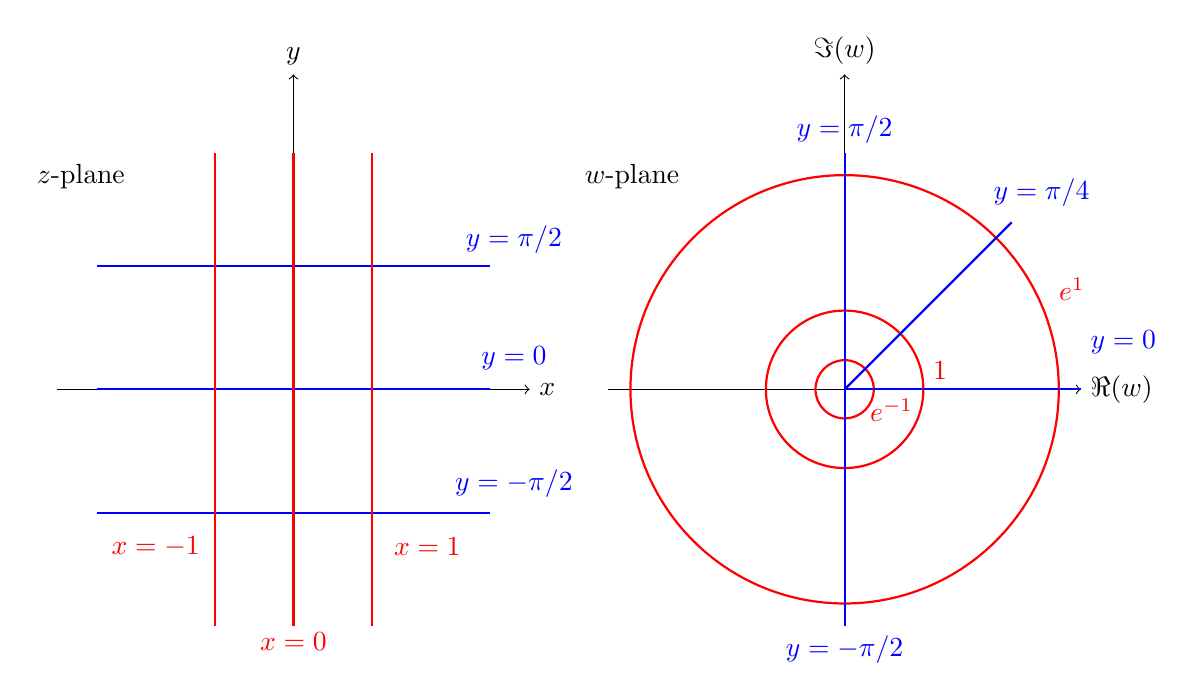
\begin{tikzpicture}[scale=1]
    %%%%%%%%%%%%%%%%%%%%%%%%%%%%%%%%%%%%%%%%%%%%%%
    % Left: Domain (z-plane)
    %%%%%%%%%%%%%%%%%%%%%%%%%%%%%%%%%%%%%%%%%%%%%%
    \begin{scope}
      % Axes
      \draw[->] (-3,0) -- (3,0) node[right] {$x$};
      \draw[->] (0,-3) -- (0,4) node[above] {$y$};
      \node at (-2.7,2.7) {$z$-plane};

      % Horizontal lines: y = -π/2, 0, π/2 (in blue)
      \draw[blue, thick, domain=-2.5:2.5] plot (\x, {0});
      \draw[blue, thick, domain=-2.5:2.5] plot (\x, {1.57});
      \draw[blue, thick, domain=-2.5:2.5] plot (\x, {-1.57});
      \node[blue] at (2.8,0.4) {$y=0$};
      \node[blue] at (2.8,1.9) {$y=\pi/2$};
      \node[blue] at (2.8,-1.2) {$y=-\pi/2$};

      % Vertical lines: x = -1, 0, 1 (in red)
      \draw[red, thick, domain=-3:3] plot ({-1}, \x);
      \draw[red, thick, domain=-3:3] plot ({0}, \x);
      \draw[red, thick, domain=-3:3] plot ({1}, \x);
      \node[red] at (-1.75,-2) {$x=-1$};
      \node[red] at (0,-3.2) {$x=0$};
      \node[red] at (1.7,-2) {$x=1$};
    \end{scope}

    %%%%%%%%%%%%%%%%%%%%%%%%%%%%%%%%%%%%%%%%%%%%%%
    % Right: Image (w-plane), mapping via w = e^z.
    %         Vertical lines -> circles; Horizontal lines -> rays.
    %%%%%%%%%%%%%%%%%%%%%%%%%%%%%%%%%%%%%%%%%%%%%%
    \begin{scope}[xshift=7cm]
      % Axes
      \draw[->] (-3,0) -- (3,0) node[right] {$\Re(w)$};
      \draw[->] (0,-3) -- (0,4) node[above] {$\Im(w)$};
      \node at (-2.7,2.7) {$w$-plane};

      % Vertical lines: x=c map to circles |w| = e^c.
      % For c = -1, 0, 1 -> radii: e^{-1} ≈ 0.37, 1, e^{1} ≈ 2.72.
      \draw[red, thick] (0,0) circle (0.37);
      \node[red] at (0.2,0) [below right] {$e^{-1}$};
      \draw[red, thick] (0,0) circle (1);
      \node[red] at (1,0) [above right] {$1$};
      \draw[red, thick] (0,0) circle (2.72);
      \node[red] at (2.6,1) [above right] {$e^{1}$};

      % Horizontal lines: y=c map to rays (angle = c).
      % Draw rays for y = -π/2, 0, π/2.
      \draw[blue, thick, domain=0:3] plot ({\x*cos(0)},{\x*sin(0)});
      \node[blue] at (3,0.6) [right] {$y=0$};
      \draw[blue, thick, domain=0:3] plot ({\x*cos(90)},{\x*sin(90)});
      \node[blue] at (0,3) [above] {$y=\pi/2$};
      \draw[blue, thick, domain=0:3] plot ({\x*cos(-90)},{\x*sin(-90)});
      \node[blue] at (0,-3) [below] {$y=-\pi/2$};

      % Additional example: ray for y = π/4.
      \draw[blue, thick, domain=0:3] plot ({\x*cos(45)},{\x*sin(45)});
      \node[blue] at (2.5,2.5) {$y=\pi/4$};
    \end{scope}
  \end{tikzpicture}
  \caption{Mapping of the complex exponential $w=e^z$. Horizontal lines in the $z$-plane ($y=$ constant) map to rays in the $w$-plane, and vertical lines ($x=$ constant) map to circles of radius $e^x$.}
  \label{fig:exp-mapping}
\end{figure}

\noindent Its growth rate further distinguishes it. In $\mathbb{R}$, $e^x$ outpaces polynomials; in $\mathbb{C}$, this persists, but direction matters. Along the real axis ($y = 0$), $|e^x| = e^x \to \infty$ as $x \to \infty$. Along the imaginary axis ($x = 0$), $e^{i y} = \cos y + i \sin y$ stays on the unit circle, $|e^{i y}| = 1$. In general directions, $|e^{x + i y}| = e^x$ grows or decays with $x$, while $y$ spins the phase—a balance of magnitude and motion. \\

\noindent This function’s unity with trigonometric functions, via Euler’s formula, is profound. Since $e^{i y} = \cos y + i \sin y$ and $e^{-i y} = \cos y - i \sin y$, we derive:
\[
\cos y = \frac{e^{i y} + e^{-i y}}{2}, \quad \sin y = \frac{e^{i y} - e^{-i y}}{2i},
\]
a bridge we’ll cross in the next subsection. For $z = i\pi/4$:
\[
e^{i \pi/4} = \cos \frac{\pi}{4} + i \sin \frac{\pi}{4} = \frac{\sqrt{2}}{2} + i \frac{\sqrt{2}}{2},
\]
a point at 45°, effortlessly computed.

\begin{figure}[H]
\centering
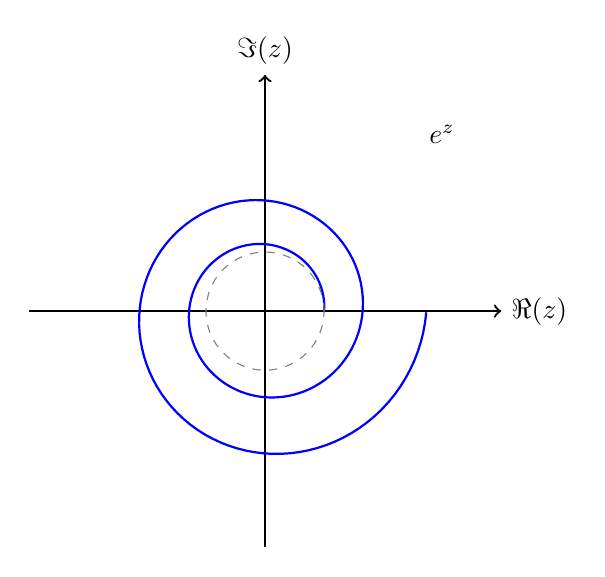
\begin{tikzpicture}[scale=1.5]
  % Axes
  \draw[->, thick] (-2,0) -- (2,0) node[right] {$\Re(z)$};
  \draw[->, thick] (0,-2) -- (0,2) node[above] {$\Im(z)$};
  
  % Spiral for e^z
  \draw[blue, thick] plot[domain=0:12.56, samples=200] ({0.5*exp(0.08*\x)*cos(deg(\x))},{0.5*exp(0.08*\x)*sin(deg(\x))});
  \node at (1.5,1.5) {$e^z$};
  \draw[gray, dashed] (0,0) circle (0.5);
\end{tikzpicture}
\caption{\textit{The complex exponential $e^z$ maps a strip to a spiral, growing with real part $x$ and cycling with imaginary part $y$, orbiting the unit circle (dashed).}}
\label{fig:exp-spiral}
\end{figure}

\noindent The exponential’s role in visualization is pivotal. Its periodicity and growth make it a lens for periodic phenomena—like waves or rotations—in $\mathbb{C}$, a tool we’ll wield in mapping diagrams. For $z = -1 + i 2\pi$:
\[
e^{-1 + i 2\pi} = e^{-1} (\cos 2\pi + i \sin 2\pi) = e^{-1} \approx 0.367,
\]
a full cycle back to a scaled real value, illustrating its rhythmic nature.

\exampleline
\begin{example}
Find all $z$ such that $e^z = 1 + i$.

\begin{solution}
Let $e^z = e^{x + i y} = e^x (\cos y + i \sin y) = 1 + i$. Equate magnitudes:
\[
|e^z| = e^x = |1 + i| = \sqrt{2}, \quad x = \ln \sqrt{2} = \frac{1}{2} \ln 2.
\]
Equate arguments:
\[
\tan y = \frac{\sin y}{\cos y} = \frac{1}{1} = 1, \quad y = \frac{\pi}{4} + k\pi,
\]
but adjust for periodicity: $e^{x + i (y + 2\pi)} = e^{x + i y}$, so principal $y = \pi/4$, with $y = \pi/4 + 2\pi k$. Thus:
\[
z = \frac{1}{2} \ln 2 + i \left( \frac{\pi}{4} + 2\pi k \right), \quad k \in \mathbb{Z}.
\]
\end{solution}
\end{example}
\exampleline


\subsubsection*{Trigonometric Functions} \index{Complex Trigonometric Functions}

\noindent In the real world of calculus, sine and cosine weave a rhythmic tale of oscillation, bounded between $-1$ and $1$, tracing circles and waves with a familiar period of $2\pi$. As we step into the complex plane, these trigonometric functions shed their constraints, unfurling into a broader, more dynamic narrative that ties them intimately to the exponential function we’ve just explored. Their complex definitions emerge naturally from Euler’s formula, revealing a deep kinship:
\[
\sin(z) = \frac{e^{iz} - e^{-iz}}{2i}, \quad \cos(z) = \frac{e^{iz} + e^{-iz}}{2}.
\]
These expressions, born from the exponential’s dance of growth and rotation, extend $\sin x$ and $\cos x$ to all $z = x + yi$ in $\mathbb{C}$, preserving their algebraic essence while unveiling new geometric wonders. Let’s test this bridge: for $z = x$ (real),
\[
e^{ix} = \cos x + i \sin x, \quad e^{-ix} = \cos x - i \sin x,
\]
so:
\[
\sin(x) = \frac{(\cos x + i \sin x) - (\cos x - i \sin x)}{2i} = \frac{2i \sin x}{2i} = \sin x,
\]
a seamless return to the real case, affirming the extension’s harmony. \\

\noindent This connection preserves cherished identities, like $\sin^2(z) + \cos^2(z) = 1$. Compute:
\[
\sin^2(z) = \left( \frac{e^{iz} - e^{-iz}}{2i} \right)^2 = \frac{e^{i2z} - 2 e^{iz} e^{-iz} + e^{-i2z}}{-4},
\]
\[
\cos^2(z) = \left( \frac{e^{iz} + e^{-iz}}{2} \right)^2 = \frac{e^{i2z} + 2 e^{iz} e^{-iz} + e^{-i2z}}{4},
\]
and since $e^{iz} e^{-iz} = 1$, sum them:
\[
\sin^2(z) + \cos^2(z) = \frac{-e^{i2z} + 2 - e^{-i2z} + e^{i2z} + 2 + e^{-i2z}}{4} = \frac{4}{4} = 1,
\]
\noindent a truth that holds across $\mathbb{C}$. Yet, the complex plane reshapes their behavior in striking ways. Unlike their real counterparts, $\sin(z)$ and $\cos(z)$ are no longer tethered between $-1$ and $1$. For $z = i$:
\[
\sin(i) = \frac{e^{i \cdot i} - e^{-i \cdot i}}{2i} = \frac{e^{-1} - e}{2i} = i \frac{e - e^{-1}}{2} \approx i \cdot 1.175,
\]
\noindent a purely imaginary value exceeding 1, reflecting unbounded growth along imaginary paths. \\

\noindent This unboundedness ties to their exponential roots—$e^{iz}$ grows as $\Im(z)$ increases negatively—so $|\sin(z)|$ and $|\cos(z)|$ can soar to infinity. Consider $z = x + i y$:
\[
\sin(x + i y) = \frac{e^{i(x + i y)} - e^{-i(x + i y)}}{2i} = \frac{e^{-y + ix} - e^{y - ix}}{2i} = \sin x \cosh y + i \cos x \sinh y,
\]
\noindent where $\cosh y = (e^y + e^{-y})/2$ and $\sinh y = (e^y - e^{-y})/2$ explode as $|y| \to \infty$. For $z = \pi/2 + 2i$:
\[
\sin\left(\frac{\pi}{2} + 2i\right) = \sin \frac{\pi}{2} \cosh 2 + i \cos \frac{\pi}{2} \sinh 2 = 1 \cdot \frac{e^2 + e^{-2}}{2} + i \cdot 0 \cdot \frac{e^2 - e^{-2}}{2} \approx 3.762,
\]
\noindent far beyond the real bounds. \\

\noindent Their zeros multiply in $\mathbb{C}$. For $\sin(z) = 0$:
\[
\frac{e^{iz} - e^{-iz}}{2i} = 0 \implies e^{iz} = e^{-iz} \implies e^{i2z} = 1 \implies i2z = 2\pi i k,
\]
so $z = k\pi$, $k \in \mathbb{Z}$, an infinite parade along the real axis, unlike the finite zeros of polynomials of fixed degree. Similarly, $\cos(z) = 0$ at $z = \pi/2 + k\pi$, echoing this boundless pattern. \\

\noindent Periodicity doubles in complexity. In $\mathbb{R}$, $\sin(x + 2\pi) = \sin x$. In $\mathbb{C}$, this holds, but the imaginary direction adds nuance:
\[
\sin(z + 2\pi) = \frac{e^{i(z + 2\pi)} - e^{-i(z + 2\pi)}}{2i} = \frac{e^{iz} e^{i2\pi} - e^{-iz} e^{-i2\pi}}{2i} = \sin z,
\]
% Revised excerpt without picture
\noindent since $e^{i2\pi} = 1$. Along the imaginary axis, no new period emerges directly from a simple shift as it does along the real axis, but the exponential terms within $\sin(z)$ weave a rhythmic interplay that unfolds in a striking and dramatic fashion, which we can explore through careful computation. To see this, let’s set $z = i y$, where $y$ is a real number, and examine $\sin(z)$ along the imaginary axis:
\[
\sin(i y) = \frac{e^{i (i y)} - e^{-i (i y)}}{2i} = \frac{e^{-y} - e^{y}}{2i} = i \frac{e^{y} - e^{-y}}{2} = i \sinh y.
\]
Here, $\sinh y = (e^y - e^{-y})/2$—the hyperbolic sine—grows exponentially as $|y|$ increases. For small $y$, say $y = 0.1$, we find $\sinh 0.1 \approx 0.1002$, so $\sin(i \cdot 0.1) \approx i \cdot 0.1002$, a modest imaginary value. But as $y$ climbs to 2, $\sinh 2 \approx 3.627$, making $\sin(i \cdot 2) \approx i \cdot 3.627$, and by $y = 3$, $\sinh 3 \approx 10.018$, yielding $\sin(i \cdot 3) \approx i \cdot 10.018$—a value soaring far beyond the real sine’s bounds of $-1$ to $1$. This exponential surge, driven by the $e^y$ term overpowering $e^{-y}$ for large $|y|$, marks a stark departure from the gentle oscillation we know, revealing an unbounded reach tied to the exponential’s influence. Meanwhile, the zeros of $\sin(z)$ march steadily along the real axis at $z = k\pi$, reflecting the $2\pi$ period inherited from $e^{i2\pi} = 1$. Together, these behaviors—periodic repetition in one direction and explosive growth in another—craft a vivid contrast, painting $\sin(z)$ as a function of both rhythm and unrestrained expansion across the complex plane.

\exampleline
\begin{example}
Find all $z$ where $\cos(z) = 2$.

\begin{solution}
Set $\cos(z) = (e^{iz} + e^{-iz})/2 = 2$. Let $w = e^{iz}$:
\[
\frac{w + 1/w}{2} = 2 \implies w + \frac{1}{w} = 4 \implies w^2 - 4w + 1 = 0.
\]
Solve: $w = 2 \pm \sqrt{3}$. Then $e^{iz} = 2 + \sqrt{3}$ or $2 - \sqrt{3}$, so:
\[
iz = \ln(2 \pm \sqrt{3}) + 2\pi i k, \quad z = -i \left( \ln(2 \pm \sqrt{3}) + 2\pi i k \right), \quad k \in \mathbb{Z}.
\]
For $k = 0$, $z \approx \pm 1.316i$ (using $\ln(2 + \sqrt{3}) \approx 1.316$), values purely imaginary, far from real possibilities.
\end{solution}
\end{example}
\exampleline

\noindent These functions weave a tale of boundless reach and infinite repetition, their exponential heritage unlocking a complex rhythm we’ll soon contrast with the logarithm’s subtleties.

\subsubsection*{Logarithmic Function} \index{Complex Logarithm}

\noindent The logarithm, a steadfast companion in real calculus for unwinding exponentials, ventures into the complex plane with a flourish, extending $\ln(x)$ into a domain of depth and subtlety that challenges our single-valued instincts. For $z \neq 0$, we define:
\[
\ln(z) = \ln|z| + i \arg(z),
\]
\noindent where $|z| = \sqrt{x^2 + y^2}$ measures the distance from the origin, and $\arg(z)$ is the angle $\theta$ such that $z = |z| e^{i\theta}$. In the real realm, $\ln(x)$ demands $x > 0$, delivering a unique real output with quiet assurance. In $\mathbb{C}$, the condition $z \neq 0$ opens nearly the entire plane—barring the origin, where the logarithm falters—but $\arg(z)$ unveils a profound twist. Since $\theta$ is only defined up to multiples of $2\pi$ (if $z = e^{i\theta}$, then $z = e^{i(\theta + 2\pi k)}$ for any integer $k$), the complex logarithm emerges as \textbf{multi-valued}:
\[
\ln(z) = \ln|z| + i (\theta + 2\pi k), \quad k \in \mathbb{Z}.
\]
\noindent Consider $z = -1 = e^{i\pi}$:
\[
\ln(-1) = \ln 1 + i (\pi + 2\pi k) = i \pi (1 + 2 k),
\]
an infinite cascade of values—$i\pi$, $i3\pi$, $i(-\pi)$, and beyond—whereas real $\ln(-1)$ simply shrugs and steps aside. \\

\noindent This multiplicity is no mere quirk; it mirrors the exponential’s periodicity, $e^{z + 2\pi i} = e^z$, demanding that the logarithm, as its inverse, embrace every cycle of the plane’s spiral. Take $z = 1 + i = \sqrt{2} e^{i\pi/4}$:
\[
\ln(1 + i) = \ln \sqrt{2} + i \left( \frac{\pi}{4} + 2\pi k \right),
\]
yielding a base value at $k = 0$ of $\frac{1}{2} \ln 2 + i \frac{\pi}{4}$, then stacking others like $\frac{1}{2} \ln 2 + i (2\pi + \frac{\pi}{4})$ or $\frac{1}{2} \ln 2 + i (-2\pi + \frac{\pi}{4})$. Each integer $k$ lifts the imaginary part by $2\pi i$, forming a tower of possibilities that reflects the circular heartbeat of $\mathbb{C}$. \\

\noindent To harness this multiplicity, we often select a \textbf{principal branch}, restricting $\arg(z)$ to a fixed range, such as $(-\pi, \pi]$. This \textbf{principal logarithm}, denoted $\Log(z)$, becomes:
\[
\Log(z) = \ln|z| + i \Arg(z), \quad \Arg(z) \in (-\pi, \pi],
\]
slicing a single, consistent layer from the infinite stack. For $z = -2$:
\[
\Log(-2) = \ln 2 + i \pi,
\]
\noindent a clear choice, but approach from just above, at $z = -2 + 0.01i$, and $\Arg(z) \approx 3.14$, or just below, at $-2 - 0.01i$, and $\Arg(z) \approx -3.14$. This jump along the negative real axis hints at a seam—a boundary we’ll soon see as a mere edge of a grander structure. \\

\noindent Geometrically, $\ln(z)$ performs a remarkable inversion. Where $e^z$ spins the plane into a polar spiral, mapping $z = x + i y$ to a point with magnitude $e^x$ and angle $y$, the logarithm unwinds this spiral into a layered expanse. For $z = r e^{i\theta}$, we get $w = \ln(z) = \ln r + i (\theta + 2\pi k)$, with real part $u = \ln r$ stretching magnitudes logarithmically and imaginary part $v = \theta + 2\pi k$ stacking angles vertically. Test this with $z = e^{2 + i 3}$:
\[
\ln(e^{2 + i 3}) = 2 + i 3 + 2\pi i k,
\]
\noindent retrieving the exponent plus periodic shifts, each $k$ placing the result on a different level of an infinite tower. This multi-valued mapping doesn’t fit neatly into a flat plane—it cries out for a richer canvas, one that captures its spiraling, layered essence. \\

\noindent To truly grasp this, we turn to the Riemann surface of $\Log(z)$, a three-dimensional marvel that unfurls the logarithm’s many values into a continuous, helical structure. Each branch, indexed by $k$, becomes a sheet, stacked and connected along a seam at the negative real axis, where the argument’s $2\pi$ jumps weave the surface into a single, flowing form. For $z = -1$, the values $i\pi$, $i3\pi$, $i(-\pi)$ lie on successive sheets, and as $z$ circles the origin, the surface spirals upward or downward, revealing the logarithm’s full complexity in a way a flat plot cannot.

\begin{figure}[H]
\centering
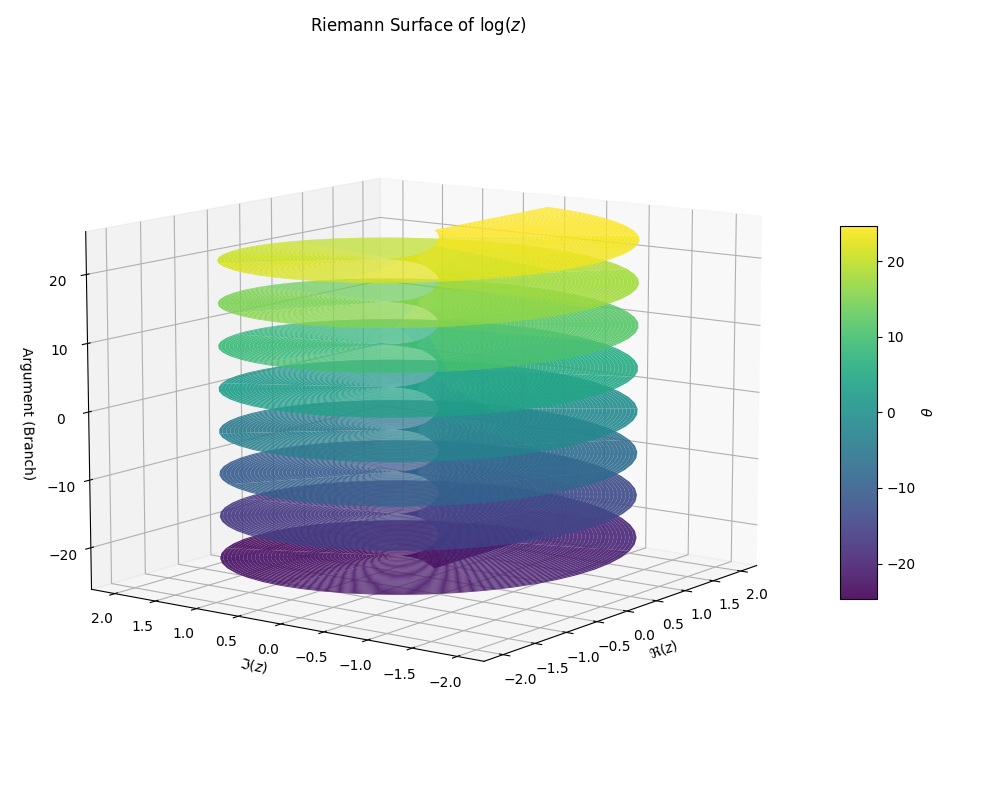
\includegraphics[width=0.85\textwidth]{chapters/chp7_pics/riemann_log.png}
\caption{\textit{The Riemann surface of $\Log(z)$, a helical structure where each sheet represents a branch of $\ln(z)$ for $k \in \mathbb{Z}$, connected along the branch cut at the negative real axis. As $z$ circles the origin, the imaginary part ascends or descends through layers, with $\Log(z)$ as the principal sheet ($-\pi < \Arg(z) \leq \pi$).}}
\label{fig:log-riemann-surface}
\end{figure}

\exampleline
\begin{example}
Compute all values of $\ln(i)$ and the principal value on the Riemann surface.

\begin{solution}
Write $i = e^{i\pi/2}$:
\[
\ln(i) = \ln 1 + i \left( \frac{\pi}{2} + 2\pi k \right) = i \frac{\pi}{2} (1 + 4k), \quad k \in \mathbb{Z},
\]
giving values like $i\pi/2$, $i 5\pi/2$, $i (-\pi/2)$, each on a distinct sheet of the Riemann surface. The principal branch ($-\pi < \Arg(z) \leq \pi$) selects:
\[
\Log(i) = i \frac{\pi}{2},
\]
since $\pi/2$ fits within $(-\pi, \pi]$, anchoring this value to the base sheet.
\end{solution}
\end{example}
\exampleline

\noindent The logarithm’s layered nature, beautifully captured by its Riemann surface, primes us for the next subsection on branch cuts, where we’ll slice through this helical expanse to navigate its many dimensions.

\subsection*{Multiple-Valued Functions and Branch Cuts} \index{Branch Cuts}

\noindent The complex logarithm’s multi-valued nature, stacking outputs like $\ln(-1) = i\pi (1 + 2k)$, hints at a broader phenomenon in $\mathbb{C}$: many functions assign multiple values to a single input. Take the square root: for $z = 4$, $w = 2$ and $w = -2$ both satisfy $w^2 = 4$, doubling the real case. For $z = r e^{i\theta}$, $z^{1/2} = \sqrt{r} e^{i\theta/2}$ or $\sqrt{r} e^{i(\theta/2 + \pi)}$, a pair tied to $e^{i\pi} = -1$. Similarly, $z^{1/n}$ yields $n$ roots, $r^{1/n} e^{i(\theta + 2\pi k)/n}$, $k = 0, 1, \ldots, n-1$, cycling around the origin. \\

\noindent To pin these down, we use \textbf{branch cuts}—lines where we restrict the function to a single \textbf{branch}. For $\ln(z)$, the negative real axis cut gives $\Log(z) = \ln|z| + i \Arg(z)$, $\Arg(z) \in (-\pi, \pi]$. Power functions like $z^{1/3}$ often adopt the same cut, selecting one of three roots. Inverse trigonometric functions, say $\arcsin(z)$, cut from $-\infty$ to $-1$ and $1$ to $\infty$, picking a principal path from infinite possibilities. These cuts, arbitrary yet purposeful, echo the Riemann surface’s layers, slicing a single sheet from the spiral stack. \\

\exampleline
\begin{example}
Find the principal value of $(-8)^{1/3}$, cut along the negative real axis, $\Arg(z) \in (-\pi, \pi]$.

\begin{solution}
Write $-8 = 8 e^{i\pi}$: $(-8)^{1/3} = 8^{1/3} e^{i(\pi + 2\pi k)/3} = 2 e^{i(\pi/3 + 2\pi k/3)}$. For $k = 0, 1, 2$:
\begin{itemize}
\item $k = 0$: $2 e^{i\pi/3} = 1 + i\sqrt{3}$ ($\Arg = \pi/3$),
\item $k = 1$: $2 e^{i\pi} = -2$ ($\Arg = \pi$),
\item $k = 2$: $2 e^{i 5\pi/3} = 1 - i\sqrt{3}$ ($\Arg = -\pi/3$).
All fit $(-\pi, \pi]$, but $k = 0$ is typically principal: $1 + i\sqrt{3}$.
\end{itemize}
\end{solution}
\end{example}
\exampleline

\noindent Branch cuts thus refine multi-valued functions into single-valued tools, their placement shaping our journey through $\mathbb{C}$’s layered expanse.

\subsection*{Computer-Aided Visualization} \index{Complex Visualization Software}

\noindent As we’ve journeyed through the complex plane, from polynomials to logarithms, static sketches have hinted at the richness of these functions. Yet, in an era of digital prowess, software unfurls a new dimension of exploration, breathing life into complex mappings with tools that twist, spin, and zoom at our command. These programs don’t merely draw—they invite us to interact with the mathematics, revealing dynamics that paper alone can’t capture. A direct plot of a complex function, mapping one two-dimensional plane to another, demands four dimensions—a feat beyond a simple page—but computational tools rise to the challenge with elegant solutions like domain coloring. \\

\noindent Domain coloring paints the complex plane with hues and shades to unveil a function’s hidden dance, assigning colors to the range based on its properties. We let \textbf{hue} reflect the argument of $f(z)$, the angle it makes in the plane—picture a color wheel where red marks 0, yellow $\pi/2$, green $\pi$, cycling through the spectrum over $2\pi$—while \textbf{brightness} mirrors the magnitude $|f(z)|$, bright where it soars, dark where it dips. What emerges is a vivid tapestry: \textbf{zeros} appear as dark points, colors converging since $|f(z)|$ vanishes; \textbf{poles} blaze bright, hues spiraling tightly; \textbf{branch cuts} slice as sharp discontinuities—think of $\ln(z)$’s jump from $\pi$ to $-\pi$—and \textbf{periodicity} unfurls in repeating bands. Consider $f(z) = z^2$: software reveals its zero at the origin as a dark center, with hues doubling around it, a visual echo of $\arg(z^2) = 2\arg(z)$. \\

\begin{figure}[H]
\centering
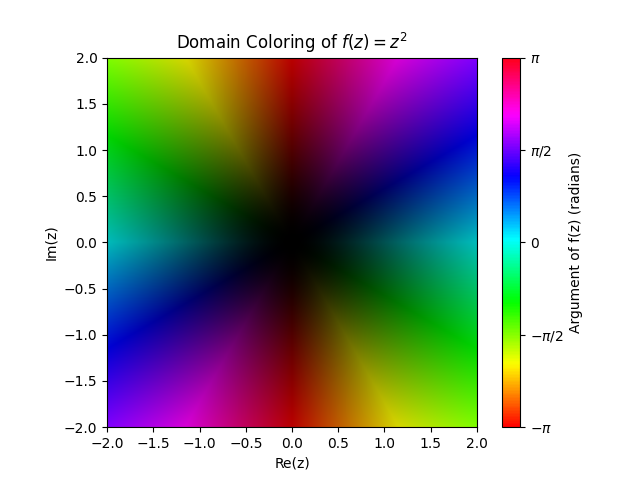
\includegraphics[width=0.8\textwidth]{chapters/chp7_pics/domain_coloring.png}
\caption{\textit{Domain coloring of $f(z) = z^2$, where hue encodes the argument of $f(z)$, ranging from $-\pi$ to $\pi$ to span all directions in the complex plane once, and brightness reflects the magnitude $|f(z)|$ on a logarithmic scale. The doubled cycling of hues around the dark center reveals the angle-doubling property, $\arg(z^2) = 2\arg(z)$, a hallmark of this quadratic mapping.}}
\label{fig:domain-coloring-z2}
\end{figure}

%\noindent You can use this code to provide a domain coloring in Python. \\


\vspace{1.3em} \index{Python}


\begin{lstlisting}[language=Python]
import numpy as np
import matplotlib.pyplot as plt
from matplotlib.colors import hsv_to_rgb
from matplotlib.cm import ScalarMappable

# Define the complex function f(z) = z^2
f = lambda z: z**2

# Set up the grid in the complex plane
x = np.linspace(-2, 2, 400)
y = np.linspace(-2, 2, 400)
X, Y = np.meshgrid(x, y)
Z = X + 1j * Y

# Compute f(z)
W = f(Z)

# Calculate magnitude and argument
magnitude = np.abs(W)
argument = np.angle(W)

# Normalize magnitude for brightness (log scale for better contrast)
magnitude = np.log1p(magnitude)
magnitude = (magnitude - np.min(magnitude)) / (np.max(magnitude) - np.min(magnitude))

# Create HSV image: hue from argument, full saturation, value from magnitude
h = (argument + np.pi) / (2 * np.pi)  # Hue: 0 to 1
s = np.ones_like(h)                   # Saturation: full
v = magnitude                         # Value: brightness
hsv = np.dstack((h, s, v))

# Convert HSV to RGB for plotting
rgb = hsv_to_rgb(hsv)

# Generate the plot
plt.imshow(rgb, extent=(-2, 2, -2, 2), origin='lower')
plt.title(r'Domain Coloring of $f(z) = z^2$')
plt.xlabel('Re(z)')
plt.ylabel('Im(z)')

# Add colorbar for argument
sm = ScalarMappable(cmap='hsv', norm=plt.Normalize(-np.pi, np.pi))
sm.set_array([])  # Required for colorbar to work with ScalarMappable
cbar = plt.colorbar(sm, label='Argument of f(z) (radians)')
cbar.set_ticks([-np.pi, -np.pi/2, 0, np.pi/2, np.pi])
cbar.set_ticklabels([r'$-\pi$', r'$-\pi/2$', r'$0$', r'$\pi/2$', r'$\pi$'])

plt.show()

\end{lstlisting}
\vspace{1.1cm}

\noindent Beyond domain coloring, software offers more wonders: \textbf{interactive plots} let you click a domain point and see its range image, or drag to trace preimages; \textbf{real-time parameter tweaks} shift $f(z) = z^2 + c$ instantly; \textbf{animations} layer transformations like $e^z$ atop $z^2$; and \textbf{surface plots of $|f(z)|$} offer a topographic view of magnitude. These tools sharpen our grasp of \textbf{geometric effects}—addition nudges, multiplication rotates, as with $i z$ at 90 degrees—while zooming near \textbf{singular points} reveals poles flaring or essential singularities writhing. For \textbf{multi-valued functions}, software peels apart branches, stacking $\ln(z)$’s layers, and previews \textbf{conformal mappings}’ angle preservation, as grids bend yet hold shape. \\

\noindent Take $f(z) = e^z$: software maps a grid—horizontal lines to rays, verticals to circles—letting you tilt the view or animate $z$’s path, the output spiraling in rhythm. This builds on the static depiction in Figure \ref{fig:exp-mapping}, amplifying what such figures suggest and opening a window into the function’s soul. \\

\noindent Software also lifts us into three dimensions, offering vivid perspectives on complex functions beyond the flat plane. One approach plots the \textbf{magnitude $|f(z)|$} as a surface over the domain, with height revealing growth—zeros dip to the plane, poles spike skyward, and the function’s scale unfurls in a topographic sweep. For $f(z) = z^2$, this surface rises parabolically from its zero at the origin, a 3D testament to its quadratic stretch across the plane.

\begin{figure}[h]
\centering
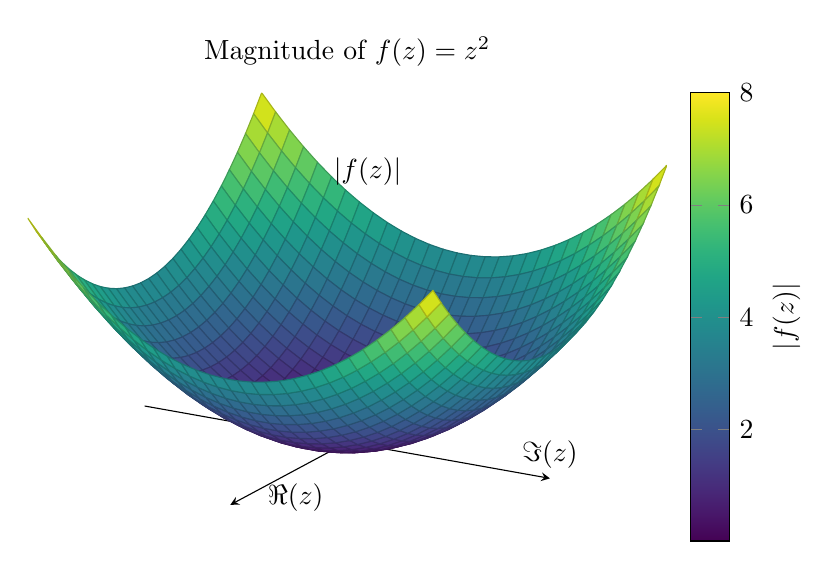
\begin{tikzpicture}
\begin{axis}[
    width=0.8\textwidth,
    height=0.6\textwidth,
    axis lines=center,
    title={Magnitude of $f(z) = z^2$},
    view={120}{30},
    colormap/viridis,
    colorbar,
    colorbar style={ylabel=$|f(z)|$},
    xtick=\empty,
    ytick=\empty,
    ztick=\empty,
]
\addplot3 [
    surf,
    domain=-2:2,
    y domain=-2:2,
    samples=30,
] {x^2 + y^2};

% Add movable labels
\node at (axis cs:1.7,0.1,0) [anchor=west] {$\Re(z)$};
\node at (axis cs:0,2,0) [anchor=south] {$\Im(z)$};
\node at (axis cs:0,0.2,8) [anchor=south] {$|f(z)|$};
\end{axis}
\end{tikzpicture}
\caption{Surface plot of $|f(z)| = |z^2|$ over the complex plane, with height showing magnitude rising quadratically from the zero at the origin.}
\label{fig:magnitude-z2}
\end{figure}

\noindent Alternatively, software can surface the \textbf{real or imaginary parts}, plotting $u(x, y)$ or $v(x, y)$ to trace their undulations over the complex plane. Take $f(z) = e^z$: its real part $e^x \cos y$ blends exponential growth along the real axis with cosine waves along the imaginary, a 3D ripple that echoes its oscillatory nature. Then there’s the \textbf{Riemann surface}, stacking multi-valued outputs like $\ln(z)$’s spiral sheets, as seen in Figure \ref{fig:log-riemann-surface}, where branches connect across cuts in a helical dance. These 3D views—crafted by tools like Python or Mathematica—bring the invisible into focus, marrying computation with intuition.

\begin{figure}[h]
\centering
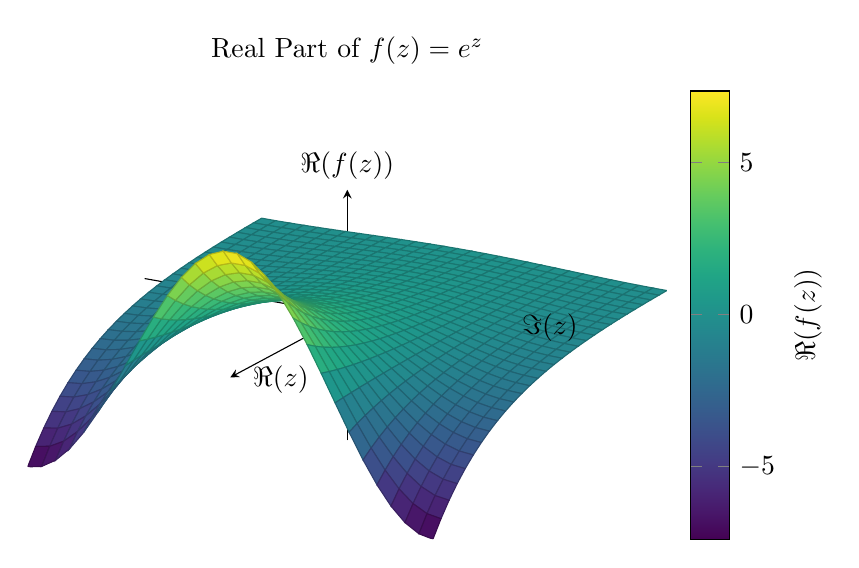
\begin{tikzpicture}
\begin{axis}[
    width=0.8\textwidth,
    height=0.6\textwidth,
    axis lines=center,
    title={Real Part of $f(z) = e^z$},
    view={120}{30},
    colormap/viridis,
    colorbar,
    colorbar style={ylabel=$\Re(f(z))$},
    xtick=\empty,  % Remove x-axis ticks
    ytick=\empty,  % Remove y-axis ticks
    ztick=\empty,  % Remove z-axis ticks
]
\addplot3 [
    surf,
    domain=-2:2,
    y domain=-3.1416:3.1416,
    samples=30,
] {exp(x)*cos(deg(y))};

% Movable labels
\node at (axis cs:2,0.2,0) [anchor=west] {$\Re(z)$};         % Label for Re(z)
\node at (axis cs:0,3.1416,0) [anchor=south] {$\Im(z)$};   % Label for Im(z)
\node at (axis cs:0,0,7.4) [anchor=south] {$\Re(f(z))$};   % Label for Re(f(z))
\end{axis}
\end{tikzpicture}
\caption{Surface plot of the real part of $f(z) = e^z$, where $u(x, y) = e^x \cos y$ blends exponential growth along the real axis with cosine oscillations along the imaginary.}
\label{fig:real-exp}
\end{figure}

\noindent These visualizations, from domain coloring to 3D surfaces, are ingenious compromises. A complex function \( f: \mathbb{C} \to \mathbb{C} \) demands four dimensions—two for the input \( z \), two for the output \( f(z) \)—but our tools are bound to three or two. Domain coloring squeezes both magnitude and argument into a 2D image via color, while surface plots of \( |f(z)| \), \( \Re(f(z)) \), or \( \Im(f(z)) \) reduce the output to one real number, plotted over the complex plane in 3D. Riemann surfaces stack multi-valued outputs, hinting at the function's layers. Each method sacrifices a dimension to make the invisible visible, offering a glimpse into the function's soul at the cost of completeness.

\newpage
\lecture{Basic Limits in Complex Analysis} \index{Limits}

\noindent In Chapter 3, Lecture 2, we developed the epsilon–delta definition of limits for functions in \(\mathbb{R}^n\). When we move into complex analysis, the formal definition remains identical—using the modulus \(|z-z_0|\) as our measure of distance—but the two-dimensional nature of \(\mathbb{C}\) and its algebraic structure open up additional techniques for evaluating limits. In this lecture, we expand on the basics of complex limits, highlight methods unique to the complex setting, and explain in detail how to handle expressions involving complex conjugates.

\subsection*{Basic Definition and Similarities}

\noindent Let \(f: D \to \mathbb{C}\) be a function defined on a domain \(D \subseteq \mathbb{C}\), and let \(z_0\) be a limit point of \(D\). We say that 
\[
\lim_{z \to z_0} f(z) = L
\]
if for every \(\epsilon > 0\) there exists a \(\delta > 0\) such that for all \(z \in D\) with \(0 < |z - z_0| < \delta\) we have
\[
|f(z) - L| < \epsilon.
\]
This is exactly the epsilon–delta definition used in \(\mathbb{R}^n\), with the key difference that here distance is measured by the modulus \(|z-z_0|\). Because \(\mathbb{C}\) is essentially \(\mathbb{R}^2\), many aspects of higher-dimensional limits carry over directly. However, the two-dimensional nature of \(\mathbb{C}\) introduces an important nuance: there are infinitely many directions from which \(z\) can approach \(z_0\). \\

\noindent In \(\mathbb{R}^n\), we typically consider sequences or paths converging to a point and verify that the limit is independent of the chosen path. In \(\mathbb{C}\), this requirement is even more critical. For the limit \(L\) to exist, the condition \(|f(z) - L| < \epsilon\) must hold regardless of the angle or path along which \(z\) approaches \(z_0\). This path-independence guarantees the uniqueness of the limit and is automatically satisfied in one-dimensional real analysis, but must be explicitly checked in the complex setting. Thus, while the definition is formally the same as in \(\mathbb{R}^n\), the complex case forces us to account for a richer set of approaches to a limit point.



\begin{figure}[H]
\centering
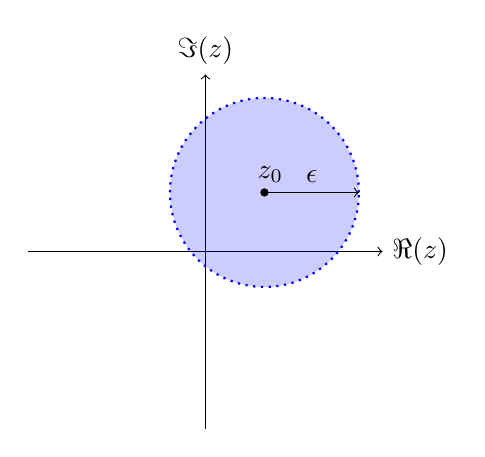
\begin{tikzpicture}[scale=1.5]
  % Draw axes
  \draw[->] (-1.5,0) -- (1.5,0) node[right] {$\Re(z)$};
  \draw[->] (0,-1.5) -- (0,1.5) node[above] {$\Im(z)$};

  % Draw open disk (dotted border)
  \fill[blue, opacity=0.2] (0.5,0.5) circle (0.8);
  \draw[blue, thick, dotted] (0.5,0.5) circle (0.8);

  % Mark z_0
  \fill (0.5,0.5) circle (1pt);
  \node at (0.55,0.65) {$z_0$};  % Move this coordinate to adjust label position

  % Radius arrow
  \draw[->] (0.5,0.5) -- (1.3,0.5) node[midway, above] {$\epsilon$};
\end{tikzpicture}
\caption{An open disk \(D(z_0, \epsilon)\) centered at \(z_0\) with radius \(\epsilon\) in the complex plane.}
\label{fig:open-disk}
\end{figure}


\subsection*{New Techniques in Evaluating Complex Limits}

\noindent Although the basic epsilon–delta definition remains unchanged, several additional techniques are especially useful in complex analysis:

\begin{itemize}
    \item \textbf{Use of Polar Form:} Expressing a complex number \(z\) in polar coordinates as
    \[
    z = re^{i\theta},
    \]
    where \(r = |z|\) and \(\theta = \arg(z)\), can simplify the evaluation of limits. In many cases, limits reduce to a function of \(r\) (the distance from the origin) and \(\theta\) (the angle of approach). This method also helps us check if the limit is path-independent; if the limit depends on \(\theta\), it does not exist.
    
    \item \textbf{Series Expansion:} Similar to real analysis, Taylor series expansions for functions such as \(\sin(z)\), \(\cos(z)\), or \(e^z\) allow us to approximate and evaluate limits. For example, expanding \(\sin(z)\) as
    \[
    \sin(z) = z - \frac{z^3}{3!} + \frac{z^5}{5!} - \cdots,
    \]
    simplifies the evaluation of \(\frac{\sin(z)}{z}\) as \(z\) approaches 0.
    
    \item \textbf{Handling Complex Conjugates:} Complex conjugates play a special role in \(\mathbb{C}\). If \(z = re^{i\theta}\), then the conjugate is given by
    \[
    \overline{z} = re^{-i\theta}.
    \]
    This relationship is extremely useful in simplifying expressions where both \(z\) and \(\overline{z}\) appear. For example, note that \(|z|^2 = z\overline{z}\) and that ratios like \(\frac{\overline{z}}{z}\) can be expressed in terms of the argument \(\theta\), as we will see.
    
    \item \textbf{Modulus and Argument Techniques:} By decomposing a complex number into its modulus and argument, we can often determine if a limit is well-defined. If the limit expression depends on the angle \(\theta\) (i.e., the direction of approach), then the limit might not exist. This method is particularly useful when dealing with functions that do not behave uniformly in every direction.
\end{itemize}

\noindent A common scenario in complex limits is the appearance of the complex conjugate. Consider the ratio:
\[
\frac{\overline{z}}{z}.
\]
Express \(z\) in polar form as \(z = re^{i\theta}\). Then the conjugate is \(\overline{z} = re^{-i\theta}\), and the ratio simplifies to
\[
\frac{\overline{z}}{z} = \frac{re^{-i\theta}}{re^{i\theta}} = e^{-2i\theta}.
\]
Here, the modulus of the expression is always 1, but its value depends entirely on the angle \(\theta\). As \(z \to 0\), although \(r\) tends to 0, the value of \(\theta\) may vary depending on the path taken toward the origin. For example:
\begin{itemize}
    \item Along the positive real axis (\(\theta = 0\)), \(e^{-2i\theta} = 1\).
    \item Along the positive imaginary axis (\(\theta = \pi/2\)), \(e^{-2i\theta} = e^{-i\pi} = -1\).
\end{itemize}
Since the limit depends on the direction of approach, the limit of \(\frac{\overline{z}}{z}\) as \(z \to 0\) does not exist.

\subsection*{Properties of Limits in \(\mathbb{C}\)}

\noindent The algebraic properties of limits that you are familiar with from real analysis extend naturally to complex functions. Suppose that 
\[
\lim_{z \to z_0} f(z) = L \quad \text{and} \quad \lim_{z \to z_0} g(z) = M.
\]
Then the following properties hold:
\begin{itemize}
  \item \(\displaystyle \lim_{z \to z_0} \bigl(f(z) + g(z)\bigr) = L + M\).
  \item \(\displaystyle \lim_{z \to z_0} \bigl(f(z) \cdot g(z)\bigr) = L \cdot M\).
  \item For any constant \(c \in \mathbb{C}\), \(\displaystyle \lim_{z \to z_0} c\,f(z) = c\,L\).
  \item If \(M \neq 0\), \(\displaystyle \lim_{z \to z_0} \frac{f(z)}{g(z)} = \frac{L}{M}\).
\end{itemize}
These properties rely on the fact that the modulus \(|\cdot|\) in \(\mathbb{C}\) obeys the triangle inequality and product rule, much like the Euclidean norm in \(\mathbb{R}^2\). The proofs of these properties follow along the same lines as in Chapter 3, Lecture 2, and serve as a useful bridge between real and complex analysis.

\exampleline
\begin{example}
Evaluate the following limits:
\begin{enumerate}
    \item \( \displaystyle \lim_{z \to 0} z^2 \)
    \item \( \displaystyle \lim_{z \to 0} \frac{\sin(z)}{z} \)
    \item \( \displaystyle \lim_{z \to 0} \frac{|z|^2}{z} \)
    \item \( \displaystyle \lim_{z \to 0} \frac{\overline{z}}{z} \)
\end{enumerate}

\begin{solution}
\begin{enumerate}
    \item \textbf{Limit of \(z^2\):}  
    Since \(z^2\) is a polynomial, it is continuous everywhere in \(\mathbb{C}\). Therefore, by direct substitution:
    \[
    \lim_{z \to 0} z^2 = 0^2 = 0.
    \]

    \item \textbf{Limit of \(\frac{\sin(z)}{z}\):}  
    The Taylor series for \(\sin(z)\) is:
    \[
    \sin(z) = z - \frac{z^3}{3!} + \frac{z^5}{5!} - \cdots.
    \]
    Dividing by \(z\) yields:
    \[
    \frac{\sin(z)}{z} = 1 - \frac{z^2}{3!} + \frac{z^4}{5!} - \cdots.
    \]
    As \(z \to 0\), all terms involving \(z\) vanish, hence:
    \[
    \lim_{z \to 0} \frac{\sin(z)}{z} = 1.
    \]

    \item \textbf{Limit of \(\frac{|z|^2}{z}\):}  
    Recall that \(|z|^2 = z \overline{z}\). Thus, for \(z \neq 0\):
    \[
    \frac{|z|^2}{z} = \frac{z\overline{z}}{z} = \overline{z}.
    \]
    As \(z \to 0\), \(\overline{z} \to 0\) (since complex conjugation is continuous), so:
    \[
    \lim_{z \to 0} \frac{|z|^2}{z} = 0.
    \]

    \item \textbf{Limit of \(\frac{\overline{z}}{z}\):}  
    Write \(z = re^{i\theta}\) so that \(\overline{z} = re^{-i\theta}\). Then,
    \[
    \frac{\overline{z}}{z} = e^{-2i\theta}.
    \]
    Since this expression depends on the angle \(\theta\) and not on the magnitude \(r\), different paths to 0 (with different \(\theta\)) yield different values. For example:
    \begin{itemize}
        \item If \(z\) approaches 0 along the positive real axis (\(\theta=0\)), then \(\frac{\overline{z}}{z} = 1\).
        \item If \(z\) approaches 0 along the positive imaginary axis (\(\theta=\pi/2\)), then \(\frac{\overline{z}}{z} = e^{-i\pi} = -1\).
    \end{itemize}
    Therefore, the limit does not exist.
\end{enumerate}
\end{solution}
\end{example}
\exampleline

\noindent In summary, while the fundamental definition of limits in \(\mathbb{C}\) mirrors that in \(\mathbb{R}^n\), the additional structure of complex numbers allows us to employ techniques such as polar representation and series expansions. These methods, along with careful treatment of expressions involving complex conjugates, are essential tools in evaluating complex limits and in detecting path-dependent behavior.


\subsection*{Continuity and Topological Foundations in \(\mathbb{C}\)}

\noindent In complex analysis, the notion of continuity is defined in exactly the same way as in real analysis using the epsilon–delta formulation. However, the two-dimensional structure of \(\mathbb{C}\) and its rich topology provide additional tools and perspectives that are crucial for a deeper understanding of limits and continuity. In this section, we discuss these foundational ideas and illustrate their usefulness with detailed examples.

\subsubsection*{Continuity in \(\mathbb{C}\)}

\noindent Let \(f: D \to \mathbb{C}\) be a function on a domain \(D \subseteq \mathbb{C}\) and let \(z_0\) be a limit point of \(D\). We say that 
\[
\lim_{z \to z_0} f(z) = L
\]
if for every \(\epsilon > 0\) there exists a \(\delta > 0\) such that whenever \(z \in D\) with \(0 < |z-z_0| < \delta\) it follows that
\[
|f(z) - L| < \epsilon.
\]
This definition uses the modulus \(|z-z_0|\) as the distance measure, leveraging the fact that \(\mathbb{C}\) is isometric to \(\mathbb{R}^2\).

An equivalent formulation employs open sets: \(f\) is continuous at \(z_0\) if for every open neighborhood \(V\) of \(f(z_0)\) there is an open neighborhood \(U\) of \(z_0\) such that
\[
f(U) \subseteq V.
\]
In \(\mathbb{C}\), open neighborhoods are typically open disks of the form
\[
D(z_0, \epsilon) = \{ z \in \mathbb{C} : |z-z_0| < \epsilon \}.
\]
\exampleline
\begin{example}
Consider the function \(f(z) = |z|^2 = z\overline{z}\). Show that \(f\) is continuous at any \(z_0 \in \mathbb{C}\).
\begin{solution}
Let \(\epsilon > 0\) be given. We wish to find a \(\delta > 0\) such that for all \(z\) with \(|z-z_0| < \delta\),
\[
\bigl||z|^2 - |z_0|^2\bigr| = |z\overline{z} - z_0\overline{z_0}| < \epsilon.
\]
Notice that
\[
|z\overline{z} - z_0\overline{z_0}| = |z(\overline{z}-\overline{z_0}) + \overline{z_0}(z-z_0)| \leq |z||z-z_0| + |z_0||z-z_0|.
\]
Since \(|z-z_0|<1\) implies \(|z| \le |z_0| + 1\), we have
\[
|f(z) - f(z_0)| < \bigl((|z_0|+1) + |z_0|\bigr)|z-z_0| = (1+2|z_0|)|z-z_0|.
\]
Thus, choosing
\[
\delta = \min\left\{1,\,\frac{\epsilon}{1+2|z_0|}\right\},
\]
ensures that \(|f(z)-f(z_0)| < \epsilon\) whenever \(|z-z_0| < \delta\). Hence, \(f\) is continuous at \(z_0\).
\end{solution}
\end{example}
\exampleline
\subsubsection*{Topological Properties of \(\mathbb{C}\) and Their Usefulness}

The rich topological structure of \(\mathbb{C}\) – inherited from its homeomorphism with \(\mathbb{R}^2\) – provides us with powerful tools such as open sets, connectedness, and compactness, which are essential for rigorously understanding limits and continuity. In the following sections, we will develop these technical foundations further to deepen our understanding of continuity in complex analysis.\\

\noindent \textbf{Open Sets:} \noindent One of the cornerstones of topology—and by extension, of continuity and limit theory—is the concept of an open set. In Chapter 3, Lecture 2, we covered the basics of open sets in \(\mathbb{R}^n\). Since \(\mathbb{C}\) is very similar to \(\mathbb{R}^2\), these ideas translate directly to the complex plane with an added geometric elegance.\\

\noindent In \(\mathbb{C}\), every open set can be expressed as a union of open disks. An open disk centered at \(z_0\) with radius \(\epsilon\) is defined by
\[
D(z_0, \epsilon) = \{ z \in \mathbb{C} : |z - z_0| < \epsilon \}.
\]
This disk is the basic building block or ``neighborhood" of \(z_0\) in the complex plane. It provides a precise way to describe what it means for points to be ``close" to \(z_0\) using the modulus as a distance measure. \\

\noindent The usefulness of open disks becomes evident when we prove local properties like continuity. Specifically, to show that a function \(f\) is continuous at a point \(z_0\), one must show that for every open disk \(D(f(z_0), \eta)\) around \(f(z_0)\) in the codomain, there exists an open disk \(D(z_0, \epsilon)\) around \(z_0\) in the domain such that
\[
f\bigl(D(z_0, \epsilon)\bigr) \subseteq D(f(z_0), \eta).
\]
This topological formulation is entirely equivalent to the epsilon–delta definition but emphasizes the spatial, geometric intuition behind continuity.

\exampleline
\begin{example}
Consider again \(f(z)=z^2\). Demonstrate that for any open disk \(D(z_0, \epsilon)\) centered at \(z_0\), there exists an open disk \(D(f(z_0), \eta)\) such that
\[
f\bigl(D(z_0, \epsilon)\bigr) \subseteq D(f(z_0), \eta).
\]
\begin{solution}
Since \(f(z)=z^2\) is continuous, for any \(\eta > 0\) there exists \(\delta > 0\) so that if \(|z-z_0| < \delta\) then
\[
|z^2-z_0^2| = |z-z_0||z+z_0| < \eta.
\]
By choosing \(\delta\) sufficiently small (ensuring, for example, that \(|z-z_0| < 1\) so that \(|z+z_0|\) is bounded), we guarantee that the entire disk \(D(z_0, \delta)\) is mapped inside \(D(z_0^2, \eta)\). 
\end{solution}
\end{example}
\exampleline

\noindent \textbf{Connectedness:}  The complex plane \(\mathbb{C}\) is a prime example of a connected space—it is not only connected but also path-connected. This means that for any two points \(z_1, z_2 \in \mathbb{C}\), there exists a continuous path \(\gamma: [0,1] \to \mathbb{C}\) such that \(\gamma(0)=z_1\) and \(\gamma(1)=z_2\). In practical terms, this property implies that the complex plane cannot be split into two disjoint nonempty open subsets.  \\

\noindent Connectedness has profound implications in analysis. One of the key theorems states that if a function \(f: D \to \mathbb{C}\) is continuous on a connected domain \(D\), then the image \(f(D)\) is also connected. This result is critical because it ensures that continuous functions cannot “break apart” the domain into separate pieces. As a consequence, if a continuous function takes two distinct values on a connected set, it must take every value in between (this is an extension of the intermediate value property to connected sets in \(\mathbb{C}\)). \\

\noindent The equivalence of connectedness and path-connectedness in \(\mathbb{C}\) (a feature of all metric spaces like \(\mathbb{R}^2\)) further simplifies many arguments. When dealing with limits and continuity, knowing that any two points are joined by some continuous path allows us to analyze function behavior along various paths and conclude that the limit (or image) must be the same regardless of the chosen path.


\begin{example}
Let \(f(z) = e^z\). Prove that \(e^{\mathbb{C}}\) is connected.
\begin{solution}
The function \(f(z)=e^z\) is continuous and maps \(\mathbb{C}\) onto \(\mathbb{C}\setminus\{0\}\). Since \(\mathbb{C}\) is path-connected, any continuous image of \(\mathbb{C}\) must be connected. Therefore, \(e^{\mathbb{C}} = \mathbb{C}\setminus\{0\}\) is connected.
\end{solution}
\end{example}

\begin{figure}[H]
\centering
\begin{tikzpicture}[scale=1.5]
  \draw[->, thick] (-0.5,0) -- (2,0) node[right] {$\Re(z)$};
  \draw[->, thick] (0,-0.5) -- (0,2) node[above] {$\Im(z)$};
  \fill (0.5,0.5) circle (2pt) node[below left] {\(z_1\)};
  \fill (1.5,1.2) circle (2pt) node[above right] {\(z_2\)};
  \draw[red, thick, ->] (0.5,0.5) .. controls (1,1.5) and (1.2,0.2) .. (1.5,1.2);
\end{tikzpicture}
\caption{Any two points in \(\mathbb{C}\) can be connected by a continuous path.}
\label{fig:connected-path}
\end{figure}

\noindent \textbf{Compactness:}  In the setting of \(\mathbb{C}\) (which, as we know, is essentially \(\mathbb{R}^2\)), a set is called compact if it is both closed and bounded. Here, a set is \emph{closed} if it contains all its boundary points, and it is \emph{bounded} if it can be entirely contained within a disk of some finite radius. This result is known as the \textbf{Heine–Borel theorem}. \index{Heine-Borel Theorem}Compact sets are very useful in analysis because any continuous function defined on a compact set is guaranteed to reach both a maximum and a minimum value—a fact learned earlier as the Extreme Value Theorem. This property helps ensure that functions behave in a controlled manner, which is critical when dealing with limits.
\exampleline
\begin{example}
Let 
\[
A = \{ z \in \mathbb{C} : 1 \leq |z| \leq 2 \}
\]
be the closed annulus in \(\mathbb{C}\). First, show that \(A\) is compact. Then, consider the function 
\[
f(z) = z^2.
\]
Show that \(f\) is continuous on \(A\) and deduce that \(f(A)\) is compact. Finally, determine the range of \(|f(z)|\) on \(A\) and verify that \(f\) attains its maximum and minimum values.

\begin{solution}
\begin{enumerate}
\item \textbf{Prove \(A\) is Compact.}
The set \(A\) is defined by the condition \(1 \leq |z| \leq 2\). It is bounded because every \(z \in A\) satisfies \(|z| \leq 2\), and it is closed because it includes all points on its boundary (those with \(|z|=1\) and \(|z|=2\)). By the Heine–Borel theorem, every closed and bounded subset of \(\mathbb{R}^2\) is compact. Since \(\mathbb{C}\) is homeomorphic to \(\mathbb{R}^2\), \(A\) is compact.

\item \textbf{Show \(f(z) = z^2\) is Continuous on \(A\) and \(f(A)\) is Compact.}
Since \(f(z)=z^2\) is a polynomial, it is continuous on the entire complex plane, and in particular on the compact set \(A\). The continuous image of a compact set is compact, so \(f(A)\) is compact.

\item \textbf{Determine the Range of \(|f(z)|\) on \(A\).}
Notice that for any \(z \in \mathbb{C}\),
\[
|f(z)| = |z^2| = |z|^2.
\]
Since \(z \in A\) satisfies \(1 \leq |z| \leq 2\), we have:
\[
1^2 \leq |z|^2 \leq 2^2 \quad \Longrightarrow \quad 1 \leq |f(z)| \leq 4.
\]
Thus, the minimum modulus of \(f(z)\) on \(A\) is 1, and the maximum modulus is 4. These extreme values are attained when \(|z| = 1\) (yielding \(|f(z)| = 1\)) and when \(|z| = 2\) (yielding \(|f(z)| = 4\)), respectively.

\item \textbf{Conclusion:}
We have shown that the closed annulus 
\[
A = \{ z \in \mathbb{C} : 1 \leq |z| \leq 2 \}
\]
is compact. The function \(f(z) = z^2\) is continuous on \(A\), so its image \(f(A)\) is also compact. Moreover, since \(|f(z)| = |z|^2\), the range of \(|f(z)|\) on \(A\) is the interval \([1,4]\), meaning that \(f\) attains a minimum modulus of 1 and a maximum modulus of 4 on \(A\).

\end{enumerate}
\end{solution}
\end{example}
\exampleline

\noindent \textbf{Extended Complex Plane:} To study limits that involve behavior ``at infinity,” it is useful to introduce the extended complex plane, denoted
\[
\hat{\mathbb{C}} = \mathbb{C} \cup \{\infty\}.
\]
This construction ``adds” a single point at infinity to \(\mathbb{C}\), thereby compactifying the plane and making it homeomorphic to the Riemann sphere. In other words, by including \(\infty\), we transform \(\mathbb{C}\) from an unbounded space into a compact space, which has many desirable properties in analysis. \\

\noindent One major advantage of working in the extended complex plane is that it allows us to handle limits at infinity in a manner analogous to limits at finite points. Specifically, we define
\[
\lim_{z \to \infty} f(z) = L
\]
if, for every \(\epsilon > 0\), there exists an \(R > 0\) such that whenever \(|z| > R\) (that is, \(z\) lies outside a disk of radius \(R\)), it follows that
\[
|f(z) - L| < \epsilon.
\]
\noindent This definition mirrors the standard epsilon–delta definition of a limit, but with the roles reversed: instead of \(z\) approaching a specific finite point, we require the values of \(f(z)\) to approach \(L\) as \(z\) ``escapes” to infinity. \\

\noindent The compactification of \(\mathbb{C}\) via the addition of \(\infty\) is not merely a technical trick—it has significant consequences. For example, many theorems that hold on compact sets (such as the Extreme Value Theorem) can now be extended to functions defined on \(\hat{\mathbb{C}}\). Moreover, considering limits at infinity in this framework unifies our approach to finite and infinite limits. \\

\noindent To visualize the extended complex plane, one often uses the Riemann sphere. Imagine the complex plane as the equatorial plane of a sphere. Each point in \(\mathbb{C}\) corresponds to a point on the sphere via stereographic projection, and the ``north pole” of the sphere represents the point at infinity. This geometric picture helps us understand how sequences that ``escape” to infinity in \(\mathbb{C}\) are seen as converging to the north pole on the Riemann sphere.

\begin{figure}[H]
\centering
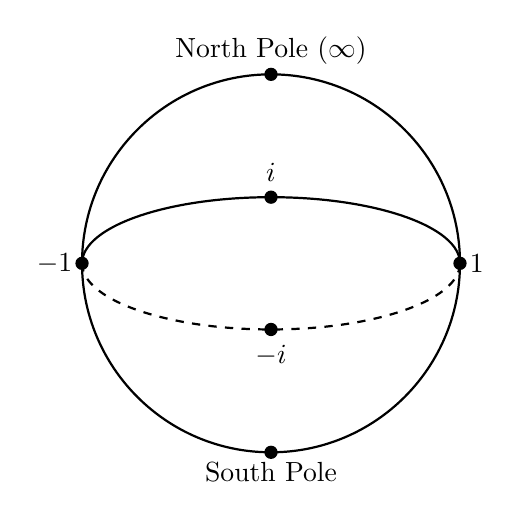
\begin{tikzpicture}[scale=1.2]

  % Draw the outer circle representing the sphere
  \draw[thick] (0,0) circle (2cm);
  
  % Draw the "equator" as a horizontal ellipse
  % Dashed back half from left to right
  \draw[dashed, thick] (-2,0) arc (180:360:2cm and 0.7cm);
  % Solid front half from right to left
  \draw[thick] (2,0) arc (0:180:2cm and 0.7cm);
  
  % Mark the north pole (representing infinity)
  \fill (0,2) circle (2pt) node[above] {North Pole (\(\infty\))};
  
  % Mark the south pole
  \fill (0,-2) circle (2pt) node[below] {South Pole};
  
  % Approximate positions of 1, -1, i, and -i on the equator
  % We'll place them around the circle at cardinal points for illustration.
  
  % Right intersection (approx) for z=1
  \fill (2,0) circle (2pt) node[right] {$1$};
  
  % Left intersection (approx) for z=-1
  \fill (-2,0) circle (2pt) node[left] {$-1$};
  
  % Intersection near the "front" of the equator for z=i (we'll place it above the center)
  % Since this is a 2D projection, let's approximate i at some arc in the top half of the equator
  % We can place it at a param or angle. Let's do something simpler:
  \fill (0,0.7) circle (2pt) node[above=2pt] {$i$};
  
  % Intersection near the "front" of the equator for z=-i (we'll place it below the center)
  \fill (0,-0.7) circle (2pt) node[below=2pt] {$-i$};
  
  % We might optionally label the equator or do more arcs if desired
  
\end{tikzpicture}
\caption{A schematic of the Riemann sphere representing the extended complex plane 
\(\hat{\mathbb{C}} = \mathbb{C} \cup \{\infty\}\). The north pole corresponds to the 
point at infinity, while the equator (solid and dashed) is a cross-sectional view of 
the complex plane. The points \(1\), \(-1\), \(i\), and \(-i\) are placed at approximate 
locations on the equator for illustrative purposes.}
\label{fig:riemann-sphere-labeled}
\end{figure}



\exampleline
\begin{example}
Show that
\[
\lim_{z \to 0} \frac{1}{z} = \infty
\]
in the extended complex plane.
\begin{solution}
For \(z \neq 0\),
\[
\left|\frac{1}{z}\right| = \frac{1}{|z|}.
\]
As \(z \to 0\), \(|z|\) becomes arbitrarily small, and consequently, \(\frac{1}{|z|}\) becomes arbitrarily large. Formally, for any \(M > 0\), if we choose \(\delta = \frac{1}{M}\) then whenever \(0 < |z| < \delta\), we have
\[
\left|\frac{1}{z}\right| > M.
\]
Thus, in \(\hat{\mathbb{C}}\), we write
\[
\lim_{z \to 0} \frac{1}{z} = \infty.
\]
This concept is best visualized via the Riemann sphere, where the point at infinity “completes” the compact space.
\end{solution}
\end{example}
\exampleline

\noindent In summary, the topological properties of \(\mathbb{C}\)—including the structure of open sets, connectedness, and compactness, as well as the notion of the extended complex plane—provide a rigorous framework for understanding limits. These properties are essential not only in establishing basic limit results but also in preparing us for more advanced topics in the theory of generalized change.

\subsubsection*{Sequential Continuity in \(\mathbb{C}\)}

\noindent In addition to the epsilon–delta definition, continuity in the complex plane can also be characterized via sequences. Specifically, a function \(f: D \to \mathbb{C}\) is \textbf{sequentially continuous} at a point \(z_0\) if, for every sequence \(\{z_n\}\) in \(D\) converging to \(z_0\), the sequence \(\{f(z_n)\}\) converges to \(f(z_0)\). This viewpoint can be especially intuitive in \(\mathbb{C}\) because there are infinitely many directions from which a point can approach \(z_0\). By considering \emph{all} sequences that converge to \(z_0\), we ensure that the limit of \(f(z)\) is path-independent. If different sequences converging to \(z_0\) yield different limits for \(\{f(z_n)\}\), then \(f\) cannot be continuous at \(z_0\). This sequential perspective thus confirms that continuity demands uniformity of behavior in every direction in the complex plane.

\exampleline
\begin{example}
Consider the function 
\[
f(z) = \frac{\overline{z}}{z}, \quad z \neq 0.
\]
Express \(z\) in polar form as \(z = re^{i\theta}\), so that \(\overline{z} = re^{-i\theta}\). Then,
\[
f(z) = \frac{re^{-i\theta}}{re^{i\theta}} = e^{-2i\theta}.
\]
Now, observe that if we take different sequences approaching 0 with different fixed angles \(\theta\), the value of \(e^{-2i\theta}\) will vary. For instance:
\begin{itemize}
    \item If \(z\) approaches 0 along the positive real axis (\(\theta = 0\)), then \(f(z) = e^0 = 1\).
    \item If \(z\) approaches 0 along the positive imaginary axis (\(\theta = \pi/2\)), then \(f(z) = e^{-i\pi} = -1\).
\end{itemize}
Because the limit depends on the direction of approach, \(f\) is not sequentially continuous at \(z = 0\).
\begin{solution}
Since different sequences approaching \(0\) yield different limit values, by the sequential criterion, \(f(z) = \frac{\overline{z}}{z}\) does not have a unique limit as \(z \to 0\). Hence, \(f\) is not continuous at 0.
\end{solution}
\end{example}
\exampleline

\noindent In conclusion, the interplay between the topology of \(\mathbb{C}\) and the study of limits is central to complex analysis. By understanding open sets, connectedness, and compactness—and by applying both epsilon–delta and sequential definitions of continuity—we establish a robust framework for analyzing how functions behave in the complex plane. This foundational work is indispensable not only for basic limit proofs but also for the more advanced topics that follow. \\

\noindent In particular, these topological and continuity concepts pave the way for \emph{complex differentiability} (also known as \emph{holomorphy}), where a function has a complex derivative at every point in a domain. Holomorphic functions, in turn, exhibit remarkable properties such as \emph{analyticity}, meaning they can be locally represented by power series and have infinitely many derivatives. These deeper results in complex analysis—such as the Cauchy integral theorems, the Maximum Modulus Principle, and analytic continuation—all rely heavily on the topological underpinnings we have established here.  \\

\noindent Thus, by thoroughly understanding limits and continuity in the context of open sets, connected domains, and compact subsets of \(\mathbb{C}\), we equip ourselves with the essential “toolkit” needed to explore the elegant and far-reaching consequences of holomorphic functions in the broader theory of generalized change. 


\newpage




\newpage

\lecture{Complex Differentiation} \index{Complex Differentiation}

\noindent In calculus and real analysis, the derivative is defined as the limit of the difference quotient—a tool that provides the best linear approximation to a function at a given point. But what does it mean to differentiate a function on the complex plane, where every point has infinitely many directions of approach? The idea is similar: we wish for the limit
\[
f'(z_0)=\lim_{\Delta z \to 0}\frac{f(z_0+\Delta z)-f(z_0)}{\Delta z}
\]
to exist. However, because the complex plane is two-dimensional, this limit must be the same regardless of the path along which \(\Delta z\) (or equivalently, \(z-z_0\)) approaches zero. In other words, \(f'(z_0)\) must be independent of the direction of approach. This extra requirement is what makes complex differentiability a much stronger condition than in the real setting.

\subsection*{Motivation and Definition} \index{Holomorphic Functions}

\noindent Recall that every complex number \(z\) can be expressed as
\[
z = x + iy,
\]
and accordingly a function \(f\) defined on a domain \(D\subset\mathbb{C}\) can be written as
\[
f(z)=u(x,y)+iv(x,y).
\]
We say that \(f\) is \textbf{complex differentiable} (or \textbf{holomorphic}) at a point \(z_0\in D\) if
\[
f'(z_0)=\lim_{\Delta z\to 0}\frac{f(z_0+\Delta z)-f(z_0)}{\Delta z}
\]
exists and is independent of the manner in which \(\Delta z\) approaches 0. This condition ensures that, locally, the function can be well-approximated by the linear map
\[
f(z) \approx f(z_0)+f'(z_0)(z-z_0),
\]
where \(f'(z_0)\) acts as both a scaling factor (its modulus \(|f'(z_0)|\)) and a rotation (its angle \(\arg(f'(z_0))\)). In the one-dimensional real setting the function has only two possible directions (from the left or the right), but in \(\mathbb{C}\) there is a continuum of directions. This stronger requirement forces the real and imaginary parts of \(f\) to satisfy interrelated conditions, later formalized as the Cauchy-Riemann equations. \\

\noindent To illustrate the concept, consider the following simplified diagram. The left side shows an \(\epsilon\)-neighborhood (a circle) in the \(z\)-plane centered at \(z_0\). The requirement is that, no matter which point \(z\) is chosen on this circle, the difference quotient
\[
\frac{f(z)-f(z_0)}{z-z_0} \quad \text{(or equivalently, } \frac{f(z_0+\Delta z)-f(z_0)}{\Delta z}\text{)}
\]
tends to the same complex number \(f'(z_0)\). The right side of the diagram depicts the corresponding linear approximation in the \(w\)-plane.

\begin{figure}[H]
    \centering
    \begin{tikzpicture}[scale=1.2]
        % Define coordinate systems for z-plane
        \draw[->] (-2,0) -- (2,0) node[right] {$\text{Re}(z)$};
        \draw[->] (0,-2.5) -- (0,2.5) node[above] {$\text{Im}(z)$};
        
        % Center point z_0
        \filldraw[blue] (0,0) circle (0.07) node[below left] {$z_0$};
        
        % Circle representing the neighborhood
        \draw[dashed] (0,0) circle (1.5);
        \node at (-1.7,1.5) {$\epsilon$-circle};
        
        % Two approach paths labeled with Δz (denoted here as h1 and h2)
\draw[-{Stealth[length=2.5mm]}, thick, red] (0,0) -- (1.3,0.7);
\node[red] at (0.8,1.2) {$\Delta z = h_1$};

\draw[-{Stealth[length=2.5mm]}, thick, purple] (0,0) -- (-1.1,1);
\node[purple] at (-1.3,0.5) {$\Delta z = h_2$};
        
        % Points on the circle
        \filldraw[red] (1.3,0.7) circle (0.05) node[right] {\(z_1\)};
        \filldraw[purple] (-1.1,1) circle (0.05) node[left] {\(z_2\)};
        
        % w-plane (image)
        \begin{scope}[shift={(6.5,0)}]
            \draw[->] (-2.5,0) -- (2.5,0) node[right] {$\text{Re}(w)$};
            \draw[->] (0,-2.5) -- (0,2.5) node[above] {$\text{Im}(w)$};
            
            % Image of center point
            \filldraw[blue] (0,0) circle (0.07) node[below left] {$f(z_0)$};
            
            % Image of approach vectors - rotated and scaled consistently
            \draw[-{Stealth[length=2.5mm]}, thick, red] (0,0) -- (1.95,1.05);
            \node[red] at (1.4,0.25) {\(f'(z_0)h_1\)};
            
            \draw[-{Stealth[length=2.5mm]}, thick, purple] (0,0) -- (-1.65,1.5);
            \node[purple] at (-0.6,1.3) {\(f'(z_0)h_2\)};
            
            % Image points
            \filldraw[red] (1.95,1.05) circle (0.05) node[right] {\(f(z_1)\)};
            \filldraw[purple] (-1.65,1.5) circle (0.05) node[left] {\(f(z_2)\)};
            
            % Linear approximation circle
            \draw[dashed] (0,0) ellipse (2.25 and 2.25);
        \end{scope}
        
        % Arrow between domains
        \draw[-{Stealth[length=3mm]}, thick] (3.2,0) -- (3.7,0) node[midway, above] {\(f\)};
        
        % Simple annotation
        \node at (3.25,-2) {\(\frac{f(z)-f(z_0)}{z-z_0} \to f'(z_0)\)};
    \end{tikzpicture}
    \caption{\textit{Complex differentiation requires the same limit \(f'(z_0)\) regardless of the direction of approach. Here, two different approaches, with increments \(h_1\) and \(h_2\) (denoted as \(\Delta z\)), demonstrate that \(f\) transforms these vectors via its derivative \(f'(z_0)\), preserving both scaling and rotation.}}
    \label{fig:complex-diff-direction}
\end{figure}

\noindent In summary, complex differentiability insists that the difference quotient
\[
\frac{f(z)-f(z_0)}{z-z_0} = \frac{f(z_0+\Delta z)-f(z_0)}{\Delta z}
\]
converges to the same limit \(f'(z_0)\) as \(\Delta z\to 0\), regardless of the direction in which \(\Delta z\) approaches 0. This uniformity not only provides a robust linear approximation to \(f\) near \(z_0\) but also lays the foundation for many of the elegant and powerful results in complex analysis, such as power series representations and the preservation of angles (conformality). With this understanding, we will next explore how these stringent requirements lead naturally to the Cauchy-Riemann equations and other properties of holomorphic functions. \\

\exampleline
\begin{example}
Using the limit definition of the derivative, compute the derivatives of:
\begin{enumerate}
    \item \( f(z) = e^z \).
    \item \( g(z) = \Log(z) \), where 
    \[
    \Log(z)=\ln|z|+i\,\Arg(z) \quad \text{with } -\pi < \Arg(z) \le \pi,
    \]
    denotes the principal branch of the logarithm.
\end{enumerate}

\begin{solution}
We will compute the derivatives in two parts.

\begin{enumerate}

\item \textbf{Differentiation of \( f(z)=e^z \)}

\begin{enumerate}
  \item By definition, the derivative at \(z_0\) is given by
  \[
  f'(z_0) = \lim_{z\to z_0} \frac{e^z - e^{z_0}}{z - z_0}.
  \]
  Factor the numerator as
  \[
  e^z - e^{z_0} = e^{z_0}\Bigl(e^{z-z_0}-1\Bigr),
  \]
  so that
  \[
  \frac{e^z - e^{z_0}}{z - z_0} = e^{z_0}\cdot\frac{e^{z-z_0}-1}{z-z_0}.
  \]
  Let \(w = z-z_0\); then as \(z\to z_0\) we have
  \[
  e^w = 1+w+\frac{w^2}{2!}+\frac{w^3}{3!}+\cdots,
  \]
  so that
  \[
  \frac{e^w-1}{w} = 1+\frac{w}{2!}+\frac{w^2}{3!}+\cdots \quad \longrightarrow \quad 1\quad \text{as } w\to 0.
  \]
  Therefore,
  \[
  f'(z_0) = e^{z_0}\cdot 1 = e^{z_0}.
  \]
  Since \(z_0\) was arbitrary, we conclude that
  \[
  (e^z)' = e^z.
  \]
\end{enumerate}

\bigskip

\item \textbf{Differentiation of \( g(z)=\Log(z) \) (Principal Branch)}

\begin{enumerate}
  \item Recall that the principal logarithm is defined by
  \[
  \Log(z)=\ln|z|+i\,\Arg(z) \quad \text{with } -\pi < \Arg(z) \le \pi,
  \]
  so that \(z\) avoids the negative real axis.
  
  \item The derivative at \(z_0\) is given by
  \[
  g'(z_0)=\lim_{z\to z_0}\frac{\Log(z)-\Log(z_0)}{z-z_0}.
  \]
  Using the logarithm identity, 
  \[
  \Log(z)-\Log(z_0)=\Log\!\left(\frac{z}{z_0}\right),
  \]
  we rewrite the difference quotient as
  \[
  \frac{\Log(z)-\Log(z_0)}{z-z_0} = \frac{\Log\!\left(\frac{z}{z_0}\right)}{z-z_0}.
  \]
  
  \item Express \(z\) in terms of \(z_0\) by writing \(z = z_0\,w\), so that \(z - z_0 = z_0 (w-1)\) and \(\Log\!\left(\frac{z}{z_0}\right)=\Log(w)\) with \(w\to 1\) as \(z\to z_0\). Then,
  \[
  \frac{\Log(z)-\Log(z_0)}{z-z_0} = \frac{1}{z_0}\cdot\frac{\Log(w)}{w-1}.
  \]
  
  \item Write \(w=1+t\) with \(t\to0\). Then the Taylor series for the natural logarithm gives
  \[
  \Log(1+t)=\ln(1+t)=t-\frac{t^2}{2}+\frac{t^3}{3}-\cdots,
  \]
  so that
  \[
  \frac{\Log(1+t)}{t} = 1-\frac{t}{2}+\frac{t^2}{3}-\cdots \quad \longrightarrow \quad 1\quad \text{as } t\to0.
  \]
  
  \item Hence,
  \[
  \lim_{w\to1}\frac{\Log(w)}{w-1} = 1,
  \]
  and it follows that
  \[
  g'(z_0)=\frac{1}{z_0}\cdot 1 = \frac{1}{z_0}.
  \]
  Therefore, for the principal branch,
  \[
  (\Log(z))' = \frac{1}{z}.
  \]
\end{enumerate}

\end{enumerate}

\noindent In conclusion, using the limit definition we have derived:
\[
(e^z)'=e^z \quad \text{and} \quad (\Log(z))'=\frac{1}{z}.
\]
\end{solution}
\end{example}
\exampleline

\subsection*{Cauchy-Riemann Equations} \index{Cauchy-Riemann Equations}

\noindent One remarkable consequence of demanding that the difference quotient
\[
\frac{f(z)-f(z_0)}{z-z_0}
\]
converges to the same limit along every possible direction is that the real and imaginary parts of a holomorphic function cannot vary independently. Writing
\[
f(z)=u(x,y)+iv(x,y) \quad \text{for } z=x+iy,
\]
the existence of the complex derivative forces the partial derivatives of \(u\) and \(v\) to satisfy the celebrated \textbf{Cauchy-Riemann equations}:
\[
u_x(x,y)=v_y(x,y) \quad \text{and} \quad u_y(x,y)=-v_x(x,y).
\]


\noindent To understand how these equations arise, consider the derivative of \(f\) along two natural directions. First, let \(h\) be a real increment. Then approaching \(z_0=(x,y)\) along the real axis (i.e. from \(z=x+h+iy\)) yields
\[
\frac{f(x+h,y)-f(x,y)}{h} = u_x(x,y) + iv_x(x,y).
\]
Next, consider an imaginary increment \(ih\) (i.e. approaching from \(z=x+i(y+h)\)). In this case, we have
\[
\frac{f(x,y+h)-f(x,y)}{ih} = \frac{u(x,y+h)-u(x,y)}{ih} + i\,\frac{v(x,y+h)-v(x,y)}{ih} = v_y(x,y) - iu_y(x,y).
\]
For the limit defining the derivative \(f'(z_0)\) to exist and be unique—that is, independent of the direction of approach—these two expressions must be equal. Equating the real parts gives
\[
u_x(x,y) = v_y(x,y),
\]
and equating the imaginary parts yields
\[
v_x(x,y) = -u_y(x,y).
\]
Thus, we obtain the Cauchy-Riemann equations:
\[
u_x(x,y)=v_y(x,y) \quad \text{and} \quad u_y(x,y)=-v_x(x,y).
\]


\noindent These equations not only serve as a necessary condition for complex differentiability but, under suitable continuity assumptions on the first partial derivatives, they also imply that \(f\) is holomorphic. Moreover, a further consequence is that both \(u\) and \(v\) are harmonic functions; that is, they satisfy Laplace's equation:
\[
u_{xx}+u_{yy}=0 \quad \text{and} \quad v_{xx}+v_{yy}=0.
\]
This connection to partial differential equations illuminates the deep interplay between analysis and geometry in complex function theory.

\exampleline
\begin{example}
Verify that the following functions satisfy the Cauchy-Riemann equations in their natural coordinate systems:
\begin{enumerate}
    \item \( f(z) = z^2 \) (expressed in Cartesian coordinates).
    \item \( g(z) = z^{3/2} \) (expressed in polar coordinates on its principal branch).
\end{enumerate}

\begin{solution}
We provide a two-part treatment.

\begin{enumerate}

\item \textbf{Verification for \( f(z)=z^2 \) in Cartesian Coordinates}

\begin{enumerate}
  \item Write \( z=x+iy \), so that
  \[
  f(z)=z^2=(x+iy)^2=(x^2-y^2)+i(2xy).
  \]
  Define
  \[
  u(x,y)=x^2-y^2,\quad v(x,y)=2xy.
  \]
  
  \item Compute the necessary partial derivatives:
  \[
  u_x=2x,\quad u_y=-2y,\quad v_x=2y,\quad v_y=2x.
  \]
  
  \item Verify the Cauchy-Riemann equations:
  \[
  u_x=2x=v_y\quad \text{and}\quad u_y=-2y=-v_x.
  \]
  
  \item Since these equations hold for all \((x,y)\), the function \( f(z)=z^2 \) is holomorphic.
\end{enumerate}

\bigskip

\item \textbf{Verification for \( g(z)=z^{3/2} \) in Polar Coordinates}

\begin{enumerate}
  \item Express \( z \) in polar form as
  \[
  z=re^{i\theta},\quad -\pi<\theta\le\pi,
  \]
  and define the principal branch by
  \[
  g(z)=z^{3/2}=r^{3/2}e^{\frac{3i\theta}{2}}.
  \]
  Thus, the real and imaginary parts are
  \[
  u(r,\theta)=r^{3/2}\cos\left(\frac{3\theta}{2}\right),\quad v(r,\theta)=r^{3/2}\sin\left(\frac{3\theta}{2}\right).
  \]
  
  \item \textbf{Derivation of the polar Cauchy-Riemann equations:}  
  Starting with \( z=x+iy \) where \( x=r\cos\theta \) and \( y=r\sin\theta \), the chain rule gives
  \[
  u_r=u_x\cos\theta+u_y\sin\theta,\quad u_\theta=-r\,u_x\sin\theta+r\,u_y\cos\theta,
  \]
  and similarly for \( v \). A brief calculation then leads to the polar Cauchy-Riemann equations:
  \[
  u_r=\frac{1}{r}v_\theta\quad \text{and}\quad v_r=-\frac{1}{r}u_\theta.
  \]
  
  \item Compute the partial derivatives:
  
  \begin{itemize}
    \item With respect to \( r \):
    \[
    u_r=\frac{3}{2}r^{1/2}\cos\left(\frac{3\theta}{2}\right),\quad v_r=\frac{3}{2}r^{1/2}\sin\left(\frac{3\theta}{2}\right).
    \]
    
    \item With respect to \( \theta \):
    \[
    u_\theta=-\frac{3}{2}r^{3/2}\sin\left(\frac{3\theta}{2}\right),\quad v_\theta=\frac{3}{2}r^{3/2}\cos\left(\frac{3\theta}{2}\right).
    \]
  \end{itemize}
  
  \item Verify the polar Cauchy-Riemann equations:
  \[
  u_r=\frac{1}{r}v_\theta\quad \text{and}\quad v_r=-\frac{1}{r}u_\theta.
  \]
  Substituting the derivatives:
  \[
  \frac{1}{r}v_\theta=\frac{1}{r}\cdot\frac{3}{2}r^{3/2}\cos\left(\frac{3\theta}{2}\right)
  =\frac{3}{2}r^{1/2}\cos\left(\frac{3\theta}{2}\right)=u_r,
  \]
  and
  \[
  -\frac{1}{r}u_\theta=-\frac{1}{r}\Bigl(-\frac{3}{2}r^{3/2}\sin\left(\frac{3\theta}{2}\right)\Bigr)
  =\frac{3}{2}r^{1/2}\sin\left(\frac{3\theta}{2}\right)=v_r.
  \]
  
  \item Both equations are satisfied, which implies that \( g(z)=z^{3/2} \) is holomorphic on its domain (excluding the branch cut).
\end{enumerate}

\end{enumerate}
\end{solution}
\end{example}
\exampleline



\subsection*{Rules of Complex Differentiation}

\noindent The familiar rules of differentiation from real analysis extend to the complex setting. If \(f\) and \(g\) are holomorphic, then:
\begin{itemize}
    \item \(\displaystyle (f+g)'(z) = f'(z)+g'(z)\),
    \item \(\displaystyle (f\cdot g)'(z) = f'(z)g(z)+f(z)g'(z)\),
    \item \(\displaystyle \left(\frac{f}{g}\right)'(z) = \frac{f'(z)g(z)-f(z)g'(z)}{[g(z)]^2}\) (provided \(g(z)\neq 0\)),
    \item \(\displaystyle (f\circ g)'(z) = f'(g(z))g'(z)\).
\end{itemize}
These standard rules serve as the backbone for calculations in complex analysis. In addition, L'Hôpital's rule holds in the complex setting: if 
\[
\lim_{z\to z_0}f(z)=0 \quad \text{and} \quad \lim_{z\to z_0}g(z)=0,
\]
(or both limits are infinite), and if \(f\) and \(g\) are holomorphic in a neighborhood of \(z_0\) (except possibly at \(z_0\)) with \(g'(z)\neq 0\), then
\[
\lim_{z\to z_0}\frac{f(z)}{g(z)}=\lim_{z\to z_0}\frac{f'(z)}{g'(z)},
\]
provided the limit on the right exists.

\exampleline
\begin{example}
We illustrate these rules with two examples.

\begin{enumerate}
    \item \textbf{Application of L'Hôpital's Rule:}\\[1mm]
    Evaluate the limit 
    \[
    \lim_{z\to 0}\frac{e^z-1}{z}.
    \]
    \begin{enumerate}
        \item As \(z\to0\), the numerator and denominator both tend to 0.
        \item Differentiate the numerator and the denominator with respect to \(z\):
        \[
        \frac{d}{dz}\Bigl(e^z-1\Bigr)=e^z,\qquad \frac{d}{dz}z=1.
        \]
        \item Thus, by L'Hôpital's rule,
        \[
        \lim_{z\to 0}\frac{e^z-1}{z}=\lim_{z\to0}\frac{e^z}{1}=e^0=1.
        \]
    \end{enumerate}

    \bigskip

    \item \textbf{Differentiation of a Composite Function:}\\[1mm]
    Differentiate the function
    \[
    f(z)=\sin\bigl(e^z\bigr).
    \]
    \begin{enumerate}
        \item Recognize that \(f(z)=\sin\bigl(e^z\bigr)\) is a composition of the functions \(h(w)=\sin(w)\) and \(w(z)=e^z\).
        \item By the chain rule,
        \[
        f'(z)=h'\bigl(e^z\bigr)\cdot (e^z)'.
        \]
        \item Since \(h'(w)=\cos(w)\) and \((e^z)'=e^z\), we obtain
        \[
        f'(z)=\cos\bigl(e^z\bigr)\cdot e^z.
        \]
    \end{enumerate}
\end{enumerate}

\end{example}
\exampleline



\subsection*{Analytic Functions and Harmonic Functions} \index{Analytic Functions} \index{Harmonic Functions}

\noindent Once a function \(f\) is established to be holomorphic—that is, complex differentiable throughout an open domain—it enjoys a suite of properties that extend and deepen the ideas of real analysis. In particular, a holomorphic function is automatically \textbf{analytic}. This means that in a neighborhood of any point \(z_0\) in its domain, the function can be expressed as a convergent power series:
\[
f(z)=\sum_{n=0}^{\infty} a_n (z-z_0)^n,
\]
so that the behavior of \(f\) is completely determined by its derivatives at \(z_0\). This power series representation not only shows that \(f\) is infinitely differentiable, but it also provides practical tools for approximating, differentiating, and integrating \(f\) term-by-term within its radius of convergence. \\

\noindent Moreover, if we write
\[
f(z)=u(x,y)+iv(x,y) \quad \text{with } z=x+iy,
\]
then the holomorphicity of \(f\) forces the real function \(u(x,y)\) and the imaginary function \(v(x,y)\) to satisfy the Cauchy-Riemann equations. A significant consequence of these equations is that both \(u\) and \(v\) are \textbf{harmonic functions}; that is, they satisfy the Laplace equation:
\[
u_{xx}+u_{yy}=0 \quad \text{and} \quad v_{xx}+v_{yy}=0.
\]
\noindent Harmonic functions frequently arise in physical contexts—such as in potential theory for gravitational and electrostatic fields, in steady-state heat conduction, and in fluid dynamics—highlighting the practical importance of this concept. \\

\noindent A particularly important property of harmonic functions is the \emph{mean value property}. This property states that the value of a harmonic function at any point equals the average of its values over any circle centered at that point. More precisely, if \(u(x,y)\) is harmonic in a domain \(D\) and the closed disk
\[
\overline{D(z_0,r)}=\{z\in \mathbb{C} : |z-z_0|\le r\}
\]
is contained in \(D\), then
\[
u(z_0)=\frac{1}{2\pi}\int_0^{2\pi} u\bigl(z_0+re^{i\theta}\bigr)d\theta.
\]
This mean value property is a powerful consequence of the Laplace equation and has critical implications for uniqueness and stability in various physical and mathematical problems. \\

\noindent Another striking feature of holomorphic functions is the geometric relationship between the level curves of \(u\) and \(v\). In many applications—such as fluid flow or electrostatics—the level curves of \(u\) (often interpreted as equipotential lines) and the level curves of \(v\) (which can represent streamlines) intersect at right angles. This orthogonality reflects the deep connection between analytic functions and the Laplace equation, and it is a direct consequence of the Cauchy-Riemann equations.\\

\noindent Here the equipotential lines (level curves of \(u(x,y)=\ln\sqrt{x^2+y^2}\)) are circles centered at the origin, and the orthogonal trajectories (level curves of \(v(x,y)=\arctan(y/x)\)) are rays emanating from the origin.

\bigskip
\begin{center}
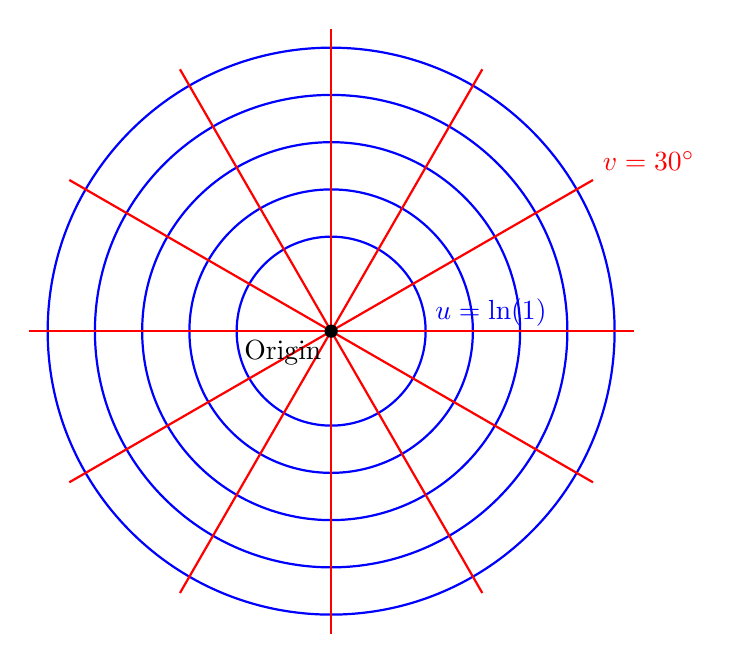
\begin{tikzpicture}[scale=1.2]
  % Draw circles: Equipotential lines for u(x,y) = ln(sqrt(x^2+y^2))
  \foreach \r in {1,1.5,2,2.5,3} {
      \draw[blue, thick] (0,0) circle (\r);
  }
  
  % Draw rays: Level sets for v(x,y) = arctan(y/x)
  \foreach \angle in {0,30,60,90,120,150,180,210,240,270,300,330} {
      \draw[red, thick] (0,0) -- (\angle:3.2);
  }
  
  % Labeling one circle and one ray to indicate the meaning
  \node[blue, right] at (1,0.2) {$u=\ln(1)$};
  \node[red, above right] at (30:3.2) {$v=30^\circ$};
  
  % Mark the origin
  \fill (0,0) circle (2pt);
  \node[below left] at (0,0) {Origin};
\end{tikzpicture}
\end{center}

\exampleline
\begin{example}
For the function \(f(z) = \Log(z)\) (with the principal branch),
\[
\Log(z)=\ln|z|+i\,\Arg(z) \quad \text{with } -\pi < \Arg(z) \le \pi,
\]
verify that the real part 
\[
u(x,y)=\ln|z|=\frac{1}{2}\ln\bigl(x^2+y^2\bigr)
\]
is harmonic.
\begin{solution}
We proceed as follows:

\begin{enumerate}
    \item Express the real part of \(\Log(z)\) in terms of \(x\) and \(y\):
    \[
    u(x,y)=\frac{1}{2}\ln(x^2+y^2).
    \]
    
    \item Compute the first partial derivatives:
    \[
    u_x=\frac{1}{2}\cdot\frac{1}{x^2+y^2}\cdot 2x=\frac{x}{x^2+y^2},\quad 
    u_y=\frac{1}{2}\cdot\frac{1}{x^2+y^2}\cdot 2y=\frac{y}{x^2+y^2}.
    \]
    
    \item Compute the second partial derivative with respect to \(x\):
    \[
    u_{xx}=\frac{\partial}{\partial x}\left(\frac{x}{x^2+y^2}\right)
    =\frac{(x^2+y^2)\cdot 1- x\cdot 2x}{(x^2+y^2)^2}
    =\frac{x^2+y^2-2x^2}{(x^2+y^2)^2}
    =\frac{y^2-x^2}{(x^2+y^2)^2}.
    \]
    
    \item Compute the second partial derivative with respect to \(y\):
    \[
    u_{yy}=\frac{\partial}{\partial y}\left(\frac{y}{x^2+y^2}\right)
    =\frac{(x^2+y^2)\cdot 1- y\cdot 2y}{(x^2+y^2)^2}
    =\frac{x^2+y^2-2y^2}{(x^2+y^2)^2}
    =\frac{x^2-y^2}{(x^2+y^2)^2}.
    \]
    
    \item Add the second derivatives:
    \[
    u_{xx}+u_{yy}=\frac{y^2-x^2}{(x^2+y^2)^2}+\frac{x^2-y^2}{(x^2+y^2)^2}=0.
    \]
    
    \item Since the Laplace equation \(u_{xx}+u_{yy}=0\) holds, \(u(x,y)=\ln|z|\) is harmonic.
\end{enumerate}
\end{solution}
\end{example}
\exampleline
\subsection*{Power Series and Analyticity} \index{Power Series}

\noindent A defining feature of holomorphic functions is their analyticity. That is, if a function \(f\) is holomorphic at a point \(z_0\), then it is equal to its Taylor series in some open disk centered at \(z_0\). More precisely, there exists a radius \(R > 0\) such that for all \(z\) with \(|z - z_0| < R\),
\[
f(z) = \sum_{n=0}^{\infty} a_n (z - z_0)^n,
\]
where the coefficients are given by the usual Taylor formula:
\[
a_n = \frac{f^{(n)}(z_0)}{n!}.
\]
This result shows that every holomorphic function is automatically infinitely differentiable, and its entire local behavior is captured by its derivatives at a single point. Within the disk of convergence, this series can be differentiated and integrated term by term, providing a powerful computational framework. \\

\noindent The analytic structure of holomorphic functions is more than a technical convenience; it reflects the rigid and highly regular nature of complex differentiability. The infinite differentiability is not just formal but constructive—convergence of the Taylor series is guaranteed in a disk where the function is holomorphic.

\exampleline
\begin{example}
Find the power series expansion of the function \(f(z) = \frac{1}{z(1 - z)}\) centered at \(z_0 = 0\), and determine its radius of convergence.
\begin{solution}
We rewrite \(f(z)\) in a form suitable for expansion. Note that
\[
f(z) = \frac{1}{z(1 - z)} = \frac{1}{z} \cdot \frac{1}{1 - z}.
\]

\begin{enumerate}
  \item Recall the geometric series expansion
  \[
  \frac{1}{1 - z} = \sum_{n=0}^{\infty} z^n \quad \text{for } |z| < 1.
  \]

  \item Multiply term by term:
  \[
  f(z) = \frac{1}{z} \cdot \sum_{n=0}^{\infty} z^n = \sum_{n=0}^{\infty} z^{n-1}.
  \]

  \item Reindex the series by letting \(m = n-1\), so that \(n = m+1\). Then the sum becomes
  \[
  f(z) = \sum_{m = -1}^{\infty} z^m.
  \]

  \item Thus, the power series expansion of \(f(z)\) about \(z_0 = 0\) is
  \[
  f(z) = \frac{1}{z} + 1 + z + z^2 + \cdots,
  \]
  valid for \(0 < |z| < 1\).

  \item The radius of convergence is \(R = 1\), but since the term \(\frac{1}{z}\) appears, the origin \(z=0\) is a simple pole. So the domain of analyticity is the punctured open disk \(0 < |z| < 1\), not the entire open disk.
\end{enumerate}
\end{solution}
\end{example}
\exampleline


\subsection*{Liouville's Theorem} \index{Liouville's Theorem}

\noindent Among the most surprising and powerful results in complex analysis (and one that seems counterintuitive when you try to visualize at first) is Liouville's Theorem. This theorem reveals a profound constraint on the behavior of entire functions—those that are holomorphic throughout the entire complex plane. An \textbf{entire function} is a function that is holomorphic (complex differentiable) at every point in the complex plane $\mathbb{C}$. Examples include polynomials, the exponential function $e^z$, and trigonometric functions like $\sin z$ and $\cos z$. Such functions are defined and analytic everywhere, with no singularities at any finite point. \\

\noindent \textbf{Liouville's Theorem:} If $f$ is an entire function and $f$ is bounded (i.e., there exists a constant $M$ such that $|f(z)| \leq M$ for all $z \in \mathbb{C}$), then $f$ must be constant. \\

\noindent This result stands in stark contrast to real analysis, where there are many non-constant functions that are both bounded and differentiable on the entire real line, such as $\sin x$, $\cos x$, $\arctan x$, and $e^{-x^2}$. In the complex domain, holomorphicity imposes a far stronger constraint—any bounded entire function must reduce to a mere constant. \\

\noindent Liouville's Theorem has profound consequences throughout complex analysis. It serves as the cornerstone for proving the Fundamental Theorem of Algebra, which guarantees that every non-constant polynomial has at least one root. It also reveals the remarkable rigidity of holomorphic functions, showing that they must either grow unboundedly as $|z| \to \infty$ or remain constant—a stark departure from the more flexible behavior permitted in real analysis.


\exampleline
\begin{example}
Use Liouville's Theorem to prove that there is no entire function $f(z)$ satisfying $|f(z)| = e^{-|z|^2}$ for all $z \in \mathbb{C}$.

\begin{solution}
\noindent We proceed by contradiction. Suppose there exists an entire function $f(z)$ such that $|f(z)| = e^{-|z|^2}$ for all $z \in \mathbb{C}$. First, observe that $e^{-|z|^2}$ is bounded for all $z \in \mathbb{C}$. In fact: \( 0 < e^{-|z|^2} \leq 1 \quad \text{for all } z \in \mathbb{C} \) with the maximum value of 1 occurring at $z = 0$. Since $|f(z)| = e^{-|z|^2}$, we know that $f$ is also bounded, with:
\[
|f(z)| \leq 1 \quad \text{for all } z \in \mathbb{C}
\]

\noindent By Liouville's Theorem, any bounded entire function must be constant. Therefore, $f(z) = C$ for some constant $C$. \\

\noindent But if $f$ is constant, then $|f(z)| = |C|$ for all $z \in \mathbb{C}$. This contradicts our original assumption that $|f(z)| = e^{-|z|^2}$, because $e^{-|z|^2}$ is not constant (it varies with $|z|$). Therefore, no such entire function exists.
\end{solution}
\end{example}
\exampleline


\subsection*{Connection to Conformal Mapping} \index{Conformal Mapping}

\noindent A fundamental consequence of complex differentiability is that, wherever the derivative \(f'(z_0)\neq 0\), the function \(f\) acts as a local \textbf{conformal map}. In other words, not only does \(f\) possess a linear approximation
\[
f(z) \approx f(z_0) + f'(z_0)(z - z_0),
\]
but this approximation has a very special geometric interpretation: the complex number \(f'(z_0)\) acts as a scaling and rotation factor. Specifically, the modulus \(|f'(z_0)|\) scales infinitesimal distances (i.e., stretches or compresses small figures) and the argument \(\arg(f'(z_0))\) rotates them. Consequently, if two curves intersect at \(z_0\) with an angle \(\theta\), then their images under \(f\) will intersect at \(f(z_0)\) with the same angle \(\theta\). \\

\noindent The following diagram illustrates this property. In the \(z\)-plane (left), two curves intersect at \(z_0\); dashed lines represent the tangent directions at \(z_0\) and a small arc between these lines marks the angle \(\theta\) between them. Under the mapping \(f\), these curves are transformed in the \(w\)-plane (right) with the same relative angle preserved.

\begin{figure}[H]
\centering
\begin{tikzpicture}[scale=1.3]

% -------------- z-plane (original curves) --------------
\begin{scope}
  % Axes for z-plane
  \draw[->] (-2,0) -- (2,0) node[right] {\(\text{Re}(z)\)};
  \draw[->] (0,-2) -- (0,2) node[above] {\(\text{Im}(z)\)};
  
  % Two original curves (dotted) intersecting at z_0
  \draw[dotted, thick] (-1.8,-1.5) .. controls (-0.5,0) .. (1.5,1);
  \draw[dotted, thick] (-1.2,1.4) .. controls (0.2,0) .. (1.8,-1.2);
  
  % Intersection point z_0
  \fill (0,0) circle (1.5pt) node[below left] {\(z_0\)};
  
  % Draw red angle arc for the original curves
  \draw[red, thick] (0.9,0) arc (0:40:0.9);
  \node[red] at (1.0,0.45) {\(\theta\)};
  
  \node at (0,-2.3) {Original curves at \(z_0\)};
\end{scope}

% ---------------- Mapping arrow ----------------
\begin{scope}[shift={(3,0)}]  % Adjust shift here to modify spacing.
  \draw[->, thick] (0,0) -- (1.5,0) node[midway, above] {\(f\)};
\end{scope}

% -------------- w-plane (mapped curves) --------------
\begin{scope}[shift={(7,0)}]  % Adjust shift here to modify spacing.
  % Axes for w-plane
  \draw[->] (-2,0) -- (2,0) node[right] {\(\text{Re}(w)\)};
  \draw[->] (0,-2) -- (0,2) node[above] {\(\text{Im}(w)\)};
  
  % Mapped curves: slightly perturbed to illustrate a nontrivial conformal map (e.g. \(f(z)=z+z^2\))
  \draw[thick] (-1.8,-1.3) .. controls (-0.3,0.5) .. (1.3,0.8);
  \draw[thick] (-1.0,1.6) .. controls (0.6,0.2) .. (1.8,-0.9);
  
  % Mapped intersection point f(z_0)
  \fill (0,0) circle (1.5pt) node[below left] {\(f(z_0)\)};
  
  % Draw blue angle arc for the mapped curves
  \draw[blue, thick] (0.9,0) arc (0:47:0.9);
  \node[blue] at (1.3,0.45) {\(\theta'=\theta\)};
  
  \node at (0,-2.3) {Mapped curves at \(f(z_0)\)};
\end{scope}

\end{tikzpicture}
\caption{\textit{A conformal mapping \(f\) (e.g. \(f(z)=z+z^2\) near \(z_0\)) transforms the original curves in the \(z\)-plane (left) into modified curves in the \(w\)-plane (right). The red angle arc in the \(z\)-plane and the blue angle arc in the \(w\)-plane both measure \(\theta\), illustrating that \(f\) preserves the angle between intersecting curves.}}
\label{fig:conformal-map}
\end{figure}


\newpage

\lecture{Elementary Complex Integration} \index{Complex Integration}

\noindent Complex integration extends the familiar concept of integration from calculus to the complex plane, allowing us to evaluate integrals along paths rather than just intervals. In Chapter 5, Lecture 2, we studied line integrals in the context of vector fields in $\mathbb{R}^n$; complex integration builds upon these concepts but adds powerful new structures unique to complex analysis. This seemingly straightforward extension leads to surprisingly powerful results that form the cornerstone of complex analysis. In this lecture, we will develop the theory of complex integration, explore its geometric meaning, and establish key properties that will serve as the foundation for the elegant theorems to follow.

\subsection*{Path Integrals in the Complex Plane} \index{Path Integrals}

\noindent In real calculus, we integrate functions over intervals. In complex analysis, we integrate functions along paths or curves in the complex plane, similar to the line integrals we studied earlier, but with the added richness of complex function theory. As we'll see, the requirement of holomorphicity imposes much stronger conditions on complex integrals than we observed with real vector fields, leading to remarkable consequences.

\subsubsection*{Parametrization of Curves}

\noindent To precisely define integration along a curve, we first need to formalize the concept of a curve in the complex plane. A \textbf{parametrized curve} (or \textbf{path}) $\gamma$ is a continuous function that maps a real interval $[a,b]$ to points in the complex plane:
\[
\gamma: [a,b] \to \mathbb{C}
\]

\noindent We often express the curve parametrically as $\gamma(t) = x(t) + iy(t)$ for $t \in [a,b]$, where $x(t)$ and $y(t)$ are real-valued continuous functions representing the real and imaginary parts, respectively. This should be familiar from our work with parametrized curves in vector calculus. \\

\noindent A curve $\gamma$ is said to be \textbf{piecewise smooth} if its component functions $x(t)$ and $y(t)$ have continuous derivatives except possibly at finitely many points. A \textbf{smooth curve} has continuous derivatives throughout its domain. These conditions ensure that the curve behaves well enough for integration purposes. \\

\noindent The derivative of a curve is denoted by $\gamma'(t) = x'(t) + iy'(t)$, and it represents the velocity vector along the curve at time $t$. This derivative plays a crucial role in defining the complex line integral, as it provides the direction and rate of traversal along the path. \\

\noindent A curve $\gamma$ is \textbf{simple} if it does not intersect itself, except possibly at its endpoints. When $\gamma(a) = \gamma(b)$, we say the curve is \textbf{closed}. \\

\noindent The \textbf{length} of a piecewise smooth curve $\gamma$ over $[a,b]$ is given by:
\[
L(\gamma) = \int_a^b |\gamma'(t)| \, dt = \int_a^b \sqrt{[x'(t)]^2 + [y'(t)]^2} \, dt
\]

\noindent Different parametrizations can represent the same geometric curve. For instance, if $\phi: [c,d] \to [a,b]$ is a strictly increasing, continuously differentiable function with $\phi(c) = a$ and $\phi(d) = b$, then $\gamma \circ \phi$ is a reparametrization of $\gamma$. The physical curve is the same, but the "speed" at which we traverse it may differ.



\subsubsection*{Definition of the Complex Line Integral} \index{Complex Line Integral}

\noindent Given a complex-valued function $f(z) = u(x,y) + iv(x,y)$ defined on a region containing a piecewise smooth curve $\gamma: [a,b] \to \mathbb{C}$, the \textbf{complex line integral} of $f$ along $\gamma$ is defined as:
\[
\int_{\gamma} f(z) \, dz = \int_a^b f(\gamma(t)) \, \gamma'(t) \, dt
\]

\noindent This definition requires both $f$ and $\gamma$ to be well-behaved, with $f$ being continuous along the curve and $\gamma$ being piecewise smooth. The integral combines the function value at each point with the derivative of the curve, creating a sort of ``weighted average" of the function along the path. \\

\begin{figure}[H]
\centering
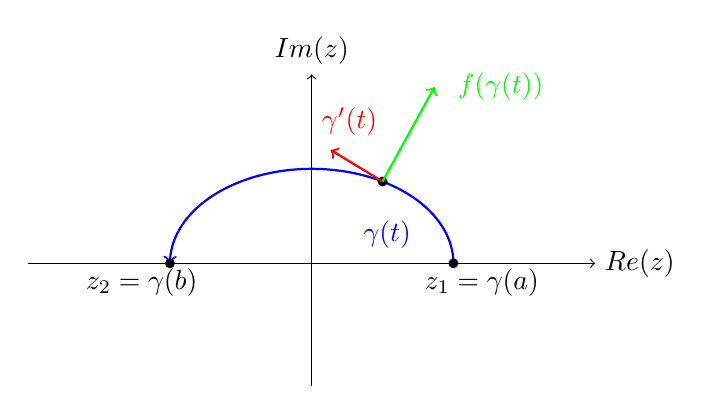
\begin{tikzpicture}[scale=1.2]
    % Draw axes
    \draw[->] (-3,0) -- (3,0) node[right] {$\text{Re}(z)$};
    \draw[->] (0,-1.3) -- (0,2) node[above] {$\text{Im}(z)$};
    
    % Draw a path (parametric curve)
    \draw[thick, blue, ->] plot[domain=0:3.14, samples=100] ({1.5*cos(\x r)}, {sin(\x r)});
    
    % Add points and labels with explicit coordinates
    \fill (1.5,0) circle (1.5pt);
    \node at (1.8,-0.2) {$z_1=\gamma(a)$};
    
    \fill (-1.5,0) circle (1.5pt);
    \node at (-1.8,-0.2) {$z_2=\gamma(b)$};
    
    % Point on curve
    \fill (0.75,0.866) circle (1.5pt);
    \node at (0.75,0.5) {$$};
    
    % Add tangent vector at a point
\draw[->, thick, red] (0.75,0.866) -- (0.2,1.2);
    \node[red] at (0.4,1.5) {$\gamma'(t)$};
    
    % Label the curve
    \node[blue] at (0.8,0.3) {$\gamma(t)$};
    
    % Function value at a point (represented as a vector)
\draw[->, thick, green] (0.75,0.866) -- (1.3,1.866);
    \node[green] at (2.0,1.866) {$f(\gamma(t))$};
    
\end{tikzpicture}
\caption{\textit{A geometric representation of a complex line integral. The function $f(z)$ (green vector) is evaluated at each point along the path $\gamma$ (blue curve) and multiplied by the tangent vector $\gamma'(t)$ (red) before integration.}}
\label{fig:complex-line-integral}
\end{figure}

\noindent To understand this definition more clearly, let's express it in terms of real and imaginary parts. Let $f(z) = u(x,y) + iv(x,y)$ and $\gamma(t) = x(t) + iy(t)$. Then:
\begin{align*}
\int_{\gamma} f(z) \, dz &= \int_a^b f(\gamma(t)) \, \gamma'(t) \, dt \\
&= \int_a^b [u(x(t),y(t)) + iv(x(t),y(t))] \, [x'(t) + iy'(t)] \, dt \\
&= \int_a^b [u \cdot x' - v \cdot y' + i(u \cdot y' + v \cdot x')] \, dt \\
\end{align*}

\noindent This expression highlights that the complex line integral combines the real and imaginary parts of the function in a specific way that accounts for both the function's values and the curve's direction. \\

\noindent For computational purposes, we can write:
\begin{align*}
\int_{\gamma} f(z) \, dz = \int_a^b [u(x(t),y(t)) \cdot x'(t) - v(x(t),y(t)) \cdot y'(t)] \, dt \\
+ i\int_a^b [u(x(t),y(t)) \cdot y'(t) + v(x(t),y(t)) \cdot x'(t)] \, dt
\end{align*}

\noindent When $\gamma$ is a segment along the real axis from $a$ to $b$, parametrized as $\gamma(t) = t$ for $t \in [a,b]$, the complex line integral reduces to the familiar real integral:
\[
\int_{\gamma} f(z) \, dz = \int_a^b f(t) \, dt
\]
which connects complex integration to the real integrals we've studied previously. You can use this list of common parameterizations to aid you. Some of the parameterizations like a circle or arc are a little bit different compared to their real counterpart.

\begin{table}[htb]
\caption{Common Parameterizations for Complex Line Integrals}
\begin{center}
\small
\begin{tabular}{|p{2.5cm}|p{4.5cm}|p{3cm}|p{3.5cm}|}
\hline
\rule{0pt}{4ex}\textbf{Curve Type} & \textbf{Complex Parameterization} & \textbf{Parameter Range} & \textbf{Derivative $\gamma'(t)$} \rule[-2ex]{0pt}{0pt}\\
\hline
\rule{0pt}{4ex}Line Segment &
$\gamma(t) = z_1 + t(z_2-z_1)$ &
$0 \leq t \leq 1$ &
$\gamma'(t) = z_2 - z_1$ \rule[-2ex]{0pt}{0pt}\\
\hline
\rule{0pt}{4ex}Circle/Arc &
$\gamma(t) = z_0 + re^{it}$ &
$\alpha \leq t \leq \beta$ &
$\gamma'(t) = ire^{it}$ \rule[-2ex]{0pt}{0pt}\\
\hline
\rule{0pt}{4ex}Ellipse &
$\gamma(t) = z_0 + a\cos t + ib\sin t$ &
$0 \leq t \leq 2\pi$ &
$\gamma'(t) = -a\sin t + ib\cos t$ \rule[-2ex]{0pt}{0pt}\\
\hline
\rule{0pt}{4ex}Ray/Radial Line &
$\gamma(t) = z_0 + te^{i\theta}$ &
$0 \leq t \leq R$ &
$\gamma'(t) = e^{i\theta}$ \rule[-2ex]{0pt}{0pt}\\
\hline
\rule{0pt}{4ex}Rectangular Contour &
$\gamma_1 \cup \gamma_2 \cup \gamma_3 \cup \gamma_4$ &
Piecewise definition &
Piecewise constant \rule[-2ex]{0pt}{0pt}\\
\hline
\end{tabular}
\end{center}
\label{tab:complex-curve-parameterizations}
\end{table}

\exampleline
\begin{example}
Evaluate the complex line integral $\displaystyle\int_{\gamma} z^2 \, dz$ where $\gamma$ is the straight line segment from $z_1 = 1+i$ to $z_2 = 3+4i$.

\begin{solution}
We proceed step by step to evaluate this integral:

\begin{enumerate}
\item First, we parametrize the straight line from $z_1$ to $z_2$. A natural parametrization is:
   \[
   \gamma(t) = (1-t)(1+i) + t(3+4i) = 1+i + t(2+3i), \quad t \in [0,1]
   \]
   Simplifying:
   \[
   \gamma(t) = (1+2t) + i(1+3t), \quad t \in [0,1]
   \]

\item The derivative of the path is:
   \[
   \gamma'(t) = 2 + 3i
   \]

\item We evaluate $f(\gamma(t))$ where $f(z) = z^2$:
   \begin{align*}
   f(\gamma(t)) &= \Big[(1+2t) + i(1+3t)\Big]^2 \\
   &= (1+2t)^2 - (1+3t)^2 + 2i(1+2t)(1+3t) \\
   &= \Big[(1+4t+4t^2) - (1+6t+9t^2)\Big] + 2i(1+5t+6t^2) \\
   &= (-2t-5t^2) + 2i(1+5t+6t^2)
   \end{align*}

\item Now we compute the integral:
   \begin{align*}
   \int_{\gamma} z^2 \, dz &= \int_0^1 f(\gamma(t))\, \gamma'(t)\, dt \\
   &= \int_0^1 \Big[(-2t-5t^2) + 2i(1+5t+6t^2)\Big](2+3i)\, dt.
   \end{align*}
   
   Multiplying:
   \begin{align*}
   &\Big[(-2t-5t^2) + 2i(1+5t+6t^2)\Big](2+3i) \\
   &= (-2t-5t^2)(2+3i) + 2i(1+5t+6t^2)(2+3i) \\
   &= \Big[-4t-10t^2 - 6it-15it^2\Big] + \Big[-6-30t-36t^2 + 4i+20it+24it^2\Big] \\
   &= \Big[-6 - 34t - 46t^2\Big] + i\Big[4 + 14t + 9t^2\Big]
   \end{align*}

\item Finally, we integrate with respect to $t$:
   \begin{align*}
   \int_{\gamma} z^2 \, dz &= \int_0^1 \Big[-6 - 34t - 46t^2 + i(4 + 14t + 9t^2)\Big] dt \\
   &= \Big[-6t - 17t^2 - \frac{46}{3}t^3 + i\Big(4t + 7t^2 + 3t^3\Big)\Big]_0^1 \\
   &= -6 - 17 - \frac{46}{3} + i(4+7+3) \\
   &= -\frac{115}{3} + 14i.
   \end{align*}

Therefore, 
\[
\displaystyle\int_{\gamma} z^2 \, dz = -\frac{115}{3} + 14i.
\]
\end{enumerate}
\end{solution}
\end{example}
\exampleline


\subsubsection*{Alternative Forms and Notation}

\noindent There are several common notations for complex line integrals. If $\gamma$ is a curve from point $z_1$ to $z_2$, we might write:
\[
\int_{\gamma} f(z) \, dz \quad \text{or} \quad \int_{z_1}^{z_2} f(z) \, dz \quad \text{or} \quad \int_{C} f(z) \, dz
\]

\noindent When the curve is closed, we sometimes use the notation:
\[
\oint_{\gamma} f(z) \, dz
\]
where the circle in the integral sign emphasizes that we're integrating around a closed contour.

\begin{figure}[H]
\centering
\begin{tikzpicture}[scale=1.2]
% Draw axes
\draw[->] (-3,0) -- (3,0) node[right] {$\text{Re}(z)$};
\draw[->] (0,-3) -- (0,2.5) node[above] {$\text{Im}(z)$};

% Draw a simple path (line segment)
\draw[thick, blue, ->] (-2,1) -- (2,-1);
\fill (-2,1) circle (1.5pt) node[above left] {$z_1$};
\fill (2,-1) circle (1.5pt) node[below right] {$z_2$};
% Separate label for gamma_1 with explicit coordinates
\node[blue] at (-0.8,0.7) {$\gamma_1$};

% Draw a closed contour (circle)
\draw[thick, red, ->] (0,-1.5) circle (1cm);
% Separate label for gamma_2 with explicit coordinates
\node[red] at (1.3,-1.5) {$\gamma_2$};

% Draw a piecewise path
\draw[thick, green, ->] (-2.5,-1) -- (-1,-1);
\draw[thick, green, ->] (-1,-1) -- (0,0.5) -- (1.5,0.5);
\fill (-2.5,-1) circle (1.5pt) node[left] {$z_3$};
\fill (1.5,0.5) circle (1.5pt) node[right] {$z_4$};
% Separate label for gamma_3 with explicit coordinates
\node[green] at (-0.8,-.3) {$\gamma_3$};

\end{tikzpicture}
\caption{\textit{Various types of paths in the complex plane: a simple curve $\gamma_1$ (blue), a closed contour $\gamma_2$ (red), and a piecewise curve $\gamma_3$ (green). Each path requires appropriate notation and treatment when computing complex line integrals.}}
\label{fig:integration-paths}
\end{figure}

\noindent For a curve parametrized as $z = z(t)$, we sometimes write:
\[
\int_{\gamma} f(z) \, dz = \int_a^b f(z(t)) \, z'(t) \, dt
\]

\noindent In vector calculus terms, if we denote $\mathbf{r}(t) = (x(t), y(t))$ as the position vector in the complex plane, and $f(z) = P(x,y) + iQ(x,y)$, then:
\[
\int_{\gamma} f(z) \, dz = \int_{\gamma} (P + iQ) \, d(x + iy) = \int_{\gamma} P \, dx - Q \, dy + i\int_{\gamma} Q \, dx + P \, dy
\]

\noindent This relates the complex line integral to the line integrals of vector fields we studied in vector calculus.

\exampleline
\begin{example}
Evaluate the complex line integral $\displaystyle\int_{\gamma} \bar{z} \, dz$ where $\gamma$ is the unit circle $|z| = 1$ traversed once counterclockwise.

\begin{solution}
We need to parametrize the unit circle and apply the definition of the complex line integral.

\begin{enumerate}
\item Parametrize the unit circle:
   \[
   \gamma(t) = e^{it}, \quad t \in [0, 2\pi]
   \]
   
   The derivative is:
   \[
   \gamma'(t) = ie^{it}
   \]

\item For $z = e^{it}$, the complex conjugate is:
   \[
   \bar{z} = \overline{e^{it}} = e^{-it}
   \]

\item Now we compute the integrand:
   \[
   f(\gamma(t)) \cdot \gamma'(t) = e^{-it} \cdot ie^{it} = i
   \]
   
   Notice that this simplifies to a constant.

\item Evaluating the integral:
   \begin{align*}
   \int_{\gamma} \bar{z} \, dz &= \int_0^{2\pi} e^{-it} \cdot ie^{it} \, dt \\
   &= \int_0^{2\pi} i \, dt \\
   &= i \cdot 2\pi \\
   &= 2\pi i
   \end{align*}
\end{enumerate}

Therefore, $\displaystyle\int_{\gamma} \bar{z} \, dz = 2\pi i$ when $\gamma$ is the unit circle traversed counterclockwise.

\noindent This example illustrates an important point: even for a function like $\bar{z}$ that is not holomorphic, the integral around a closed curve need not be zero. As we'll see later in the chapter, this contrasts with holomorphic functions, for which integrals around closed curves in appropriate domains vanish.
\end{solution}
\end{example}
\exampleline










\subsection*{Basic Properties of Complex Line Integrals} \index{Properties of Complex Integrals}

\noindent Complex line integrals inherit many properties from real integrals while also exhibiting some distinctive features due to their path-dependent nature.

\subsubsection*{Linearity}

\noindent For any complex-valued functions $f$ and $g$ that are continuous along a piecewise smooth curve $\gamma$, and for any complex constants $\alpha$ and $\beta$:
\[
\int_{\gamma} [\alpha f(z) + \beta g(z)] \, dz = \alpha \int_{\gamma} f(z) \, dz + \beta \int_{\gamma} g(z) \, dz
\]

\noindent This property follows directly from the linearity of real integrals and allows us to break down complex integrals into simpler components.

\subsubsection*{Additivity with Respect to Paths}

\noindent If a curve $\gamma$ is composed of two curves $\gamma_1$ and $\gamma_2$ joined end-to-end (i.e., the endpoint of $\gamma_1$ is the starting point of $\gamma_2$), then:
\[
\int_{\gamma} f(z) \, dz = \int_{\gamma_1} f(z) \, dz + \int_{\gamma_2} f(z) \, dz
\]

\noindent This property allows us to evaluate complex integrals by breaking the path into simpler segments.

\subsubsection*{Reverse Orientation}

\noindent If $-\gamma$ denotes the curve $\gamma$ traversed in the opposite direction, then:
\[
\int_{-\gamma} f(z) \, dz = -\int_{\gamma} f(z) \, dz
\]

\noindent This property reflects the fact that reversing the path direction negates the line integral. If $\gamma$ is parametrized by $\gamma(t)$ for $t \in [a,b]$, then $-\gamma$ can be parametrized as $(-\gamma)(t) = \gamma(a+b-t)$ for $t \in [a,b]$.

\subsubsection*{ML Inequality} \index{ML Inequality}

\noindent If $f$ is continuous on a piecewise smooth curve $\gamma$, then we have the following estimate:
\[
\left| \int_{\gamma} f(z) \, dz \right| \leq L(\gamma) \cdot \max_{z \in \gamma} |f(z)|
\]
where $L(\gamma)$ is the length of the curve. This inequality, often called the ML inequality (where M stands for the maximum value of $|f|$ and L for the path length), provides an upper bound for the magnitude of the complex line integral. \\

\noindent The ML inequality is particularly useful for estimating the size of complex integrals without explicitly evaluating them, which becomes important when studying convergence of series of complex integrals or when establishing bounds for error terms. \\

\noindent To prove this inequality, we use the definition of the complex line integral and basic properties of real integrals:
\begin{align*}
\left| \int_{\gamma} f(z) \, dz \right| &= \left| \int_a^b f(\gamma(t)) \, \gamma'(t) \, dt \right| \\
&\leq \int_a^b |f(\gamma(t))| \, |\gamma'(t)| \, dt \\
&\leq \max_{t \in [a,b]} |f(\gamma(t))| \cdot \int_a^b |\gamma'(t)| \, dt \\
&= \max_{z \in \gamma} |f(z)| \cdot L(\gamma)
\end{align*}







\subsection*{Integration of Specific Types of Functions}

\noindent Certain categories of complex functions have special integration properties that are worth highlighting.

\subsubsection*{Integration of Powers and Polynomials}

\noindent For simple curves like line segments or circular arcs, we can often compute integrals of powers of $z$ directly. For instance, on a line segment from $z_1$ to $z_2$ parametrized as $\gamma(t) = (1-t)z_1 + tz_2$ for $t \in [0,1]$, we have:
\[
\int_{\gamma} z^n \, dz = \frac{z_2^{n+1} - z_1^{n+1}}{n+1} \quad \text{for } n \neq -1
\]

\noindent For $n = -1$, the integral of $\frac{1}{z}$ depends on the path and will be discussed in the context of logarithmic functions and multi-valued functions. For polynomials $P(z) = a_0 + a_1z + a_2z^2 + \cdots + a_nz^n$, we can integrate term by term using linearity:
\[
\int_{\gamma} P(z) \, dz = a_0 \int_{\gamma} dz + a_1 \int_{\gamma} z \, dz + \cdots + a_n \int_{\gamma} z^n \, dz
\]

\subsubsection*{Integration of Rational Functions}

\noindent Rational functions, which are quotients of polynomials, are integrated using techniques like partial fraction decomposition, similar to real calculus. The approach breaks down the rational function into simpler terms that can be integrated individually. \\

\noindent For instance, a rational function of the form $\frac{P(z)}{(z-a)^n}$ where $P(z)$ is a polynomial and $(z-a)^n$ is a factor in the denominator, contributes terms involving logarithms (for $n=1$) or negative powers of $(z-a)$ (for $n>1$) in the antiderivative.

\subsubsection*{Integration of Trigonometric and Exponential Functions}

\noindent The complex exponential function $e^z$ integrates to itself, similar to the real case:
\[
\int_{\gamma} e^z \, dz = \left. e^z \right|_{\gamma_{\text{start}}}^{\gamma_{\text{end}}} = e^{\gamma_{\text{end}}} - e^{\gamma_{\text{start}}}
\]
assuming the integral is taken along a simple curve.

\noindent Since the complex trigonometric functions are defined in terms of complex exponentials, their integrals follow familiar patterns from real calculus:
\begin{align*}
\int_{\gamma} \sin z \, dz &= \left. -\cos z \right|_{\gamma_{\text{start}}}^{\gamma_{\text{end}}} \\
\int_{\gamma} \cos z \, dz &= \left. \sin z \right|_{\gamma_{\text{start}}}^{\gamma_{\text{end}}}
\end{align*}

\exampleline
\begin{example}
Let \( k > 0 \) be given, and for each \( R > 0 \) define the closed contour
\(
\Gamma_R = \gamma_1 \cup \gamma_2,
\)
where 
\begin{enumerate}
    \item \(\gamma_1\) is the line segment along the real axis from \(-R\) to \(R\),
    \item \(\gamma_2\) is the upper semicircular arc from \(R\) to \(-R\), parameterized by 
    \( z(t)=Re^{it},\; t\in[0,\pi] \).
\end{enumerate}
Show that 
\(
\lim_{R\to\infty}\int_{\gamma_2} e^{ikz}\,dz = 0,
\)
using the ML inequality and the additivity and linearity of the integral, and explain the role of the \(\gamma_1\) part.

\begin{solution}
We first parameterize \(\gamma_2\) by 
\(
z(t)=Re^{it},\; dz=iRe^{it}\,dt,\; t\in[0,\pi].
\)
Then,
\[
\int_{\gamma_2} e^{ikz}\,dz = \int_0^{\pi} e^{ikRe^{it}}\, iRe^{it}\,dt.
\]
Taking absolute values and applying the ML inequality,
\[
\left|\int_{\gamma_2} e^{ikz}\,dz\right| \le R\int_0^{\pi}\left|e^{ikRe^{it}}\right|dt.
\]
Since 
\(
e^{ikRe^{it}} = e^{ikR(\cos t + i\sin t)} = e^{ikR\cos t}\,e^{-kR\sin t}
\)
and hence 
\(
\left|e^{ikRe^{it}}\right| = e^{-kR\sin t},
\)
we obtain
\[
\left|\int_{\gamma_2} e^{ikz}\,dz\right| \le R\int_0^\pi e^{-kR\sin t}\,dt.
\]
Letting 
\(
J(R)=\int_0^\pi e^{-kR\sin t}\,dt,
\)
we estimate \(J(R)\) as follows: For any fixed \(\epsilon\in(0,\tfrac{\pi}{2})\),
\begin{itemize}
    \item For \(t\in[\epsilon,\pi-\epsilon]\), \(\sin t\ge\sin\epsilon\) so that
    \[
    \int_{\epsilon}^{\pi-\epsilon} e^{-kR\sin t}\,dt \le (\pi-2\epsilon)e^{-kR\sin\epsilon}.
    \]
    \item For \(t\in[0,\epsilon]\) (and similarly near \(\pi\)), using \(\sin t\ge t/2\) gives
    \[
    \int_{0}^{\epsilon} e^{-kR\sin t}\,dt \le \int_0^{\epsilon} e^{-kRt/2}\,dt = \frac{2}{kR}\Bigl(1-e^{-kR\epsilon/2}\Bigr).
    \]
\end{itemize}
Thus, \( J(R) \) decays at least as \( O(1/R) \) and exponentially on the middle interval, so that 
\(
R\cdot J(R)\to0 \) as \( R\to\infty.
\)
Hence,
\[
\lim_{R\to\infty}\int_{\gamma_2} e^{ikz}\,dz = 0.
\]

Now, consider \(\gamma_1\). Parameterizing by \( z=x \) with \( x\in[-R,R] \) (so \(dz=dx\)), we have
\[
\int_{\gamma_1} e^{ikz}\,dz = \int_{-R}^{R} e^{ikx}\,dx.
\]
Since \( e^{ikz} \) is entire, Cauchy's theorem tells us that 
\(
\int_{\Gamma_R} e^{ikz}\,dz = 0.
\)
Thus, by additivity,
\[
\int_{-R}^{R} e^{ikx}\,dx = -\int_{\gamma_2} e^{ikz}\,dz.
\]
Taking the limit as \( R\to\infty \) and noting that the arc contribution vanishes, we obtain
\[
\lim_{R\to\infty}\int_{-R}^{R} e^{ikx}\,dx = 0.
\]
This analysis of both \(\gamma_2\) and \(\gamma_1\) is a key step in many contour integration techniques used to evaluate real integrals via complex methods.

\end{solution}
\end{example}
\exampleline



\subsection*{Antiderivatives and Path Independence} \index{Antiderivatives} \index{Path Independence}

\noindent One of the most significant results in complex integration is the fact that under certain conditions, a complex line integral becomes independent of the specific path taken between two points, depending only on the endpoints. This property leads to the concept of antiderivatives in the complex plane.

\subsubsection*{Antiderivatives in the Complex Plane}

\noindent A function $F(z)$ is called an \textbf{antiderivative} (or \textbf{primitive}) of $f(z)$ on a domain $D$ if $F'(z) = f(z)$ for all $z \in D$. When an antiderivative exists on a suitable domain, it allows us to compute complex line integrals using a formula analogous to the Fundamental Theorem of Calculus. Specifically, if $f(z)$ has an antiderivative $F(z)$ on a domain containing a piecewise smooth curve $\gamma$ from $z_1$ to $z_2$, then:
\[
\int_{\gamma} f(z) \, dz = F(z_2) - F(z_1)
\]

\noindent This powerful result means that when an antiderivative exists, the complex line integral depends only on the endpoints of the path, not on the specific path taken between them.

\subsubsection*{Path Independence and Simply Connected Domains}

\noindent A complex line integral $\int_{\gamma} f(z) \, dz$ is \textbf{path-independent} in a domain $D$ if its value depends only on the endpoints of the path, not on the specific path taken. Path independence is equivalent to the existence of an antiderivative: The integral $\int_{\gamma} f(z) \, dz$ is path-independent in $D$ if and only if $f(z)$ has an antiderivative in $D$. \\

\noindent Path independence is closely linked to \textbf{simply connected domains} – domains where every simple closed curve can be continuously shrunk to a point while staying within the domain (intuitively, domains without "holes"). For a continuous function $f(z)$ on a simply connected domain $D$, the following are equivalent:
\begin{enumerate}
\item $f(z)$ has an antiderivative in $D$.
\item $\int_{\gamma} f(z) \, dz$ is path-independent in $D$.
\item For every simple closed curve $\gamma$ in $D$, $\oint_{\gamma} f(z) \, dz = 0$.
\end{enumerate}

\subsubsection*{Multiply Connected Domains and Winding Numbers} \index{Multiply Connected Domains} \index{Winding Number}

\noindent A domain that is not simply connected is called \textbf{multiply connected}. Such domains contain "holes" that can create path-dependent integrals, even for holomorphic functions. \\

\noindent The \textbf{winding number} of a closed curve $\gamma$ with respect to a point $a$ (not on $\gamma$), denoted $n(\gamma,a)$, counts how many times $\gamma$ encircles the point $a$ in the counterclockwise direction. For a simple closed counterclockwise curve, the winding number is 1 for points inside the curve and 0 for points outside. \\

\noindent For example, in the punctured plane $\mathbb{C} \setminus \{0\}$, the function $f(z) = \frac{1}{z}$ is holomorphic, but the integral $\int_{\gamma} \frac{1}{z} \, dz$ depends on the winding number of $\gamma$ around the origin:
\[
\oint_{\gamma} \frac{1}{z} \, dz = 2\pi i \cdot n(\gamma,0)
\]

\noindent This formula reveals that the integral equals $2\pi i$ multiplied by the number of counterclockwise revolutions around the origin (negative if clockwise). These quantities, called \textbf{periods}, are fundamental in the study of Riemann surfaces and multi-valued functions like the logarithm.

\exampleline
\begin{example}
Evaluate $\oint_{\gamma} \frac{1}{z}\,dz$ where $\gamma$ is a closed path that winds twice around the origin counterclockwise.

\begin{solution}
\begin{enumerate}
\item The winding number of $\gamma$ around the origin is $n(\gamma,0) = 2$.

   \begin{figure}[H]
   \centering
   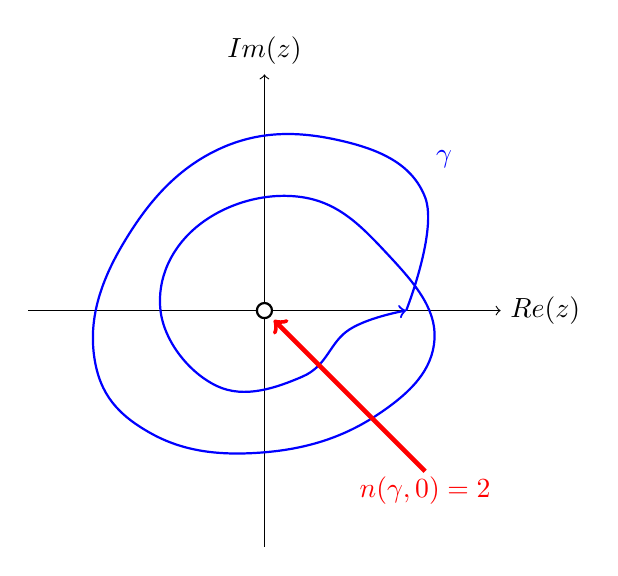
\begin{tikzpicture}[scale=1.2]
      % Draw axes
      \draw[->] (-2.5,0) -- (2.5,0) node[right] {$\text{Re}(z)$};
      \draw[->] (0,-2.5) -- (0,2.5) node[above] {$\text{Im}(z)$};
      
      % Mark the origin as a puncture
      \fill[white] (0,0) circle (0.08);
      \draw[thick] (0,0) circle (0.08);
      
      % Draw a freehand-style path that winds twice around the origin
      \draw[thick, blue, ->] plot[smooth, tension=0.7] 
        coordinates {(1.5,0) (1.7,1.2) (0.8,1.8) (-0.5,1.7) (-1.5,0.7) 
                    (-1.8,-0.5) (-1.2,-1.3) (0,-1.5) (1.2,-1.1) (1.8,-0.3)
                    (1.3,0.6) (0.4,1.2) (-0.7,0.9) (-1.1,0) (-0.5,-0.8)
                    (0.4,-0.7) (0.9,-0.2) (1.5,0)};
      
      % Add a spiral dial indicator pointing to the origin
      \draw[->, ultra thick, red] plot[smooth, tension=0.7] 
        coordinates {(1.7,-1.7) (1.2,-1.2) (0.8,-0.8) (0.5,-0.5) (0.3,-0.3) (0.1,-0.1)};
      
      % Add annotations
      \node[blue] at (1.9,1.6) {$\gamma$};
      \node[red] at (1.7,-1.9) {$n(\gamma,0)=2$};
   \end{tikzpicture}
   \caption{\textit{A freehand closed contour $\gamma$ with winding number 2 around the origin. The spiral dial indicator shows how the path winds twice around the origin before closing.}}
   \label{fig:double-winding}
   \end{figure}

\item Using the winding number formula:
   \[
   \oint_{\gamma} \frac{1}{z}\,dz = 2\pi i \cdot n(\gamma,0) = 2\pi i \cdot 2 = 4\pi i
   \]

\item This confirms that the integral value is directly proportional to the winding number, demonstrating the path dependence in the multiply connected domain $\mathbb{C} \setminus \{0\}$.
\end{enumerate}
\end{solution}
\end{example}
\exampleline

\subsection*{Fundamental Theorem for Line Integrals (Revisited)} \index{Fundamental Theorem for Line Integrals}

\noindent In vector calculus, we learned that if $\mathbf{F} = \nabla \phi$ is a conservative vector field (i.e., the gradient of a scalar potential $\phi$), then the line integral of $\mathbf{F}$ along any curve depends only on the endpoints:
\[
\int_{\gamma} \mathbf{F} \cdot d\mathbf{r} = \phi(P_2) - \phi(P_1)
\]
where $P_1$ and $P_2$ are the endpoints of the curve. The complex analog of this result states that if $f(z)$ has an antiderivative $F(z)$ in a domain $D$, then for any piecewise smooth curve $\gamma$ in $D$ with endpoints $z_1$ and $z_2$:
\[
\int_{\gamma} f(z) \, dz = F(z_2) - F(z_1)
\]

\noindent As in vector calculus, this result is known as the Fundamental Theorem for Line Integrals. It provides a powerful computational tool, allowing us to evaluate complex line integrals without performing the actual integration along the path. The Fundamental Theorem also has a special case for closed curves (i.e., curves where the starting and ending points coincide). If $\gamma$ is a closed curve in a domain where $f(z)$ has an antiderivative, then:
\[
\oint_{\gamma} f(z) \, dz = 0
\]

\noindent This vanishing of the integral around closed curves in domains where antiderivatives exist is a precursor to Cauchy's Integral Theorem, which we'll explore in more detail.

\exampleline
\begin{example}
Show that $f(z) = \frac{z}{(z^2+1)^2}$ has an antiderivative in $\mathbb{C} \setminus \{i,-i\}$, and use the Fundamental Theorem for Line Integrals to evaluate $\int_{\gamma} f(z)\,dz$ along any path from $z_1 = 2$ to $z_2 = 3$ avoiding $\pm i$.

\begin{solution}
To find an antiderivative for $f(z) = \frac{z}{(z^2+1)^2}$, we make a strategic substitution. Let $u = z^2+1$, then $du = 2z\,dz$, which gives:

\begin{align*}
f(z)\,dz &= \frac{z}{(z^2+1)^2}\,dz \\
&= \frac{1}{2} \cdot \frac{2z}{(z^2+1)^2}\,dz \\
&= \frac{1}{2} \cdot \frac{du}{u^2} \\
&= \frac{1}{2} \cdot (-\frac{1}{u}) + C \\
&= -\frac{1}{2(z^2+1)} + C
\end{align*}

We can verify by differentiation:
\begin{align*}
\frac{d}{dz}\left(-\frac{1}{2(z^2+1)}\right) &= -\frac{1}{2} \cdot \frac{d}{dz}\left(\frac{1}{z^2+1}\right) \\
&= -\frac{1}{2} \cdot \frac{-2z}{(z^2+1)^2} \\
&= \frac{z}{(z^2+1)^2} = f(z)
\end{align*}

Therefore, $F(z) = -\frac{1}{2(z^2+1)}$ is an antiderivative of $f(z)$ in $\mathbb{C} \setminus \{i,-i\}$.

By the Fundamental Theorem for Line Integrals:
\begin{align*}
\int_{\gamma} f(z)\,dz &= F(z_2) - F(z_1) \\
&= -\frac{1}{2(3^2+1)} - \left(-\frac{1}{2(2^2+1)}\right) \\
&= -\frac{1}{2(10)} + \frac{1}{2(5)} \\
&= -\frac{1}{20} + \frac{1}{10} \\
&= -\frac{1}{20} + \frac{2}{20} \\
&= \frac{1}{20}
\end{align*}

Thus, $\int_{\gamma} f(z)\,dz = \frac{1}{20}$ for any path from $z_1 = 2$ to $z_2 = 3$ avoiding $\pm i$.
\end{solution}
\end{example}
\exampleline

\newpage

\lecture{Cauchy's Integral Theorem and Residues} \index{Cauchy's Integral Theorem} \index{Residue Theory}

\noindent In our previous lecture, we developed the theory of complex integration along paths in the complex plane. We discovered that the behavior of complex line integrals depends fundamentally on the domain of integration and the analytic properties of the integrand. Now we turn to one of the most profound results in complex analysis: Cauchy's Integral Theorem, which reveals the deep connection between complex differentiability and integration. \\

\noindent This final lecture brings together the key concepts we've developed throughout our exploration of complex analysis and in the study of multivariate calculus. The theorems we'll examine—Cauchy's Integral Theorem, Cauchy's Integral Formula, and the Residue Theorem—provide both theoretical insight and powerful computational tools. These results showcase how the restrictive condition of holomorphicity yields remarkable rewards, allowing us to solve problems that would be difficult or impossible using only real analysis techniques.

\subsection*{Cauchy's Integral Theorem}

\noindent Cauchy's Integral Theorem represents one of the cornerstones of complex analysis, fundamentally differentiating the behavior of complex functions from their real counterparts. Augustin-Louis Cauchy (1789-1857) first published this result in 1825, though earlier versions appeared in his work from 1814. This theorem establishes a profound connection between the local property of holomorphicity and the global behavior of complex integrals. \\

\noindent \textbf{Cauchy's Integral Theorem:} Let $f(z)$ be holomorphic in a simply connected domain $D$ (sometimes written $f \in \mathcal{O}(D)$). Then for any simple closed curve $\gamma$ in $D$:
\[
\oint_{\gamma} f(z) \, dz = 0
\]

\noindent This remarkable result tells us that when integrating a holomorphic function around a closed loop in a domain where the function has no singularities, the result is always zero. This is true regardless of the specific shape of the loop, as long as it can be continuously deformed within the domain without crossing any points where $f(z)$ fails to be holomorphic. \\

\noindent The power of this theorem becomes evident when contrasted with real analysis. For real-valued functions, no similar general result exists—the integral of a differentiable function around a closed path need not vanish. This difference arises because holomorphicity imposes much stronger conditions than mere differentiability. The Cauchy-Riemann equations couple the behavior of the real and imaginary parts of a function in a way that forces this path-independence property.


\begin{figure}[H]
\centering
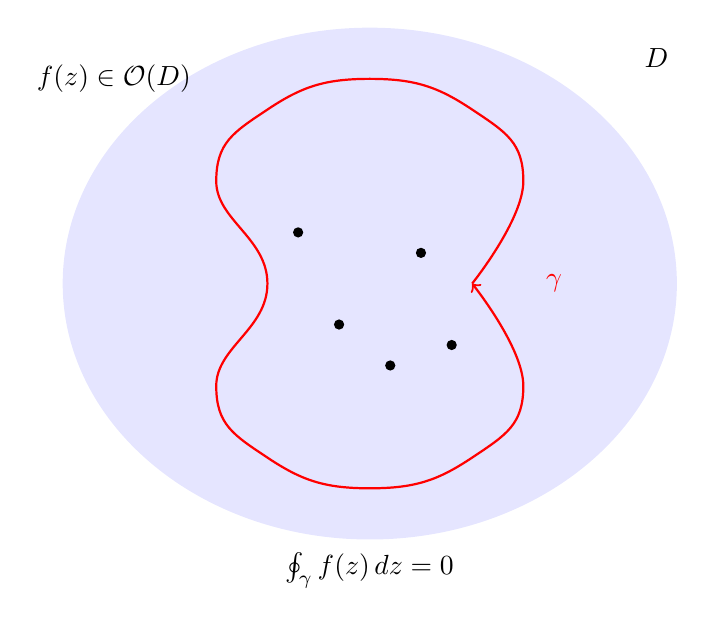
\begin{tikzpicture}[scale=1.3]
    % Draw the domain D
    \fill[blue!10] (0,0) ellipse (3 and 2.5);
    
    % Draw a simple closed curve
    \draw[thick, red, ->] plot[smooth, tension=0.8] 
      coordinates {(1,0) (1.5,1) (1,1.7) (0,2) (-1,1.7) (-1.5,1) (-1,0) (-1.5,-1) (-1,-1.7) (0,-2) (1,-1.7) (1.5,-1) (1,0)};
    
    % Label the domain and curve
    \node at (2.8,2.2) {$D$};
    \node[red] at (1.8,0) {$\gamma$};
    
    % Add a few fixed points instead of random ones
    \fill (0.5,0.3) circle (0.05);
    \fill (-0.7,0.5) circle (0.05);
    \fill (0.2,-0.8) circle (0.05);
    \fill (-0.3,-0.4) circle (0.05);
    \fill (0.8,-0.6) circle (0.05);
    
    % Add a label for the function
    \node at (-2.5,2) {$f(z) \in \mathcal{O}(D)$};
    \node at (0,-2.8) {$\oint_{\gamma} f(z) \, dz = 0$};
\end{tikzpicture}
\caption{\textit{Cauchy's Integral Theorem: The integral of a holomorphic function around any closed curve in a simply connected domain equals zero.}}
\label{fig:cauchy-integral-theorem}
\end{figure}

\subsubsection*{Proof of Cauchy's Integral Theorem}

\noindent We'll prove the theorem for a special case and then extend it. Let's assume that $f(z)$ is holomorphic in a simply connected domain $D$ and that $\gamma$ is a simple closed curve forming the boundary of a rectangle in $D$. \\

\noindent First, we'll show that the integral vanishes for a small rectangle. Let $R$ be a rectangle with vertices at $z_0$, $z_0+h$, $z_0+h+ik$, and $z_0+ik$, oriented counterclockwise.

\begin{figure}[H]
\centering
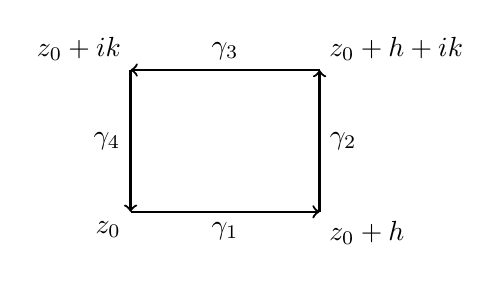
\begin{tikzpicture}[scale=1.2]
    % Draw the rectangle
    \draw[thick, ->] (0,0) -- (2,0) node[midway, below] {$\gamma_1$};
    \draw[thick, ->] (2,0) -- (2,1.5) node[midway, right] {$\gamma_2$};
    \draw[thick, ->] (2,1.5) -- (0,1.5) node[midway, above] {$\gamma_3$};
    \draw[thick, ->] (0,1.5) -- (0,0) node[midway, left] {$\gamma_4$};
    
    % Label vertices
    \node[below left] at (0,0) {$z_0$};
    \node[below right] at (2,0) {$z_0+h$};
    \node[above right] at (2,1.5) {$z_0+h+ik$};
    \node[above left] at (0,1.5) {$z_0+ik$};
\end{tikzpicture}
\caption{\textit{A rectangular contour for proving Cauchy's Integral Theorem.}}
\label{fig:cauchy-proof-rectangle}
\end{figure}

\noindent Computing the integral along each edge:
\begin{itemize}

\item Along $\gamma_1$ (from $z_0$ to $z_0+h$):
\begin{align*}
\int_{\gamma_1} f(z) \, dz &= \int_0^h f(z_0 + t) \, dt
\end{align*}

\item Along $\gamma_2$ (from $z_0+h$ to $z_0+h+ik$):
\begin{align*}
\int_{\gamma_2} f(z) \, dz &= \int_0^k f(z_0 + h + it) \, i \, dt
\end{align*}

\item Along $\gamma_3$ (from $z_0+h+ik$ to $z_0+ik$):
\begin{align*}
\int_{\gamma_3} f(z) \, dz &= \int_h^0 f(z_0 + t + ik) \, dt = -\int_0^h f(z_0 + t + ik) \, dt
\end{align*}

\item Along $\gamma_4$ (from $z_0+ik$ to $z_0$):
\begin{align*}
\int_{\gamma_4} f(z) \, dz &= \int_k^0 f(z_0 + it) \, i \, dt = -\int_0^k f(z_0 + it) \, i \, dt
\end{align*}
\end{itemize}

\noindent Adding these four integrals:
\begin{align*}
\oint_{\gamma} f(z) \, dz &= \int_0^h f(z_0 + t) \, dt + \int_0^k f(z_0 + h + it) \, i \, dt \\
&\quad - \int_0^h f(z_0 + t + ik) \, dt - \int_0^k f(z_0 + it) \, i \, dt \\
&= \int_0^h [f(z_0 + t) - f(z_0 + t + ik)] \, dt \\
&\quad + i\int_0^k [f(z_0 + h + it) - f(z_0 + it)] \, dt
\end{align*}

\noindent Now, as $h$ and $k$ become small, we can use the Mean Value Theorem and the Cauchy-Riemann equations:
\begin{align*}
f(z_0 + t + ik) - f(z_0 + t) &\approx ik \frac{\partial f}{\partial z}(z_0 + t) = ik f'(z_0 + t) \\
f(z_0 + h + it) - f(z_0 + it) &\approx h \frac{\partial f}{\partial z}(z_0 + it) = h f'(z_0 + it)
\end{align*}

\noindent Substituting into our integral:
\begin{align*}
\oint_{\gamma} f(z) \, dz &\approx -ik \int_0^h f'(z_0 + t) \, dt + ih \int_0^k f'(z_0 + it) \, dt \\
&= -ik [f(z_0 + h) - f(z_0)] + ih [f(z_0 + ik) - f(z_0)]
\end{align*}

\noindent As $h, k \to 0$, the error in our approximation approaches zero faster than the area of the rectangle, showing that:
\begin{align*}
\oint_{\gamma} f(z) \, dz = O(h^2 k + hk^2)
\end{align*}

\noindent This means that for sufficiently small rectangles, the integral approaches zero. For a general region, we can subdivide it into a grid of small rectangles. By the additivity property of line integrals, the integrals along internal edges cancel out (each is traversed twice in opposite directions), leaving only the integral around the exterior boundary. This extends the result to any simple closed curve in a simply connected domain. \\

\noindent This proof reveals an important connection: the vanishing of the integral is a direct consequence of the Cauchy-Riemann equations, which define holomorphicity. The theorem thus establishes a profound link between the differential and integral properties of complex functions.

\subsubsection*{Intuition and Significance}

\noindent To understand why Cauchy's theorem is so significant, consider the following:

\begin{enumerate}
    \item In real analysis, the integral $\int_a^b f(x) \, dx$ can be non-zero even if $f(x)$ is differentiable everywhere. For instance, $\int_0^1 1 \, dx = 1$.
    
    \item In complex analysis, Cauchy's theorem tells us that the integral of a holomorphic function around any closed loop is always zero, revealing a deep connection between complex differentiability and integration.
    
    \item Holomorphicity is a much stronger condition than real differentiability. This coupling forces the integral around closed curves to vanish.
    
    \item Geometrically, we can think of the complex line integral as measuring the ``net circulation" of the function around the curve. Cauchy's theorem tells us that holomorphic functions have zero circulation.
\end{enumerate}

\noindent Cauchy's theorem is not merely a computational tool; it reveals a deep structure in the theory of holomorphic functions that has no parallel in real analysis.

\exampleline
\begin{example}
Use Cauchy's Integral Theorem to evaluate
\[
\oint_{\gamma} \Gamma(z) \, dz
\]
where \( \gamma \) is a simple closed curve lying entirely in the right half-plane \( \Re(z) > 0 \).

\begin{solution}
We begin by recalling the integral definition of the Gamma function for \( \Re(z) > 0 \):
\[
\Gamma(z) = \int_0^\infty t^{z-1} e^{-t} \, dt
\]

\noindent To apply Cauchy's Integral Theorem, we must verify that \( \Gamma(z) \) is holomorphic on the domain \( \Re(z) > 0 \). Let \( z = x + iy \), and define
\[
\Gamma(z) = u(x,y) + i v(x,y)
\quad \text{with} \quad
t^{z-1} = t^{x-1} e^{i y \log t}
\]

Then the integrand is:
\[
t^{z-1} e^{-t} = t^{x-1} e^{-t} \left[ \cos(y \log t) + i \sin(y \log t) \right]
\]

So we have:
\[
u(x,y) = \int_0^\infty t^{x-1} e^{-t} \cos(y \log t) \, dt, \quad
v(x,y) = \int_0^\infty t^{x-1} e^{-t} \sin(y \log t) \, dt
\]

\noindent Since the integrand and its partial derivatives with respect to \( x \) and \( y \) are continuous (for \( x > 0 \)), we may differentiate under the integral sign. Then we compute:
\[
\frac{\partial u}{\partial x} = \int_0^\infty t^{x-1} e^{-t} \log t \cdot \cos(y \log t) \, dt,
\quad
\frac{\partial v}{\partial y} = \int_0^\infty t^{x-1} e^{-t} \log t \cdot \cos(y \log t) \, dt
\]

\[
\frac{\partial u}{\partial y} = -\int_0^\infty t^{x-1} e^{-t} \log t \cdot \sin(y \log t) \, dt,
\quad
\frac{\partial v}{\partial x} = \int_0^\infty t^{x-1} e^{-t} \log t \cdot \sin(y \log t) \, dt
\]

\noindent So we conclude:
\[
\frac{\partial u}{\partial x} = \frac{\partial v}{\partial y}, \quad \frac{\partial u}{\partial y} = -\frac{\partial v}{\partial x}
\]

\noindent Thus, \( \Gamma(z) \) satisfies the Cauchy-Riemann equations on the domain \( \Re(z) > 0 \), and both \( u \) and \( v \) are continuously differentiable. Therefore, \( \Gamma(z) \) is holomorphic on the right half-plane. Since \( \gamma \) lies entirely within this domain and is a simple closed curve, the hypotheses of Cauchy's Integral Theorem are satisfied. Therefore:
\[
\oint_{\gamma} \Gamma(z) \, dz = 0
\]
\end{solution}
\end{example}
\exampleline


\subsection*{Morera's Theorem} \index{Morera's Theorem}

\noindent While Cauchy's Integral Theorem tells us that holomorphic functions have vanishing integrals around closed curves, a natural question arises: Is the converse true? That is, if a function's integral vanishes around every closed curve, must the function be holomorphic? Giacinto Morera (1856-1909) answered this question affirmatively in 1886, providing an elegant characterization of holomorphicity through integration rather than differentiation. \\

\noindent \textbf{Morera's Theorem:} Let $f(z)$ be a continuous function in a simply connected domain $D$. If for every simple closed curve $\gamma$ in $D$,
\[
\oint_{\gamma} f(z) \, dz = 0
\]
then $f(z)$ is holomorphic in $D$.

\noindent This remarkable result provides an alternative path to proving holomorphicity. Rather than verifying the Cauchy-Riemann equations—which can be computationally intensive—we can sometimes more easily demonstrate that integrals vanish around closed contours. Morera's Theorem has proven particularly valuable for establishing that limits of holomorphic functions remain holomorphic, and for proving holomorphicity across boundary regions where direct verification via the Cauchy-Riemann equations might be unwieldy.

\exampleline
\begin{example}
Use Morera's Theorem to prove that the function \( f(z)=\overline{z}^2 \) is not holomorphic in any domain containing the origin.

\begin{solution}
By Morera's Theorem, if a continuous function \( f \) is holomorphic in a domain, then the integral of \( f \) over any closed contour in that domain must vanish. To show that \( f(z)=\overline{z}^2 \) is not holomorphic, it suffices to find a closed contour on which
\[
\oint_\gamma \overline{z}^2\,dz \neq 0.
\]

\noindent Consider the circle \(\gamma\) centered at \( z_0=1 \) with radius \( r=\tfrac{1}{2} \), parameterized by
\[
z(t)=1+\frac{1}{2}e^{it},\quad t\in[0,2\pi].
\]
Then,
\[
\overline{z(t)}=1+\frac{1}{2}e^{-it} \quad\text{and}\quad dz=\frac{1}{2}i\,e^{it}\,dt.
\]
Thus,
\[
\oint_\gamma \overline{z}^2\,dz = \int_0^{2\pi} \left(1+\frac{1}{2}e^{-it}\right)^2 \left(\frac{1}{2}i\,e^{it}\right)dt.
\]
Expanding the square,
\[
\left(1+\frac{1}{2}e^{-it}\right)^2 = 1+e^{-it}+\frac{1}{4}e^{-2it}.
\]
Substitute this into the integral:
\[
\oint_\gamma \overline{z}^2\,dz = \frac{i}{2}\int_0^{2\pi} \Bigl(e^{it}+1+\frac{1}{4}e^{-it}\Bigr)dt.
\]
Since
\[
\int_0^{2\pi} e^{it}\,dt=0,\quad \int_0^{2\pi}1\,dt=2\pi,\quad \int_0^{2\pi} e^{-it}\,dt=0,
\]
we obtain
\[
\oint_\gamma \overline{z}^2\,dz = \frac{i}{2}(2\pi)=\pi i\neq 0.
\]
Therefore, by Morera's Theorem, \( f(z)=\overline{z}^2 \) is not holomorphic in any domain that contains the origin.
\end{solution}
\end{example}
\exampleline


\subsection*{Cauchy's Integral Formula} \index{Cauchy's Integral Formula}

\noindent Cauchy's Integral Theorem leads to one of the most powerful tools in complex analysis: Cauchy's Integral Formula. This formula allows us to express the value of a holomorphic function at any point in terms of its values on a surrounding contour. The formula also reveals a profound connection between holomorphic functions and singularities, particularly poles, which we introduced in Chapter 7, Lecture 2 as points where a function grows unbounded. \\

\noindent \textbf{Cauchy's Integral Formula:} Let $f(z)$ be holomorphic in a simply connected domain $D$, and let $\gamma$ be a simple closed positively oriented contour in $D$. If $a$ is a point inside $\gamma$, then:
\[
f(a) = \frac{1}{2\pi i} \oint_{\gamma} \frac{f(z)}{z-a} \, dz
\]

\noindent This remarkable formula shows that if we know the values of a holomorphic function on a closed contour, we can determine its value at any point inside that contour. It's worth noting that the integrand $\frac{f(z)}{z-a}$ has a simple pole at $z = a$, but the formula works because $a$ is inside the contour. When functions have poles inside a contour, the corresponding integrals no longer vanish, which gives rise to the theory of residues we'll explore later.

\subsubsection*{Proof of Cauchy's Integral Formula}

\noindent Let \( f \) be holomorphic on a domain \( D \) and let \( \gamma \) be a positively oriented, simple closed contour contained in \( D \), with \( a \) a point inside \( \gamma \). We aim to prove that:
\[
f(a) = \frac{1}{2\pi i} \oint_\gamma \frac{f(z)}{z - a} \, dz
\]

\noindent Consider a small positively oriented circle \( \gamma_\epsilon \) of radius \( \epsilon > 0 \) centered at \( a \), fully contained within \( \gamma \) and \( D \). Define a new function
\[
g(z) = 
\begin{cases}
\frac{f(z) - f(a)}{z - a} & z \ne a \\
f'(a) & z = a
\end{cases}
\]
Since \( f \) is holomorphic, so is \( g \). Then,
\[
\frac{f(z)}{z - a} = \frac{f(a)}{z - a} + g(z)
\]

\noindent Now apply Cauchy's Theorem to the annular region between \( \gamma \) and \( \gamma_\epsilon \). The integrals over \( \gamma \) and \( \gamma_\epsilon \) cancel for \( g(z) \) since \( g \) is holomorphic on this entire region:
\[
\oint_\gamma g(z) \, dz = \oint_{\gamma_\epsilon} g(z) \, dz
\]
\[
\Rightarrow \oint_\gamma \frac{f(z)}{z - a} \, dz = f(a) \oint_\gamma \frac{1}{z - a} \, dz + \oint_\gamma g(z) \, dz
\]

\noindent By Cauchy's Theorem, \( \oint_\gamma g(z) \, dz = \oint_{\gamma_\epsilon} g(z) \, dz \), and since \( \gamma_\epsilon \) becomes arbitrarily small, this integral vanishes as \( \epsilon \to 0 \) due to the continuity of \( g \) at \( a \). Thus:
\[
\oint_\gamma \frac{f(z)}{z - a} \, dz = f(a) \oint_\gamma \frac{1}{z - a} \, dz
\]

\noindent But \( \oint_\gamma \frac{1}{z - a} \, dz = 2\pi i \) by a standard result of contour integration, so:
\[
\oint_\gamma \frac{f(z)}{z - a} \, dz = 2\pi i f(a)
\quad \Rightarrow \quad 
f(a) = \frac{1}{2\pi i} \oint_\gamma \frac{f(z)}{z - a} \, dz
\]

\noindent This completes the proof.


\begin{figure}[H]
\centering
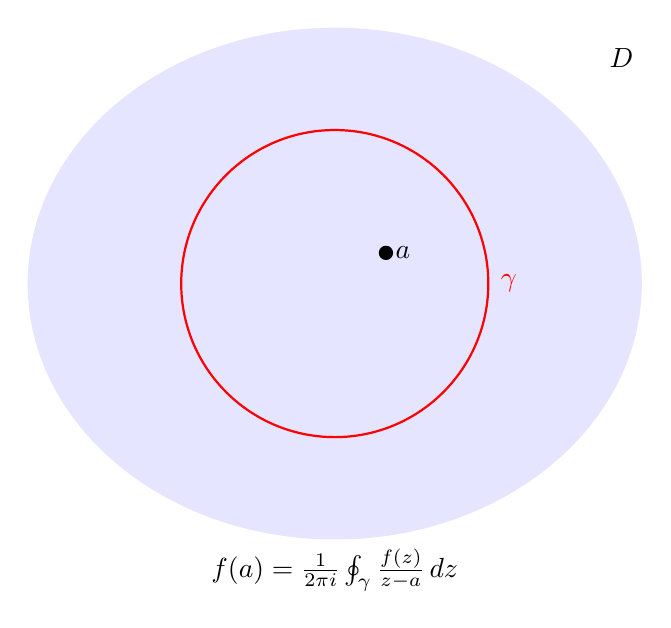
\begin{tikzpicture}[scale=1.3]
% Draw the domain D
\fill[blue!10] (0,0) ellipse (3 and 2.5);

% Draw a simple closed curve
\draw[thick, red, ->] (0,0) circle (1.5);

% Mark a point inside
\fill (0.5,0.3) circle (0.07) node[right] {$a$};

% Label the domain and curve
\node at (2.8,2.2) {$D$};
\node[red] at (1.7,0) {$\gamma$};

% Add formula
\node at (0,-2.8) {$f(a) = \frac{1}{2\pi i} \oint_{\gamma} \frac{f(z)}{z-a} \, dz$};
\end{tikzpicture}
\caption{\textit{Cauchy's Integral Formula: The value of a holomorphic function at a point is determined by its values on surrounding contours.}}
\label{fig:cauchy-integral-formula}
\end{figure}

\noindent This formula has profound implications. It shows that holomorphic functions possess a remarkable "averaging property" where their values at interior points are weighted averages of their boundary values. It also demonstrates that a holomorphic function is completely determined by its values on the boundary of its domain, reflecting the rigidity imposed by the Cauchy-Riemann equations. \\


%\subsubsection*{Related Formulas to Cauchy's Integral Formula} \index{Cauchy's Integral Formula!Key Formulas}

\noindent Cauchy's Integral Formula has many consequential results that spin off from it. Below are a collection of useful formulas and results that arise in complex analysis:

\begin{itemize}
  \item \textbf{Cauchy's Integral Formula:} 
  \[f(a) = \frac{1}{2\pi i} \oint_{\gamma} \frac{f(z)}{z-a} \, dz\]
  where $f$ is holomorphic inside and on $\gamma$, and $a$ is inside $\gamma$.
  
  \item \textbf{Cauchy's Formula for Derivatives:} 
  \[f^{(n)}(a) = \frac{n!}{2\pi i} \oint_{\gamma} \frac{f(z)}{(z-a)^{n+1}} \, dz\]
  for any non-negative integer $n$. This shows that holomorphic functions are infinitely differentiable.
  
  \item \textbf{Cauchy's Inequality:} 
  \[|f^{(n)}(a)| \leq \frac{n! \cdot M}{R^n}\]
  where $M = \max_{|z-a|=R} |f(z)|$ on the circle $|z-a| = R$. This provides bounds on the magnitudes of derivatives.
  
  \item \textbf{Integral Formula for Taylor Coefficients:} If $f(z) = \sum_{n=0}^{\infty} c_n (z-a)^n$, then:
  \[c_n = \frac{1}{2\pi i} \oint_{\gamma} \frac{f(z)}{(z-a)^{n+1}} \, dz = \frac{f^{(n)}(a)}{n!}\]
  This connects complex integration with power series representations.
\end{itemize}

\exampleline
\begin{example}
Use Cauchy's Integral Formula to evaluate $\oint_{\gamma} \frac{e^z}{z-2} \, dz$ where $\gamma$ is the circle $|z| = 3$ oriented counterclockwise.

\begin{solution}
The function $f(z) = e^z$ is holomorphic everywhere, and the point $a = 2$ lies inside the contour $\gamma$. By Cauchy's Integral Formula:

\[
f(a) = \frac{1}{2\pi i} \oint_{\gamma} \frac{f(z)}{z-a} \, dz
\]

Rearranging to solve for the integral:

\[
\oint_{\gamma} \frac{f(z)}{z-a} \, dz = 2\pi i \cdot f(a)
\]

In our case:

\[
\oint_{|z|=3} \frac{e^z}{z-2} \, dz = 2\pi i \cdot e^2 = 2\pi i e^2
\]

\noindent This demonstrates the power of Cauchy's Integral Formula: it allows us to evaluate complex integrals without direct computation, simply by knowing the value of the function at specific points.
\end{solution}
\end{example}
\exampleline
\begin{example}
Evaluate the integral
\[
\oint_{\gamma} \frac{e^{z^2}}{(z - i)^3} \, dz
\]
where \( \gamma \) is the positively oriented circle \( |z| = 2 \). What does this tell us about the value of the second derivative of \( f(z) = e^{z^2} \) at \( z = i \)?
\begin{solution}
We observe that the integrand has a third-order pole at \( z = i \), and \( f(z) = e^{z^2} \) is entire, so it's holomorphic everywhere. Since \( i \) lies inside \( \gamma \), we apply Cauchy’s Integral Formula for derivatives:

\[
f^{(n)}(a) = \frac{n!}{2\pi i} \oint_\gamma \frac{f(z)}{(z - a)^{n+1}} \, dz
\]

\noindent Here \( a = i \) and \( n = 2 \), so the exponent is \( n+1 = 3 \). Thus,
\[
\oint_{\gamma} \frac{e^{z^2}}{(z - i)^3} \, dz = 2\pi i \cdot \frac{f^{(2)}(i)}{2!}
\]

\noindent Now compute \( f^{(2)}(z) \) for \( f(z) = e^{z^2} \):
\[
f'(z) = 2z e^{z^2}, \quad f''(z) = 2e^{z^2} + 4z^2 e^{z^2} = (2 + 4z^2)e^{z^2}
\]

\noindent Then:
\[
f^{(2)}(i) = (2 + 4i^2)e^{i^2} = (2 - 4)e^{-1} = -2e^{-1}
\]

\noindent So:
\[
\oint_{\gamma} \frac{e^{z^2}}{(z - i)^3} \, dz = 2\pi i \cdot \frac{-2e^{-1}}{2} = -2\pi i \cdot \frac{e^{-1}}{1} = -2\pi i e^{-1}
\]

\noindent \textbf{Conclusion:} The value of this contour integral reveals the second derivative of \( e^{z^2} \) at \( z = i \) via pure Cauchy theory, demonstrating how the analytic structure of entire functions can be interrogated using higher-order poles.
\end{solution}
\end{example}
\exampleline

\subsection*{Laurent Series and Singular Points} \index{Laurent Series} \index{Singular Points}

\noindent While Cauchy's Integral Theorem provides powerful insights about holomorphic functions, in practical applications we frequently encounter functions with points where holomorphicity fails. What happens when we integrate around such points? This question is central to physical applications in fluid dynamics, electromagnetism, and quantum mechanics, where singularities often have physical significance representing sources, vortices, or particles. Cauchy's theorem, by itself, cannot address these cases directly, as it applies only to holomorphic functions integrated along contours in domains where they remain holomorphic. \\

\noindent To bridge this gap, we need to develop tools that characterize the behavior of functions near their singularities and provide a systematic approach to computing integrals around them. This necessity leads us to Laurent series and residue theory, which extend the scope of complex integration beyond purely holomorphic functions. When a function $f(z)$ is not holomorphic at a point $z_0$ but is holomorphic in some punctured disk $0 < |z - z_0| < R$ around this point, we call $z_0$ an isolated singularity of $f$. To understand the behavior of $f$ near such points, we need to generalize power series to include negative powers of $(z - z_0)$.

\subsubsection*{Laurent Series Expansion} \index{Laurent Series!Definition}

\noindent \textbf{Laurent Series:} Let $f(z)$ be holomorphic in an annular region $r < |z - z_0| < R$ for some $0 \leq r < R \leq \infty$. Then $f(z)$ can be represented by a series of the form:
\[
f(z) = \sum_{n=-\infty}^{\infty} a_n (z - z_0)^n = \sum_{n=0}^{\infty} a_n (z - z_0)^n + \sum_{n=1}^{\infty} \frac{a_{-n}}{(z - z_0)^n}
\]
which converges absolutely and uniformly on any compact subset of the annulus.

\noindent The coefficients $a_n$ in this expansion are given by:
\[
a_n = \frac{1}{2\pi i} \oint_\gamma \frac{f(z)}{(z - z_0)^{n+1}} \, dz
\]
where $\gamma$ is any positively oriented simple closed contour in the annulus and encircling $z_0$ once.

\begin{figure}[H]
\centering
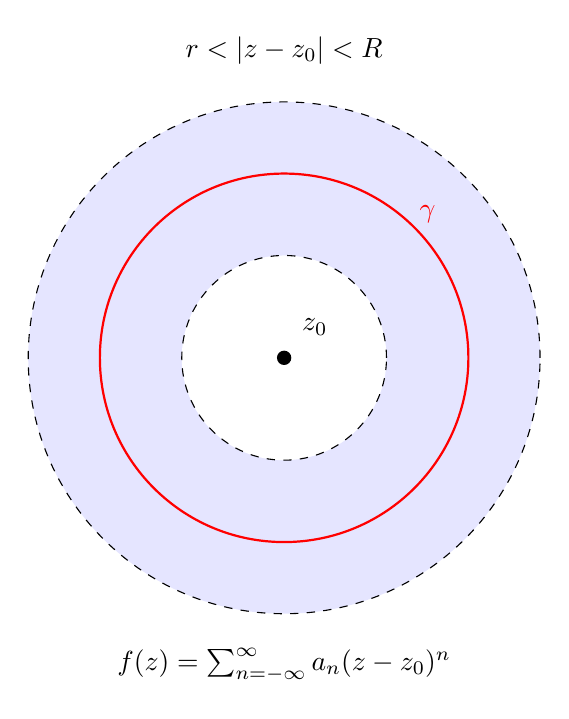
\begin{tikzpicture}[scale=1.3]
    % Draw annular region
    \fill[blue!10] (0,0) circle (2.5);
    \fill[white] (0,0) circle (1);
    
    % Draw contours
    \draw[thick, red, ->] (0,0) circle (1.8);
    \draw[dashed] (0,0) circle (1);
    \draw[dashed] (0,0) circle (2.5);
    
    % Label singularity
    \fill (0,0) circle (0.07);
    \node at (0.3,0.3) {$z_0$};
    
    % Label the annulus and curve
    \node at (0,3) {$r < |z-z_0| < R$};
    \node[red] at (1.4,1.4) {$\gamma$};
    
    % Add a label for the Laurent series
    \node at (0,-3) {$f(z) = \sum_{n=-\infty}^{\infty} a_n (z - z_0)^n$};
\end{tikzpicture}
\caption{\textit{Laurent series expansion in an annular region around an isolated singularity. The coefficients of negative powers in the expansion determine the singular behavior of the function at $z_0$.}}
\label{fig:laurent-series}
\end{figure}

\noindent The Laurent series consists of two parts:
\begin{itemize}
    \item The \textbf{analytic part} (or regular part): $\sum_{n=0}^{\infty} a_n (z - z_0)^n$, which is holomorphic at $z_0$.
    \item The \textbf{principal part}: $\sum_{n=1}^{\infty} \frac{a_{-n}}{(z - z_0)^n}$, which captures the singular behavior near $z_0$.
\end{itemize}

\noindent The existence and uniqueness of Laurent series can be established using Cauchy's Integral Formula applied to appropriately chosen contours in the annular region. The Laurent expansion provides a complete characterization of the behavior of a function near an isolated singularity.

\subsubsection*{Classification of Isolated Singularities} \index{Singularities!Classification}

\noindent Based on the Laurent series expansion, we can classify isolated singularities into three types:

\begin{enumerate}
    \item \textbf{Removable Singularity:} A point $z_0$ is a removable singularity of $f(z)$ if $a_{-n} = 0$ for all $n \geq 1$ in the Laurent expansion around $z_0$. This means the principal part vanishes, and $f$ can be defined (or redefined) at $z_0$ to be holomorphic there.
    
    \item \textbf{Pole of Order $m$:} A point $z_0$ is a pole of order $m$ if $a_{-m} \neq 0$ but $a_{-n} = 0$ for all $n > m$. Near such a point, $f(z)$ behaves like $\frac{a_{-m}}{(z - z_0)^m}$ as $z \to z_0$. We say $f$ has a simple pole at $z_0$ when $m = 1$.
    
    \item \textbf{Essential Singularity:} A point $z_0$ is an essential singularity if infinitely many coefficients $a_{-n}$ are non-zero, meaning the principal part has infinitely many terms. The behavior of $f(z)$ near an essential singularity can be extremely complicated.
\end{enumerate}

\noindent This classification is fundamental in complex analysis and provides a systematic framework for understanding the behavior of meromorphic functions—those that are holomorphic except at isolated poles.


\begin{figure}[H]
\centering
\begin{tikzpicture}[>=Latex, every node/.style={font=\small}]

  % Removable Singularity Panel (Left)
  \begin{scope}[xshift=-5cm]
    % Coordinate axes
    \draw[->] (-2,0) -- (2,0);
    \draw[->] (0,-2) -- (0,2);
    % Singularity point
    \fill[red] (0,0) circle (2pt);
    % Dashed circle showing removable behavior
    \draw[dashed] (0,0) circle (0.8cm);
  \end{scope}

  % Pole Panel (Center)
  \begin{scope}[xshift=0cm]
    % Coordinate axes
    \draw[->] (-2,0) -- (2,0);
    \draw[->] (0,-2) -- (0,2);
    % Singularity point
    \fill[red] (0,0) circle (2pt);
    % Dashed circle as a reference boundary
    \draw[dashed] (0,0) circle (0.8cm);
    % Diverging arrows illustrating blow-up
    \foreach \angle in {20, 60, 100, 140, 180, 220, 260, 300, 340} {
      \draw[->, thick] (0,0) -- (\angle:2cm);
    }
  \end{scope}

  % Essential Singularity Panel (Right)
  \begin{scope}[xshift=5cm]
    % Coordinate axes
    \draw[->] (-2,0) -- (2,0);
    \draw[->] (0,-2) -- (0,2);
    % Singularity point
    \fill[red] (0,0) circle (2pt);
    % Overlay several spirals to represent the wild oscillatory behavior:
    % An Archimedean spiral: r = 0.0318*t, with t running from 0 to 8*pi yields r_max ~0.8.
    \foreach \phi in {0,45,90} {
      \draw[domain=0:8*pi, smooth, variable=\t, samples=200, thick] 
        plot ({0.0318*\t*cos(\t r + \phi)}, {0.0318*\t*sin(\t r + \phi)});
    }
  \end{scope}

\end{tikzpicture}
\caption{Left: A removable singularity where $\lim_{z\to z_0}f(z)$ exists, as indicated by the dashed circle. Center: A pole where $|f(z)|\to\infty$, visualized by diverging arrows. Right: An essential singularity; by Picard's theorem, in any neighborhood of $z_0$, $f(z)$ assumes every complex value (with at most one exception), illustrated here by overlaid spiral curves...don't stare too long!}
\end{figure}


\exampleline
\begin{example}
Find the Laurent series expansion of $f(z) = \frac{z^2+1}{z(z-1)(z-2)}$ around $z = 0$ and classify the singularity at this point.

\begin{solution}
\noindent First, we express $f(z)$ using partial fractions:
\[
f(z) = \frac{z^2+1}{z(z-1)(z-2)} = \frac{A}{z} + \frac{B}{z-1} + \frac{C}{z-2}
\]

\noindent Multiplying both sides by $z(z-1)(z-2)$:
\[
z^2+1 = A(z-1)(z-2) + Bz(z-2) + Cz(z-1)
\]

\begin{itemize}
\item Setting $z = 0$ gives: $1 = A \cdot (-1) \cdot (-2) \Rightarrow A = \frac{1}{2}$

\item Setting $z = 1$ gives: $2 = B \cdot 1 \cdot (-1) \Rightarrow B = -2$

\item Setting $z = 2$ gives: $5 = C \cdot 2 \cdot 1 \Rightarrow C = \frac{5}{2}$
\end{itemize}
\noindent Therefore:
\[
f(z) = \frac{1/2}{z} + \frac{-2}{z-1} + \frac{5/2}{z-2} = \frac{1}{2z} - \frac{2}{z-1} + \frac{5/2}{z-2}
\]

\noindent To obtain the Laurent series around $z = 0$, we need to expand the terms with $(z-1)$ and $(z-2)$ in the denominator:
\[
\frac{1}{z-1} = -\frac{1}{1-z} = -\sum_{n=0}^{\infty} z^n \quad \text{for } |z| < 1
\]
\[
\frac{1}{z-2} = -\frac{1}{2} \cdot \frac{1}{1-\frac{z}{2}} = -\frac{1}{2}\sum_{n=0}^{\infty} \left(\frac{z}{2}\right)^n = -\frac{1}{2}\sum_{n=0}^{\infty} \frac{z^n}{2^n} \quad \text{for } |z| < 2
\]

\noindent Thus, for $0 < |z| < 1$:
\begin{align*}
f(z) &= \frac{1}{2z} - \frac{2}{z-1} + \frac{5/2}{z-2} \\
&= \frac{1}{2z} + 2\sum_{n=0}^{\infty} z^n - \frac{5}{4}\sum_{n=0}^{\infty} \frac{z^n}{2^n} \\
&= \frac{1}{2z} + 2 + 2z + 2z^2 + \cdots - \frac{5}{4} - \frac{5}{8}z - \frac{5}{16}z^2 - \cdots \\
&= \frac{1}{2z} + \left(2 - \frac{5}{4}\right) + \left(2 - \frac{5}{8}\right)z + \left(2 - \frac{5}{16}\right)z^2 + \cdots \\
&= \frac{1}{2z} + \frac{3}{4} + \frac{11}{8}z + \frac{27}{16}z^2 + \cdots
\end{align*}

\noindent Since there is only a $\frac{1}{z}$ term in the principal part (with $a_{-1} = \frac{1}{2}$), and no higher negative powers, the function has a simple pole at $z = 0$.
\end{solution}
\end{example}
\exampleline

\subsection*{Residue Theory} \index{Residue Theory}

\noindent When integrating a function with isolated singularities along a closed contour, Cauchy's Integral Theorem no longer applies directly. However, a remarkably elegant theory—residue theory—allows us to evaluate such integrals by examining the behavior of the function near each enclosed singularity.

\subsubsection*{Definition and Basic Properties of Residues} \index{Residues!Definition}

\noindent \textbf{Residue:} Given a function $f(z)$ with an isolated singularity at $z_0$ and Laurent expansion $f(z) = \sum_{n=-\infty}^{\infty} a_n (z - z_0)^n$ valid in some punctured disk around $z_0$, the residue of $f$ at $z_0$ is the coefficient $a_{-1}$ and is denoted:
\[
\text{Res}(f, z_0) = a_{-1}
\]

\noindent The fundamental importance of residues is revealed by the following theorem: \\

\noindent \textbf{Residue Theorem:} \index{Residue Theorem} Let $f(z)$ be analytic in a simply connected domain $D$ except for isolated singularities at $z_1, z_2, \ldots, z_n$. If $\gamma$ is a simple closed positively oriented contour in $D$ that doesn't pass through any of the singularities but encloses them, then:
\[
\oint_{\gamma} f(z) \, dz = 2\pi i \sum_{k=1}^{n} \text{Res}(f, z_k)
\]

\noindent This theorem reduces the evaluation of complex contour integrals to the calculation of residues at the enclosed singularities, providing a powerful computational tool.

\begin{figure}[H]
\centering
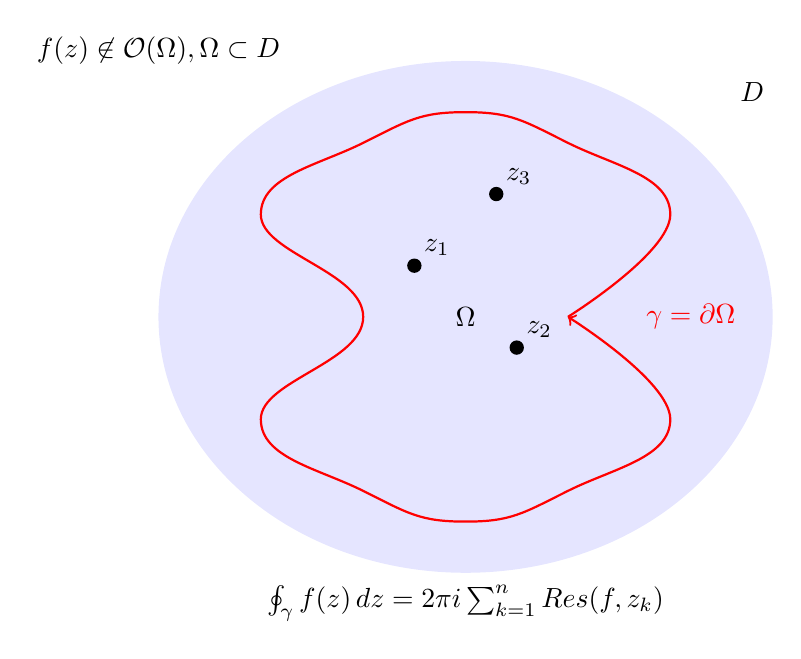
\begin{tikzpicture}[scale=1.3]
    % Draw the domain D
    \fill[blue!10] (0,0) ellipse (3 and 2.5);
    
    % Draw a simple closed curve
    \draw[thick, red, ->] plot[smooth, tension=0.8] 
      coordinates {(1,0) (2,1) (1,1.7) (0,2) (-1,1.7) (-2,1) (-1,0) (-2,-1) (-1,-1.7) (0,-2) (1,-1.7) (2,-1) (1,0)};
    
    % Mark singularities
    \fill (-0.5,0.5) circle (0.07) node[above right] {$z_1$};
    \fill (0.5,-0.3) circle (0.07) node[above right] {$z_2$};
    \fill (0.3,1.2) circle (0.07) node[above right] {$z_3$};
    
    % Label the domain and curve
    \node at (2.8,2.2) {$D$};
    \node at (-3,2.6) {$f(z) \not \in \mathcal{O}(\Omega), \Omega \subset D$};
    \node[red] at (2.2,0) {$\gamma = \partial \Omega$};
\node at (0,0) {$\Omega$};
    
    % Add formula
    \node at (0,-2.8) {$\oint_{\gamma} f(z) \, dz = 2\pi i \sum_{k=1}^{n} \text{Res}(f, z_k)$};
\end{tikzpicture}
\caption{\textit{The Residue Theorem: The integral equals $2\pi i$ times the sum of residues at enclosed singularities.}}
\label{fig:residue-theorem}
\end{figure}

\subsubsection*{Computing Residues} \index{Residues!Computation}

\noindent Several techniques exist for calculating residues, particularly for poles:

\begin{enumerate}
    \item \textbf{From Laurent Series:} If we can find the Laurent expansion of $f(z)$ around $z_0$, then $\text{Res}(f, z_0) = a_{-1}$.
    
    \item \textbf{For Simple Poles:} If $f(z) = \frac{g(z)}{h(z)}$ has a simple pole at $z_0$ (meaning $h(z_0) = 0$ but $h'(z_0) \neq 0$ and $g(z_0) \neq 0$), then:
    \[
    \text{Res}(f, z_0) = \frac{g(z_0)}{h'(z_0)}
    \]
    
    \item \textbf{For Poles of Order $m$:} If $f(z)$ has a pole of order $m$ at $z_0$, then:
    \[
    \text{Res}(f, z_0) = \frac{1}{(m-1)!} \lim_{z \to z_0} \frac{d^{m-1}}{dz^{m-1}} [(z - z_0)^m f(z)]
    \]
    
    \item \textbf{For Simple Poles with Special Form:} If $f(z) = \frac{p(z)}{q(z)}$ where $p$ and $q$ are holomorphic at $z_0$, $q(z_0) = 0$, $q'(z_0) \neq 0$, and $p(z_0) \neq 0$, then:
    \[
    \text{Res}(f, z_0) = \frac{p(z_0)}{q'(z_0)}
    \]
\end{enumerate}

\exampleline
\begin{example}
Evaluate $\oint_{\gamma} \frac{e^z}{z^2(z-1)^3} \, dz$ where $\gamma$ is the circle $|z| = 2$ oriented counterclockwise.

\begin{solution}
\noindent The function $f(z) = \frac{e^z}{z^2(z-1)^3}$ has singularities at $z = 0$ (a pole of order 2) and $z = 1$ (a pole of order 3). Both are inside the contour $\gamma: |z| = 2$. By the Residue Theorem:
\[
\oint_{\gamma} f(z) \, dz = 2\pi i [\text{Res}(f, 0) + \text{Res}(f, 1)]
\]

\noindent Let's compute each residue: \\

\noindent For $z = 0$ (pole of order 2):
\begin{align*}
\text{Res}(f, 0) &= \lim_{z \to 0} \frac{d}{dz} [z^2 f(z)] \\
&= \lim_{z \to 0} \frac{d}{dz} \left[\frac{e^z}{(z-1)^3}\right] \\
&= \lim_{z \to 0} \left[\frac{e^z}{(z-1)^3} - \frac{3e^z}{(z-1)^4}\right] \\
&= \frac{e^0}{(-1)^3} - \frac{3e^0}{(-1)^4} = -1 - 3 = -4
\end{align*}

\noindent For $z = 1$ (pole of order 3):
\begin{align*}
\text{Res}(f, 1) &= \frac{1}{2!} \lim_{z \to 1} \frac{d^2}{dz^2} [(z-1)^3 f(z)] \\
&= \frac{1}{2} \lim_{z \to 1} \frac{d^2}{dz^2} \left[\frac{e^z}{z^2}\right] 
\end{align*}

\noindent Computing the derivatives:
\begin{align*}
\frac{d}{dz} \left[e^z z^{-2}\right] &= e^z z^{-2} - 2e^z z^{-3} \\
\frac{d^2}{dz^2} \left[e^z z^{-2}\right] &= e^z z^{-2} - 2e^z z^{-3} - 2e^z z^{-3} + 6e^z z^{-4} \\
&= e^z z^{-2} - 4e^z z^{-3} + 6e^z z^{-4}
\end{align*}

\noindent Evaluating at $z = 1$:
\begin{align*}
\text{Res}(f, 1) &= \frac{1}{2}[e^1 \cdot 1^{-2} - 4e^1 \cdot 1^{-3} + 6e^1 \cdot 1^{-4}] \\
&= \frac{1}{2}[e - 4e + 6e] \\
&= \frac{3e}{2}
\end{align*}

\noindent Therefore:
\begin{align*}
\oint_{\gamma} \frac{e^z}{z^2(z-1)^3} \, dz &= 2\pi i \left[-4 + \frac{3e}{2}\right] \\
&= \pi i (3e - 8)
\end{align*}
\end{solution}
\end{example}
\exampleline
\begin{example}
Evaluate
\[
I=\oint_{\gamma} \frac{e^{1/z}}{1+z}\,dz,
\]
where \(\gamma\) is the circle \(|z|=2\) oriented counterclockwise.

\begin{solution}
\noindent The function 
\[
f(z)=\frac{e^{1/z}}{1+z}
\]
has two singularities inside \(\gamma\):
\begin{itemize}
  \item An essential singularity at \(z=0\) (from \(e^{1/z}\)),
  \item A simple pole at \(z=-1\) (since \(1+z=0\)).
\end{itemize}

\noindent By the Residue Theorem:
\[
I=2\pi i\left[\operatorname{Res}(f,0)+\operatorname{Res}(f,-1)\right].
\]

\noindent For the residue at \(z=-1\), which is a simple pole:
\begin{align*}
\operatorname{Res}(f,-1) &= \lim_{z\to -1}(z+1)f(z) \\
&= \lim_{z\to -1} \frac{(z+1) \cdot e^{1/z}}{1+z} \\
&= \lim_{z\to -1} e^{1/z} \\
&= e^{-1}
\end{align*}

\noindent For the residue at \(z=0\), which is an essential singularity, we need to find the coefficient of \(z^{-1}\) in the Laurent series expansion. We expand each factor:
\[
e^{1/z}=\sum_{n=0}^{\infty}\frac{1}{n!}\,\frac{1}{z^n}
\]
and 
\[
\frac{1}{1+z}=\sum_{m=0}^{\infty}(-1)^m z^m \quad \text{for } |z| < 1
\]

\noindent Multiplying these series:
\[
\frac{e^{1/z}}{1+z}=\sum_{n=0}^{\infty}\sum_{m=0}^{\infty}\frac{(-1)^m}{n!}\,z^{m-n}
\]

\noindent The \(z^{-1}\) term appears when \(m-n=-1\), or \(m=n-1\). Therefore:
\begin{align*}
\operatorname{Res}(f,0) &= \sum_{n=1}^{\infty}\frac{(-1)^{n-1}}{n!} \\
&= -\sum_{n=1}^{\infty}\frac{(-1)^{n}}{n!} \\
&= -\left(\sum_{n=0}^{\infty}\frac{(-1)^{n}}{n!} - 1\right) \\
&= -\left(e^{-1} - 1\right) \\
&= 1-e^{-1}
\end{align*}

\noindent Adding the residues:
\begin{align*}
\operatorname{Res}(f,0)+\operatorname{Res}(f,-1) &= (1-e^{-1})+e^{-1} \\
&= 1
\end{align*}

\noindent Therefore, by the Residue Theorem:
\[
I=2\pi i \cdot 1 = 2\pi i
\]
\end{solution}
\end{example}
\exampleline

\subsection*{Applications to Real Definite Integrals} \index{Residue Theory!Real Integrals}

\noindent One of the most powerful applications of residue theory is the evaluation of real definite integrals that would be difficult or impossible to compute using elementary calculus techniques. The strategy involves transforming a real integral into a complex contour integral, applying the residue theorem, and then extracting the value of the original integral. \\

\noindent This approach is particularly effective for three classes of integrals:

\begin{enumerate}
    \item \textbf{Rational Functions on the Entire Real Line:} Integrals of the form $\int_{-\infty}^{\infty} \frac{P(x)}{Q(x)} \, dx$ where $P$ and $Q$ are polynomials with $\deg(P) < \deg(Q)$.
    
    \item \textbf{Trigonometric Integrals:} Integrals of the form $\int_{0}^{2\pi} R(\cos \theta, \sin \theta) \, d\theta$ where $R$ is a rational function.
    
    \item \textbf{Integrals with Exponential Factors:} Integrals like $\int_{-\infty}^{\infty} \frac{e^{iax}}{P(x)} \, dx$ or $\int_{-\infty}^{\infty} \frac{\cos(ax)}{P(x)} \, dx$.
\end{enumerate}

\subsubsection*{Key Transformations and Techniques}

\noindent Several transformations and identities facilitate the conversion between real and complex integrals:

\begin{itemize}
    \item \textbf{Substitution $z = e^{i\theta}$:} This transforms trigonometric functions:
    \begin{align*}
        \cos\theta &= \frac{z + z^{-1}}{2} \\
        \sin\theta &= \frac{z - z^{-1}}{2i} \\
        d\theta &= \frac{dz}{iz}
    \end{align*}
    With this substitution, $\int_{0}^{2\pi} f(\cos\theta, \sin\theta) \, d\theta$ becomes $\oint_{|z|=1} f\left(\frac{z + z^{-1}}{2}, \frac{z - z^{-1}}{2i}\right) \frac{dz}{iz}$.
    
    \item \textbf{Contour Selection:} For integrals over $(-\infty, \infty)$, we often use a semicircular contour in the upper half-plane, consisting of the real axis from $-R$ to $R$ and a semicircle $\Gamma_R$ of radius $R$ in the upper half-plane.
    
    \item \textbf{Jordan's Lemma:} For integrals of the form $\int_{-\infty}^{\infty} f(x)e^{iax} \, dx$ with $a > 0$, the contribution from the upper semicircular contour $\Gamma_R$ vanishes as $R \to \infty$ if $f(z) \to 0$ as $|z| \to \infty$ in the upper half-plane.
    
    \item \textbf{Evaluation of Real Integrals Using Complex Methods:}
    \begin{align*}
        \int_{-\infty}^{\infty} \frac{P(x)}{Q(x)} \, dx &= 2\pi i \sum_{\text{Im}(z_k) > 0} \text{Res}\left(\frac{P(z)}{Q(z)}, z_k\right) \\
        \int_{0}^{\infty} f(x) \, dx &= \int_{0}^{\infty} f(x) \, dx + i \int_{0}^{\infty} f(ix) \, dx \\
        &= 2\pi i \sum_{\text{Re}(z_k) > 0, \text{Im}(z_k) > 0} \text{Res}(f(z), z_k)
    \end{align*}
    where $z_k$ are the poles in the specified regions.
\end{itemize}

\subsubsection*{Important Relations for Trigonometric Integrals}

\noindent When dealing with trigonometric integrals, these identities are particularly useful:
\begin{align*}
    \cos^2\theta &= \frac{1 + \cos 2\theta}{2} = \frac{1}{2} + \frac{z^2 + z^{-2}}{4} \\
    \sin^2\theta &= \frac{1 - \cos 2\theta}{2} = \frac{1}{2} - \frac{z^2 + z^{-2}}{4} \\
    \cos^n\theta &= \frac{1}{2^n}\sum_{k=0}^{n} \binom{n}{k} \cos((n-2k)\theta) \\
    \sin^n\theta &= \frac{1}{2^n}\sum_{k=0}^{\lfloor n/2 \rfloor} (-1)^k \binom{n}{k} \sin((n-2k)\theta)
\end{align*}

\noindent After substituting $z = e^{i\theta}$, a rational function of trigonometric functions transforms into a rational function of $z$, allowing us to apply residue theory effectively.

\exampleline
\begin{example}
Evaluate the challenging trigonometric integral:
\[
I = \int_{0}^{2\pi} \frac{d\theta}{(2 + \cos\theta)^2}
\]

\begin{solution}
\noindent This integral appears formidable using standard techniques. We'll solve it using residue theory with the substitution $z = e^{i\theta}$.

\noindent First, let's express $\cos\theta$ in terms of $z$:
\[
\cos\theta = \frac{z + z^{-1}}{2}
\]
and note that:
\[
d\theta = \frac{dz}{iz}
\]

\noindent The integral becomes:
\begin{align*}
I &= \int_{0}^{2\pi} \frac{d\theta}{(2 + \cos\theta)^2} \\
&= \oint_{|z|=1} \frac{1}{\left(2 + \frac{z + z^{-1}}{2}\right)^2} \cdot \frac{dz}{iz} \\
&= \oint_{|z|=1} \frac{1}{\left(\frac{4z + z^2 + 1}{2z}\right)^2} \cdot \frac{dz}{iz} \\
&= \frac{1}{i} \oint_{|z|=1} \frac{4z}{\left(z^2 + 4z + 1\right)^2} \, dz
\end{align*}

\noindent We need to find the poles of the integrand by solving $z^2 + 4z + 1 = 0$:
\begin{align*}
z &= \frac{-4 \pm \sqrt{16 - 4}}{2} \\
&= \frac{-4 \pm \sqrt{12}}{2} \\
&= -2 \pm \sqrt{3}
\end{align*}

\noindent This gives $z_1 = -2 + \sqrt{3} \approx -0.268$ and $z_2 = -2 - \sqrt{3} \approx -3.732$. Since $|z_1| < 1$ and $|z_2| > 1$, only $z_1$ lies inside the unit circle. The pole at $z_1$ is of order 2, so we use the formula for a second-order pole:
\begin{align*}
\text{Res}(f, z_1) &= \lim_{z \to z_1} \frac{d}{dz}\left[(z - z_1)^2 \cdot \frac{4z}{\left(z^2 + 4z + 1\right)^2}\right] \\
&= \lim_{z \to z_1} \frac{d}{dz}\left[\frac{4z}{(z - z_1)^2 \cdot (z - z_2)^2} \cdot (z - z_1)^2\right] \\
&= \lim_{z \to z_1} \frac{d}{dz}\left[\frac{4z}{(z - z_2)^2}\right]
\end{align*}

\noindent Computing the derivative:
\begin{align*}
\frac{d}{dz}\left[\frac{4z}{(z - z_2)^2}\right] &= \frac{4 \cdot (z - z_2)^2 - 4z \cdot 2(z - z_2)}{(z - z_2)^4} \\
&= \frac{4(z - z_2)^2 - 8z(z - z_2)}{(z - z_2)^4} \\
&= \frac{-4(z + z_2)}{(z - z_2)^3}
\end{align*}

\noindent Evaluating at $z = z_1$:
\begin{align*}
\text{Res}(f, z_1) &= \frac{-4(z_1 + z_2)}{(z_1 - z_2)^3} \\
&= \frac{-4(-2 + \sqrt{3} - 2 - \sqrt{3})}{((-2 + \sqrt{3}) - (-2 - \sqrt{3}))^3} \\
&= \frac{2\sqrt{3}}{9}
\end{align*}

\noindent By the Residue Theorem:
\begin{align*}
I &= \frac{1}{i} \cdot 2\pi i \cdot \text{Res}(f, z_1) \\
&= \frac{4\pi\sqrt{3}}{9}
\end{align*}

\noindent Therefore:
\[
\int_{0}^{2\pi} \frac{d\theta}{(2 + \cos\theta)^2} = \frac{4\pi\sqrt{3}}{9}
\]

\noindent This example demonstrates the power of residue theory in evaluating trigonometric integrals that would be extremely challenging using elementary techniques.
\end{solution}
\end{example}
\exampleline


\newpage

\formsdefs{}

\subsection*{Important Vocabulary}
\begin{itemize}
    \item \textbf{Complex Number:} A number of the form $z = a + bi$ where $a$ and $b$ are real numbers and $i$ is the imaginary unit satisfying $i^2 = -1$.
    
    \item \textbf{Real Part:} For $z = a + bi$, the real part $\Re(z) = a$.
    
    \item \textbf{Imaginary Part:} For $z = a + bi$, the imaginary part $\Im(z) = b$.
    
    \item \textbf{Complex Conjugate:} For $z = a + bi$, the complex conjugate $\overline{z} = a - bi$.
    
    \item \textbf{Modulus/Absolute Value:} For $z = a + bi$, the modulus $|z| = \sqrt{a^2 + b^2}$.
    
    \item \textbf{Argument:} The angle $\theta = \arg(z)$ such that $z = |z|e^{i\theta}$.
    
    \item \textbf{Holomorphic Function:} A complex function that is complex differentiable in a neighborhood of every point in its domain.
    
    \item \textbf{Analytic Function:} A function that can be represented by a convergent power series in a neighborhood of each point in its domain.
    
    \item \textbf{Singularity:} A point where a function is not holomorphic.
    
    \item \textbf{Pole:} A singularity where a function becomes unbounded.
    
    \item \textbf{Essential Singularity:} A non-removable singularity that is not a pole.
    
    \item \textbf{Residue:} The coefficient of $(z-z_0)^{-1}$ in the Laurent series expansion of a function around $z_0$.
    
    \item \textbf{Branch Cut:} A curve in the complex plane across which a multi-valued function is discontinuous.
    
    \item \textbf{Conformal Mapping:} A transformation that locally preserves angles.
    
    \item \textbf{Simply Connected Domain:} A domain where every simple closed curve can be continuously shrunk to a point within the domain.
\end{itemize}

\subsection*{Key Formulas}
\begin{multicols}{2}

\paragraph{Basic Operations:}
\[
(a + bi) + (c + di) = (a + c) + (b + d)i
\]
\[
(a + bi)(c + di) = (ac - bd) + (ad + bc)i
\]
\[
\frac{a + bi}{c + di} = \frac{(a + bi)(c - di)}{(c + di)(c - di)} = \frac{ac + bd}{c^2 + d^2} + \frac{bc - ad}{c^2 + d^2}i
\]

\paragraph{Complex Conjugate:}
\[
\overline{z} = \overline{a + bi} = a - bi
\]
\[
\overline{z_1 + z_2} = \overline{z_1} + \overline{z_2}
\]
\[
\overline{z_1 \cdot z_2} = \overline{z_1} \cdot \overline{z_2}
\]
\[
z \cdot \overline{z} = |z|^2 = a^2 + b^2
\]

\paragraph{Modulus/Absolute Value:}
\[
|z| = \sqrt{a^2 + b^2} = \sqrt{z\overline{z}}
\]
\[
|z_1 \cdot z_2| = |z_1| \cdot |z_2|
\]
\[
\left|\frac{z_1}{z_2}\right| = \frac{|z_1|}{|z_2|}
\]

\paragraph{Polar Form:}
\[
z = a + bi = r(\cos\theta + i\sin\theta) = re^{i\theta}
\]
\[
r = |z| = \sqrt{a^2 + b^2}
\]
\[
\theta = \arg(z) = \arctan\left(\frac{b}{a}\right)
\]

\paragraph{Euler's Formula:}
\[
e^{i\theta} = \cos\theta + i\sin\theta
\]
\[
e^{z} = e^{x}(\cos y + i\sin y) \quad \text{for } z = x + iy
\]

\paragraph{De Moivre's Theorem:}
\[
(re^{i\theta})^n = r^n e^{in\theta} = r^n(\cos(n\theta) + i\sin(n\theta))
\]

\paragraph{$n$th Roots of Complex Numbers:}
\[
w_k = \sqrt[n]{r}e^{i(\theta + 2\pi k)/n}, \quad k = 0,1,\ldots,n-1
\]

\paragraph{Roots of Unity:}
\[
\zeta_k = e^{2\pi i k/n}, \quad k = 0,1,\ldots,n-1
\]

\paragraph{Exponential Function:}
\[
e^{z} = \sum_{n=0}^{\infty} \frac{z^n}{n!}
\]

\paragraph{Trigonometric Functions:}
\[
\sin(z) = \frac{e^{iz} - e^{-iz}}{2i}
\]
\[
\cos(z) = \frac{e^{iz} + e^{-iz}}{2}
\]

\paragraph{Complex Logarithm:}
\[
\ln(z) = \ln|z| + i \arg(z)
\]
\[
\Log(z) = \ln|z| + i\,\Arg(z) \quad \text{(principal branch)}
\]

\paragraph{Complex Derivatives:}
\[
f'(z_0) = \lim_{\Delta z \to 0} \frac{f(z_0 + \Delta z) - f(z_0)}{\Delta z}
\]

\paragraph{Cauchy-Riemann Equations:}
For $f(z) = u(x,y) + iv(x,y)$, where $z = x + iy$:
\[
\frac{\partial u}{\partial x} = \frac{\partial v}{\partial y}, \quad \frac{\partial u}{\partial y} = -\frac{\partial v}{\partial x}
\]

\paragraph{Polar Cauchy-Riemann Equations:}
\[
\frac{\partial u}{\partial r} = \frac{1}{r}\frac{\partial v}{\partial \theta}, \quad \frac{\partial v}{\partial r} = -\frac{1}{r}\frac{\partial u}{\partial \theta}
\]

\paragraph{Rules of Differentiation:}
\[
(f+g)'(z) = f'(z)+g'(z)
\]
\[
(f\cdot g)'(z) = f'(z)g(z)+f(z)g'(z)
\]
\[
\left(\frac{f}{g}\right)'(z) = \frac{f'(z)g(z)-f(z)g'(z)}{[g(z)]^2}
\]
\[
(f\circ g)'(z) = f'(g(z))g'(z)
\]

\paragraph{Power Series:}
\[
f(z) = \sum_{n=0}^{\infty} a_n (z - z_0)^n
\]
\[
a_n = \frac{f^{(n)}(z_0)}{n!}
\]

\paragraph{Complex Line Integral:}
\[
\int_{\gamma} f(z) \, dz = \int_a^b f(\gamma(t)) \, \gamma'(t) \, dt
\]

\paragraph{Complex Line Integral in Component Form:}
\[
\int_{\gamma} f(z) \, dz = \int_a^b [u \cdot x' - v \cdot y' + i(u \cdot y' + v \cdot x')] \, dt
\]

\paragraph{ML Inequality:}
\[
\left| \int_{\gamma} f(z) \, dz \right| \leq L(\gamma) \cdot \max_{z \in \gamma} |f(z)|
\]

\paragraph{Fundamental Theorem for Line Integrals:}
\[
\int_{\gamma} f(z) \, dz = F(z_2) - F(z_1)
\]
where $F'(z) = f(z)$ and $\gamma$ is a path from $z_1$ to $z_2$.

\paragraph{Cauchy's Integral Theorem:}
\[
\oint_{\gamma} f(z) \, dz = 0
\]
for $f$ holomorphic within and on a simple closed contour $\gamma$.

\paragraph{Cauchy's Integral Formula:}
\[
f(a) = \frac{1}{2\pi i} \oint_{\gamma} \frac{f(z)}{z-a} \, dz
\]
where $\gamma$ is a simple closed contour containing $a$.

\paragraph{Cauchy's Formula for Derivatives:}
\[
f^{(n)}(a) = \frac{n!}{2\pi i} \oint_{\gamma} \frac{f(z)}{(z-a)^{n+1}} \, dz
\]

\paragraph{Cauchy's Inequality:}
\[
|f^{(n)}(a)| \leq \frac{n! \cdot M}{R^n}
\]
where $M = \max_{|z-a|=R} |f(z)|$.

\paragraph{Laurent Series:}
\begin{align*}
f(z) &= \sum_{n=-\infty}^{\infty} a_n (z - z_0)^n \\
&= \sum_{n=0}^{\infty} a_n (z - z_0)^n + \sum_{n=1}^{\infty} \frac{a_{-n}}{(z - z_0)^n}
\end{align*}

\paragraph{Laurent Series Coefficients:}
\[
a_n = \frac{1}{2\pi i} \oint_{\gamma} \frac{f(z)}{(z - z_0)^{n+1}} \, dz
\]

\paragraph{Residue Theorem:}
\[
\oint_{\gamma} f(z) \, dz = 2\pi i \sum_{k=1}^{n} \text{Res}(f, z_k)
\]
where $z_k$ are the poles of $f$ inside $\gamma$.

\paragraph{Residue Computation (Simple Pole):}
\[
\text{Res}(f, z_0) = \lim_{z \to z_0} (z - z_0)f(z)
\]

\paragraph{Residue for Simple Pole with Special Form:}
\[
\text{Res}(f, z_0) = \frac{p(z_0)}{q'(z_0)}
\]
for $f(z) = \frac{p(z)}{q(z)}$ where $q(z_0) = 0$ and $q'(z_0) \neq 0$

\paragraph{Residue Computation (Pole of Order $m$):}
\[
\text{Res}(f, z_0) = \frac{1}{(m-1)!} \lim_{z \to z_0} \frac{d^{m-1}}{dz^{m-1}} [(z - z_0)^m f(z)]
\]

\paragraph{Winding Number:}
\[
n(\gamma, a) = \frac{1}{2\pi i} \oint_{\gamma} \frac{dz}{z-a}
\]

\paragraph{Integration Along Unit Circle:}
\[
\oint_{|z|=1} z^n dz = \begin{cases}
0 & \text{if } n \neq -1 \\
2\pi i & \text{if } n = -1
\end{cases}
\]

\end{multicols}

\newpage


\practice{}

\begin{multicols}{2}

\begin{enumerate}
\item Compute the modulus and complex conjugate of the number \( 3-4i \). Verify that 
\[
(3-4i)(3+4i)=|3-4i|^2.
\]
%
\item Given \( z_1 = 2+3i \) and \( z_2 = -1+4i \), find:
  \begin{enumerate}
    \item \( z_1+z_2 \)
    \item \( z_1-z_2 \)
    \item \( z_1z_2 \)
    \item \( \dfrac{z_1}{z_2} \)
  \end{enumerate}
Express all answers in the form \( a+bi \).

\item Express the complex number \( -1-i \) in polar form by determining its modulus and argument.

\item Use Euler's formula to show that 
\[
\cos\theta+i\sin\theta=e^{i\theta},
\]
and compare the first few terms of the Taylor series on both sides to verify the equality.

\item Use De Moivre's theorem to compute 
\[
\left(\frac{\sqrt{2}}{2}+i\frac{\sqrt{2}}{2}\right)^5,
\]
and then express your answer in rectangular form.

\item Find all cube roots of \( 8i \). Express your answers both in polar form and in the form \( a+bi \).

\item Solve the equation 
\[
z^2+4=0
\]
using polar representation, and write the solutions in \( a+bi \) form.

\item Describe the geometric transformation on the complex plane corresponding to multiplication by \(-i\). Choose a nonzero complex number to illustrate how its position changes.

\item Find all complex numbers \( z \) satisfying 
\[
|z-(1+2i)|=3.
\]
Describe the geometric locus of these points in the Argand plane.

\item Determine all the 5th roots of unity, and sketch their approximate positions on the complex plane.

\item Verify that for \( z=5-2i \), the product \( z\overline{z} \) equals \( |z|^2 \) by direct computation.

\item Determine the locus of points \( z \) in the complex plane that satisfy 
\[
|z-2|=|z+2|.
\]
Explain the geometric significance of this locus.

\item Factorize the polynomial 
\[
z^3-8
\]
completely over \(\mathbb{C}\), and find all its roots.

\item Solve the equation 
\[
z^4+16=0
\]
by expressing the solutions in polar form and then converting them to rectangular form.

\item Solve the quadratic equation 
\[
z^2+(3-2i)z+(5-i)=0
\]
using the quadratic formula for complex coefficients, and express the solutions in the form \( a+bi \).


\item
For \( f(z)=z^2 \) with \( z=x+iy \), write \( f(z)=u(x,y)+iv(x,y) \) by expanding \((x+iy)^2\). Identify \( u(x,y) \) and \( v(x,y) \). Then, show that if \( z \) lies on the real axis, its image under \( f \) is also real.

\item
Express \( f(z)=\frac{1}{z} \) in terms of \( x \) and \( y \) for \( z=x+iy \) (by rationalizing the denominator) and identify the real function \( u(x,y) \) and the imaginary function \( v(x,y) \). Also, state the set of points where \( f(z) \) is undefined.

\item
For \( f(z)=e^z \), write \( f(z)=e^x(\cos y + i\sin y) \) when \( z=x+iy \). Describe the image of the vertical line \( x=0 \) (i.e. \( z=iy \)) in the \( w \)-plane.

\item
Determine the natural domain of \( f(z)=\ln(z) \) in the complex plane and explain how and why a branch cut (e.g. along the negative real axis) is introduced to obtain a single-valued principal branch.

\item
Starting from the definition 
\[
\sin(z)=\frac{e^{iz}-e^{-iz}}{2i},
\]
derive the form 
\[
\sin(z)=\sin x \cosh y + i\cos x \sinh y,
\]
for \( z=x+iy \).

\item
Solve \( e^{z}=-2 \) for \( z \) by writing \( z=x+iy \) and expressing the answer in the form \( x+iy \). List all solutions.

\item
Let \( f(z)=z^3 \). Show that if \( z \) lies on the unit circle (i.e. \( |z|=1 \)), then \( f(z) \) also lies on the unit circle and its argument is tripled. Verify this with \( z=e^{i\pi/3} \).

\item
Consider \( f(z)=\frac{z^2+1}{z-i} \). Determine its domain in \( \mathbb{C} \) and identify any singularities. Specify the type and order (if applicable) of each singularity.

\item
Define \( f(z)=\sqrt{z} \) using the principal branch with a branch cut along the negative real axis. Compute \( f(4e^{i\pi}) \) and express your answer in the form \( a+bi \).

\item 
For \( f(z)=\ln(z) \), compute all values of \( \ln(-1-i) \) in terms of its modulus and argument. Then, specify the principal value using the conventional range \( (-\pi,\pi] \) for the argument.

\item
Determine the image of the horizontal line \( y=1 \) (i.e. \( z=x+i \)) under the mapping \( f(z)=e^z \). Describe the geometric nature of the resulting curve in the \( w \)-plane.

\item
Solve the equation \( \cos(z)=0 \) for all \( z\in\mathbb{C} \). (Hint: Use the definition \( \cos(z)=\frac{e^{iz}+e^{-iz}}{2} \) and set up an exponential equation.)

\item
For \( f(z)=z+\frac{1}{z} \), determine the condition(s) on \( z \) so that \( f(z) \) is a real number. Express your answer in terms of the real and imaginary parts of \( z \).

\item 
Consider \( f(z)=\frac{z-1}{z+1} \). Prove that \( f \) maps the imaginary axis (i.e. \( z=iy \) with \( y\in\mathbb{R} \)) into the unit circle.

\item
Let \( f(z)=e^{z^2} \). Express \( f(z) \) in terms of \( x \) and \( y \) for \( z=x+iy \). 

  \item Evaluate the following limits:
    \begin{enumerate}
      \item \( \displaystyle \lim_{z \to 0} z^3 \).
      \item \( \displaystyle \lim_{z \to 0} \frac{\sin z}{z} \).
      \item \( \displaystyle \lim_{z \to 0} \frac{e^z - 1}{z} \).
      \item \( \displaystyle \lim_{z \to 0} \frac{1 - \cos z}{z^2} \).
    \end{enumerate}

  \item Using the Taylor series expansion for \(\sin z\), evaluate
    \[
    \lim_{z \to 0} \frac{\sin z - z}{z^3}\,.
    \]

  \item Compute
    \[
    \lim_{z \to 1+i} \frac{z^3 - (1+i)^3}{\,z - (1+i)}\,.
    \]
    (Hint: Factor the numerator or interpret the limit as the derivative of \(z^3\) at \(z=1+i\).)

  \item Prove, using the epsilon–delta definition, that for any integer \(n \ge 1\)
    \[
    \lim_{z\to 0} z^n = 0\,.
    \]

\item Using polar form, prove that \( \displaystyle \lim_{r\to 0} r\,e^{2i\theta}=0 \) (the limit is independent of \(\theta\)).

\item Let \( f(z)=\frac{z^2-\overline{z}^2}{\,z-\overline{z}} \) (with \(z\notin\mathbb{R}\)). Evaluate \( \displaystyle \lim_{z\to 2+i} f(z) \).

  \item Show that by writing \(z = re^{i\theta}\)
    \[
    \lim_{r \to 0} r\,e^{2i\theta} = 0\,,
    \]
    and explain why this limit does not depend on the angle \(\theta\).

  \item Prove that
    \[
    \lim_{z\to 0} \frac{\overline{z}}{z}
    \]
    does not exist by showing that the value depends on the direction (i.e. on \(\theta\)) along which \(z\) approaches \(0\).

  \item
    \begin{enumerate}
      \item Evaluate \( \displaystyle \lim_{|z|\to\infty} \frac{1}{z}\) in the extended complex plane.
      \item Determine whether the limit
        \[
        \lim_{z\to\infty} \frac{z}{|z|}
        \]
        exists; justify your answer.
    \end{enumerate}

  \item Evaluate
    \[
    \lim_{z\to 0}\frac{e^z - e^{\overline{z}}}{\,z - \overline{z}}\,.
    \]
    (Hint: Express \(z = x+iy\) so that \(z-\overline{z}=2iy\), then simplify using the series for \(e^z\).)

  \item  Write down the epsilon–delta definition of the limit
    \[
    \lim_{z\to z_0} f(z) = L
    \]
    for a complex function \(f\), and explain why path independence (i.e. the fact that the limit must be the same along every approach to \(z_0\)) is crucial in \(\mathbb{C}\).

  \item Describe the extended complex plane \(\hat{\mathbb{C}} = \mathbb{C} \cup \{\infty\}\) and, using the epsilon–delta idea adapted for infinity, prove that
    \[
    \lim_{z\to 0}\frac{1}{z} = \infty\,.
    \]


  \item Using the definition of the derivative, compute
  \[
  f'(z) \quad \text{for} \quad f(z)=z^2.
  \]

  \item Using the limit definition, show that
  \[
  (e^z)'=e^z.
  \]

  \item Using the limit definition (and the power series of the logarithm), prove that on its principal branch
  \[
  (\Log z)'=\frac{1}{z}\quad \text{for } z\not\in(-\infty,0].
  \]

  \item Compute the derivative of
  \[
  f(z)=\sin z
  \]
  by directly applying the definition.

  \item Use the limit definition to differentiate
  \[
  f(z)=\frac{1}{z},
  \]
  for \(z\neq 0\).

  \item Show that the function
  \[
  f(z)=|z|^2
  \]
  is not complex differentiable at any point \(z\neq 0\) (by considering different paths of approach).

  \item Prove that the function
  \[
  f(z)=\Re(z)
  \]
  is nowhere differentiable in \(\mathbb{C}\).

  \item Write \(f(z)=z^3\) in Cartesian form and verify that its real and imaginary components satisfy the Cauchy-Riemann equations.

  \item Check that the function
  \[
  f(z)=\overline{z}
  \]
  fails the Cauchy-Riemann equations, and conclude that it is not holomorphic.

  \item Prove (outline a proof) the chain rule for complex functions: that if \(g\) is holomorphic at \(z_0\) and \(f\) is holomorphic at \(g(z_0)\), then
  \[
  (f\circ g)'(z_0)=f'(g(z_0))\cdot g'(z_0).
  \]

  \item Differentiate the functions
\begin{enumerate}
 \item  \(
  f(z)=z^2\cdot e^z
  \)

 \item  \(
  f(z)=\sin\bigl(e^z\bigr).
  \)

 \item  \(
  f(z)=z^3+2z^2-3z+1
  \)
\end{enumerate}

  \item For the function defined on the principal branch by
  \[
  f(z)=z^{3/2},
  \]
  express \(z\) in polar form and compute \(f'(z)\).

  \item Prove that if \(f'(z)=0\) for all \(z\) in a connected domain, then \(f\) is constant. (Hint: Use the uniqueness of antiderivatives.)

\item Express the function 
\[
f(z)=z^2
\]
in polar coordinates. Derive the polar form of the Cauchy–Riemann equations
\[
u_r=\frac{1}{r}\,v_\theta \quad \text{and} \quad v_r=-\frac{1}{r}\,u_\theta,
\]
and verify that these hold for \(f(z)\).

  \item
    Show that 
    \[
    u(x,y)=\frac{1}{2}\ln(x^2+y^2)
    \]
    is harmonic on \(\mathbb{R}^2\setminus\{(0,0)\}\); that is, verify that 
    \[
    u_{xx}(x,y)+u_{yy}(x,y)=0
    \]
    for all \((x,y)\neq(0,0)\).

  \item
    Prove that 
    \[
    u(x,y)=e^x\cos y
    \]
    is a harmonic function on \(\mathbb{R}^2\); in other words, show that it satisfies Laplace’s equation
    \[
    u_{xx}+u_{yy}=0.
    \]

  \item
    Verify that the real part of \(z^3\), namely 
    \[
    u(x,y)=x^3-3xy^2,
    \]
    is harmonic in \(\mathbb{R}^2\) by showing that 
    \[
    u_{xx}(x,y)+u_{yy}(x,y)=0.
    \]

  \item
    Find the power series expansion of 
    \[
    f(z)=\frac{1}{1-z}
    \]
    about \(z=0\) and determine its radius of convergence.

  \item
    Expand 
    \[
    f(z)=\Log(1+z)
    \]
    in a Taylor series around \(z=0\) (using the principal branch) and state its radius of convergence.


  \item Let \(\gamma\) be the straight line segment from \(z=1+0i\) to \(z=1+2i\). Compute the integral
  \[
  \int_{\gamma} dz.
  \]
 
  
  \item Let \(\gamma\) be the straight line from \(z=0\) to \(z=1+i\). Compute
  \[
  \int_{\gamma} e^z\,dz
  \]
  by parametrizing \(\gamma\) appropriately.
  
  \item Compute
  \[
  \int_{\gamma} z^2\,dz,
  \]
  where \(\gamma\) is the circle \(z=2e^{it}\) with \(t\in[0,2\pi]\). (Hint: Use the fact that \(z^2\) is entire and explain why the integral vanishes.)
  
  \item Let \(\gamma_R\) be the semicircular arc defined by
  \[
  z=Re^{it},\quad t\in[0,\pi].
  \]
  Use the ML inequality to show that, for \(k>0\),
  \[
  \left|\int_{\gamma_R} e^{ikz}\,dz\right|
  \]
  tends to zero as \(R\to\infty\).
  
  \item Evaluate
  \[
  \int_{\gamma} \frac{dz}{z},
  \]
  where \(\gamma\) is the unit circle \(z=e^{it}\), \(t\in[0,2\pi]\). Explain briefly why the answer reflects the winding number.

  
  \item Find an antiderivative \(F(z)\) of \(f(z)=z^3\) and use the Fundamental Theorem for Line Integrals to evaluate
  \[
  \int_{\gamma} z^3\,dz,
  \]
  where \(\gamma\) is any piecewise smooth curve joining \(z=1\) and \(z=2\).
  
  \item Let \(\gamma\) be parametrized by \(\gamma(t)=t+it\) for \(t\in[0,1]\). Compute
  \[
  \int_{\gamma}\sin z\,dz.
  \]
  
  \item Evaluate
  \[
  \int_{\gamma}\frac{dz}{z-1},
  \]
  where \(\gamma\) is the circle \(|z|=2\) traversed counterclockwise. (Hint: Since \(z=1\) lies inside \(\gamma\), the answer will involve \(2\pi i\).)
  
  \item Prove that if \(f(z)\) is holomorphic on a domain \(D\) and has an antiderivative \(F(z)\) in \(D\), then
  \[
  \int_{\gamma} f(z)\,dz = F(z_2)-F(z_1)
  \]
  for any piecewise smooth curve \(\gamma\) from \(z_1\) to \(z_2\) in \(D\). Briefly explain why this result implies that the integral is path-independent.
  
  \item Evaluate
  \[
  \int_{\gamma} \frac{z}{z^2+1}\,dz,
  \]
  where \(\gamma\) is the line segment from \(z=0\) to \(z=2\) (assuming the segment avoids any singularities). (Hint: Find an antiderivative and apply the Fundamental Theorem.)
  
  \item Show that reparametrizing a piecewise smooth curve does not change the value of the complex line integral. Briefly describe the invariance property.
  
  \item Let \(\gamma\) be a closed contour that winds \(n\) times counterclockwise around the origin. Prove that for \(f(z)=1/z\) the integral satisfies
  \[
  \oint_{\gamma}\frac{dz}{z}=2\pi i\,n.
  \]

  \item Let \( f(z)=e^z \). Prove that for any closed, piecewise smooth curve \(\gamma\) in \(\mathbb{C}\), 
  \[
  \oint_{\gamma} e^z\,dz=0.
  \]
  
  \item Let \(\gamma\) be the unit circle \(z=e^{it}\) with \(t\in[0,2\pi]\) (oriented counterclockwise). Show that 
  \[
  \oint_{\gamma} \frac{dz}{z}=2\pi i.
  \]
  
  \item Use Cauchy's Integral Formula to evaluate 
  \[
  \oint_{|z|=3}\frac{e^z}{\,z-2}\,dz.
  \]
  
  \item Apply the generalized Cauchy Integral Formula to compute the second derivative \(f^{(2)}(0)\) for \(f(z)=\sin z\) via
  \[
  f^{(2)}(0)=\frac{2!}{2\pi i}\oint_{|z|=R}\frac{\sin z}{z^3}\,dz.
  \]
  
  \item Evaluate 
  \[
  \oint_{|z|=2}\frac{dz}{\,z-1},
  \]
  and explain why the answer depends on the fact that \(z=1\) lies inside the contour.
  
  \item Let \(\gamma\) be the circle centered at \(z=1\) of radius \(r>0\). Compute 
  \[
  \oint_{\gamma}\frac{dz}{(z-1)^2},
  \]
  and explain how the order of the pole affects the result.
  
  \item Evaluate 
  \[
  \oint_{|z|=2}\frac{dz}{z(z-1)},
  \]
  indicating which singularities are enclosed by the contour.
  
  \item Find the Laurent series expansion of 
  \[
  f(z)=\frac{1}{z(z-2)}
  \]
  valid in the annulus \(0<|z|<2\) and classify the singularity at \(z=0\).
  
  \item Compute the residue of 
  \[
  f(z)=\frac{e^{1/z}}{1+z}
  \]
  at \(z=0\) by finding the coefficient \(a_{-1}\) in its Laurent expansion.
  
  \item Find the Laurent series for 
  \[
  f(z)=\frac{z^2+1}{z(z-1)(z-2)}
  \]
  about \(z=0\) for \(0<|z|<1\) and determine the type of singularity at \(z=0\).
  
  \item Use the Residue Theorem to evaluate 
  \[
  \oint_{|z|=3}\frac{e^z}{z^2+1}\,dz.
  \]
  
  \item Evaluate the real integral 
  \[
  \int_{-\infty}^{\infty}\frac{dx}{x^2+1}
  \]
  by interpreting it as a contour integral and applying residue theory.
  
  \item Prove Liouville's Theorem: Show that if \(f(z)\) is entire and there exists an \(M>0\) such that \(|f(z)|\le M\) for all \(z\in\mathbb{C}\), then \(f(z)\) is constant.  
      \textbf{Hint:} Consider the power series expansion of \(f\) and use Cauchy's estimates.
  
  \item Evaluate 
  \[
  \oint_{|z-i|=R}\frac{e^{z^2}}{(z-i)^3}\,dz,
  \]
  where \(R>0\) is sufficiently small so that the circle is contained in a region where \(e^{z^2}\) is holomorphic. Express your answer in terms of \(f^{(2)}(i)\) for \(f(z)=e^{z^2}\) and then compute \(f^{(2)}(i)\).

\end{enumerate}

\end{multicols}


